\documentclass{article}

\usepackage{amsmath}
\usepackage{amssymb}
\usepackage{enumerate}
\usepackage[spanish]{babel}
\usepackage{cancel}
\usepackage{caption}
\usepackage[margin=1.5in]{geometry}
\usepackage{graphicx}
\usepackage[utf8]{inputenc}
\usepackage{tcolorbox}
\usepackage{esint}
\usepackage{hyperref}
\hypersetup{
    colorlinks,
    citecolor=black,
    filecolor=black,
    linkcolor=black,
    urlcolor=black,
}

\renewcommand{\Bbb}{\mathbb}

\tcbuselibrary{theorems}

\title{Ejercicios de Análisis Matemático II A (63.01) \\ Cátedra Acero \\ 1° C 2004}
\author{Darío Eduardo Ramos}

\begin{document}
\maketitle

\tableofcontents{}
\newpage

\section{Geometría del plano y el espacio}

\hrule
\vspace{10 pt}

\subsection*{1.1}
\label{subsec:1.1}
\addcontentsline{toc}{subsection}{\nameref{subsec:1.1}}

\textbf{Hallar en cada caso la ecuación implícita de un plano que satisfaga las condiciones dadas. Analizar si esas condiciones determinan el plano unívocamente.} 

\begin{enumerate}[(a)]
\bfseries
\item pasa por $(1, 1, 0)$, $(0, 2, 1)$ y $(3, 2, -1)$;

\item pasa por $(2, 0, 1)$ y es perpendicular a la recta que pasa por $(1, 1, 0)$ y $(4, -1, -2)$;

\item contiene a la intersección de los planos de ecuaciones $x + y - 2z = 0$ y $2x - y + z = 2$;

\item es perpendicular al plano de ecuación $2x + 3y + 4z = 5$ y contiene a la recta de ecuaciones $x + y = 2$, $y - z = 3$.
\end{enumerate}
\hrule

\subsubsection*{1.1.a}
\label{subsubsec:1.1.a}
\addcontentsline{toc}{subsubsection}{\nameref{subsubsec:1.1.a}}

En $\Bbb R^n$, $n$ puntos distintos determinan unívocamente un plano $\Leftrightarrow$ no son colineales. Concretamente, no están sobre la misma recta; esto equivale a exigir que los vectores que los unen no son paralelos. En este caso:

\begin{subequations}
\begin{align}
& P = (1, 1, 0) \wedge Q = (0, 2, 1) \wedge R = (3, 2, -1) \\
& \overline{PQ} = Q - P = (0-1, 2-1, 1-0) = (-1, 1, 1) \\
& \overline{QR} = R - Q = (3-0, 2-2, -1-1) = (3, 0, -2)
\end{align}
\end{subequations}

Estos vectores no son múltiplos entre sí, y por ende no son colineales, y el plano que determinan es único. Para calcular la expresión implícita de dicho plano, vale decir:

\begin{subequations}
\begin{align}
a (x-x_0) + b (y-y_0) + c (z-z_0) = 0 \\
a x + b y + c z + d = 0, d = -a x_0 -b y_0 -c z_0
\end{align}
\end{subequations}

Nótese que la ecuación del plano es un producto escalar igualado a cero (con una constante de ajuste). Ergo, el vector $(a,b,c)$ es ortogonal al plano. Por lo tanto, puede obtenerse haciendo el producto vectorial entre dos vectores no colineales pertenecientes al plano, como lo son $\overline{PQ}$ y $\overline{QR}$:

\begin{subequations}
\begin{align}
(a,b,c) &= \overline{PQ} \times \overline{QR} = \det \begin{vmatrix}
\hat{i} & \hat{j} & \hat{k} \\
-1 & 1 & 1 \\
3 & 0 & -2
\end{vmatrix} = \hat{i} \begin{vmatrix}1 & 1 \\ 0 & -2\end{vmatrix} - \hat{j} \begin{vmatrix}-1 & 1 \\ 3 & -2\end{vmatrix} + \hat{k} \begin{vmatrix}-1 & 1 \\ 3 & 0\end{vmatrix} \\
& = \hat{i} (-2-0) -\hat{j} (2-3) +\hat{k} (0-3) = (-2, 1, -3)
\end{align}
\end{subequations}

Obtenido el vector normal $(a,b,c)$, reemplazando cualquier vector perteneciente al plano como $(x_0, y_0, z_0)$, se obtiene la ecuación implícita buscada. Por ejemplo, con $(x_0, y_0, z_0) = P = (1, 1, 0)$:

\begin{equation}
-2 (x-1) + 1 (y-1) - 3 (z-0) = 0 \Rightarrow -2x +2 +y -1 -3z = 0 
\end{equation}

\begin{equation}
\tcboxmath[colback=orange!25!white,colframe=orange,title=1.1.a) Plano único]
{ -2x +y -3z + 1 = 0 }
\end{equation}

\subsubsection*{1.1.b}
\label{subsubsec:1.1.b}
\addcontentsline{toc}{subsubsection}{\nameref{subsubsec:1.1.b}}

Dada una recta, hay infinitos planos perpendiculares a ella. Sin embargo, especificando un punto del plano, incluso si es sobre la recta, determina unívocamente el plano. Por lo tanto, en este caso también resulta único el plano.

Si la recta es perpendicular al plano, su vector dirección sirve como vector normal del plano, o sea $(a,b,c)$ en la ecuación implícita del plano. Para obtener el vector dirección de una recta, basta con restar dos puntos de la misma:

\begin{equation}
(a, b, c) = (1, 1, 0) - (4, -1, -2) = (-3, 2, 2)
\end{equation}

Y dado que también se tiene un punto del plano, reemplazándolo como $(x_0, y_0, z_0)$ se obtiene de forma directa la ecuación del plano:

\begin{subequations}
\begin{align}
& a (x-x_0) + b (y-y_0) + c(z-z_0) = 0 \\
& -3 (x-2) + 2 (y-0) + 2 (z-1) = 0 \Rightarrow -3x + 2y + 2z +6-2 = 0
\end{align}
\end{subequations}

\begin{equation}
\tcboxmath[colback=orange!25!white,colframe=orange,title=1.1.b) Plano único]
{ -3x + 2y +2z + 4 = 0 }
\end{equation}

\subsubsection*{1.1.c}
\label{subsubsec:1.1.c}
\addcontentsline{toc}{subsubsection}{\nameref{subsubsec:1.1.c}}

La intersección de dos planos puede ser vacía, una recta o un plano (si son el mismo plano). Ergo, la única forma de que la intersección de dos planos determine unívocamente un plano es que los dos planos sean el mismo. En todo caso, resolver el sistema de ecuaciones dará la respuesta.

\begin{subequations}
\begin{align}
\left\{
\begin{array}{ll}
x + y -2z = 0 \\
2x -y + z = 2
\end{array}
\right. \overset{R_2 \leftarrow -2R_1 + R_2}{\Longrightarrow}
\left\{
\begin{array}{ll}
x & + y -2z = 0 \\
  & - 3y + 5z = 2
\end{array}
\right.
\end{align}
\end{subequations}

Hay dos ecuaciones l.i. entre sí, y 3 incógnitas. Por lo tanto, hay un grado de libertad y la solución es una recta. La expresión paramétrica de la misma puede hallarse, por ejemplo, despejando $z$ en función de $y$ en $R_2$ y reemplazando en $R_1$ para hallar $x$ en función de $y$:

\begin{subequations}
\begin{align}
& R_2: 5z = 2 + 3y \Rightarrow z = \frac{2}{5} + \frac{3}{5} y \\
& R_1: x + y - 2 \left( \frac{2}{5} + \frac{3}{5} y \right) = 0 \Rightarrow x + y -\frac{4}{5} - \frac{6}{5} y = 0 \Rightarrow x = \frac{4}{5} + \frac{1}{5} y
\end{align}
\end{subequations}

Pensando en $y$ como el parámetro $\lambda$, la intersección buscada es la recta $R$:

\begin{subequations}
\begin{align}
& R: \left( \frac{4}{5} + \frac{1}{5} \lambda, \lambda, \frac{2}{5} + \frac{3}{5} \lambda \right) \\
& R: \left(\frac{1}{5}, 1, \frac{3}{5} \right) \lambda + \left(\frac{4}{5}, 0, \frac{2}{5} \right) \\
& R: (1, 5, 3) t + (4, 0, 2)
\end{align}
\end{subequations}

Por la recta $R$, pasan infinitos planos. Con elegir un punto fuera de la recta, alcanza para determinar uno cualquiera. Con que tenga un valor distinto de $5$ en la componente $y$ es suficiente, por lo tanto se elige $(0, 1, 0)$. Tomando ese punto y dos puntos de la recta, los de $t=0$ y $t=1$, se tienen 3 puntos para determinar un plano de todos los posibles:

\begin{subequations}
\begin{align}
& P = (0, 1, 0) \wedge Q = (4, 0, 2) \wedge R = (5, 5, 5) \\
& \overline{PQ} = Q - P = (4-0, 0-1, 2-0) = (4, -1, 2) \\
& \overline{QR} = R - Q = (5-4, 5-0, 5-2) = (1, 5, 3) \\
& (a, b, c) = \overline{PQ} \times \overline{QR} = \begin{vmatrix}
\hat{i} & \hat{j} & \hat{k} \\
4 & -1 & 2 \\
1 & 5 & 3
\end{vmatrix} = \hat{i} \begin{vmatrix}
-1 & 2 \\
5 & 3
\end{vmatrix} -\hat{j} \begin{vmatrix}
4 & 2 \\
1 & 3
\end{vmatrix} +\hat{k} \begin{vmatrix}
4 & -1 \\
1 & 5
\end{vmatrix} = \\
& (a, b, c) = (-3-10, -(12-2), 20-(-1)1) = (-13, -10, 21) \\
& -13 (x-0) -10 (y-1) +21 (z-0) = 0
\end{align}
\end{subequations}

\begin{equation}
\tcboxmath[colback=orange!25!white,colframe=orange,title=1.1.c) Un plano de infinitos]
{ -13x - 10y + 21z + 10 = 0 }
\end{equation}

\subsubsection*{1.1.d}
\label{subsubsec:1.1.d}
\addcontentsline{toc}{subsubsection}{\nameref{subsubsec:1.1.d}}

Sean:

\begin{subequations}
\begin{align}
& \Pi: 2x + 3y + 4z = 5 \text{ el plano dato} \\
& R: \left\{ \begin{array}{ll}
x + y = 2 \\
y - z = 3
\end{array} \right. \text{ la recta que debe estar contenida en } \Phi \\
& \Phi: \text{ El plano a determinar, perpendicular a } \Pi \text{, contiene a R}
\end{align}
\end{subequations}

Para que $\Phi$ contenga a $R$ y a la vez sea perpendicular a $\Pi$, es necesario que $R$ sea paralela a la normal del plano. Para determinar el vector dirección de $R$, se la pasa a su forma paramétrica:

\begin{subequations}
\begin{align}
& R_1: x = 2 - y \\
& R_2: -z = 3 - y \Rightarrow z = -3 + y \\
& R: (2-\lambda, \lambda, -3+\lambda) = (-1, 1, 1) \lambda + (2, 0, -3) \\
& \overline{v_R} = R(t=0) - R(t=1) = (2, 0, -3) - (1, 1, -2) = (1, -1, -1)
\end{align}
\end{subequations}

Dado que $R$ no es paralela a la normal de $\Pi$ (porque $(2, 3, 4)$ no es paralelo a $(1, -1, -1)$), no existe un plano perpendicular a $\Pi$ que contenga por completo a $R$. 

\vspace{10 pt}
\hrule

\subsection*{1.2}
\label{subsec:1.2}
\addcontentsline{toc}{subsection}{\nameref{subsec:1.2}}

\textbf{Hallar en cada caso las ecuaciones implícitas de una recta que satisfaga las condiciones dadas. Analizar si esas condiciones determinan la recta unívocamente.} 

\begin{enumerate}[(a)]
\bfseries
\item pasa por el origen y es paralela a la recta de ecuaciones $x + 2y -z = 2, 2x - y + 4z = 5$

\item pasa por $(1, 2, -1)$ y forma con los tres semiejes positivos ángulos iguales entre sí.

\item está determinada como intersección de los planos de ecuaciones $y-x = 0$ y $z = 4 - x - y$
\end{enumerate}
\hrule

\subsubsection*{1.2.a}
\label{subsubsec:1.2.a}
\addcontentsline{toc}{subsubsection}{\nameref{subsubsec:1.2.a}}

Sean:

\begin{subequations}
\begin{align}
& R_1: \left\{ \begin{array}{ll}
x + 2y - z = 2 \\
2x - y + 4z = 5
\end{array} \right. \\
& R_2: \text{Recta a determinar. Pasa por } (0, 0, 0) \text{ y es paralela a } R_1
\end{align}
\end{subequations}

Respecto a la unicidad, $R_2$ está especificada por un punto y un vector dirección (paralelo al de $R_1$), por lo cual está garantizada su unicidad. Como primer paso, paso $R_1$ a forma paramétrica para obtener su vector dirección:

\begin{subequations}
\begin{align}
& \left\{ \begin{array}{l}
x + 2y -z = 2 \\
2x - y + 4z =5
\end{array} \right. \overset{F_2 \leftarrow -2F_1 + F_2}{\sim} \left\{ \begin{array}{rr}
x + 2y - z = 2 \\
-5y + 6z = 1
\end{array} \right. \\
& \text{Despejando } z \text{ en } F_2: 6z = 1 + 5y \Rightarrow z = \frac{1}{6} + \frac{5}{6} y \\
& \text{Reemplazando en } F_1: x + 2y - \frac{1}{6} -\frac{5}{6} y = 2 \Rightarrow x = \frac{13}{6} - \frac{7}{6} y \\
& R_1 : \left(\frac{13}{6} - \frac{7}{6} \lambda, \lambda, \frac{1}{6} + \frac{5}{6} \lambda \right) = \left(-\frac{7}{6}, 1, \frac{5}{6}\right) \lambda + \left(\frac{13}{6}, 0, \frac{1}{6}\right) \\
& R_1: (-7, 6, 5) \lambda + (13, 0, 1)
\end{align}
\end{subequations}

Como $R_2$ es paralela a $R_1$, tienen el mismo vector dirección. Y como $R_2$ pasa por el origen, resulta $R_2: (-7, 6, 5) \lambda $. Pasando a implícitas:

\begin{equation}
\frac{x}{-7} = \frac{y}{6} = \frac{z}{5} \Rightarrow R_2: \left\{ \begin{array}{ll}
6x = -7y \\
5y = 6z
\end{array} \right.
\end{equation}

\begin{equation}
\tcboxmath[colback=orange!25!white,colframe=orange,title=1.2.a) Recta única]
{ \left\{ \begin{array}{llr}
6x + &7y &= 0 \\
&5y - 6z &= 0
\end{array} \right. }
\end{equation}

\subsubsection*{1.2.b}
\label{subsubsec:1.2.b}
\addcontentsline{toc}{subsubsection}{\nameref{subsubsec:1.2.b}}

Se está definiendo un punto, ¿pero cuántas direcciones posibles hay? La forma más sencilla de verlo es primero trabajando en el plano $xy$, y $z$ deberá tener el mismo ángulo. En el plano $xy$, visualizando la proyección de la recta, hay dos posibilidades, como se observa en la figura \ref{fig:1-2-b}.

\begin{figure}[ht]
\caption{Rectas con igual ángulo respecto a semiejes positivos}
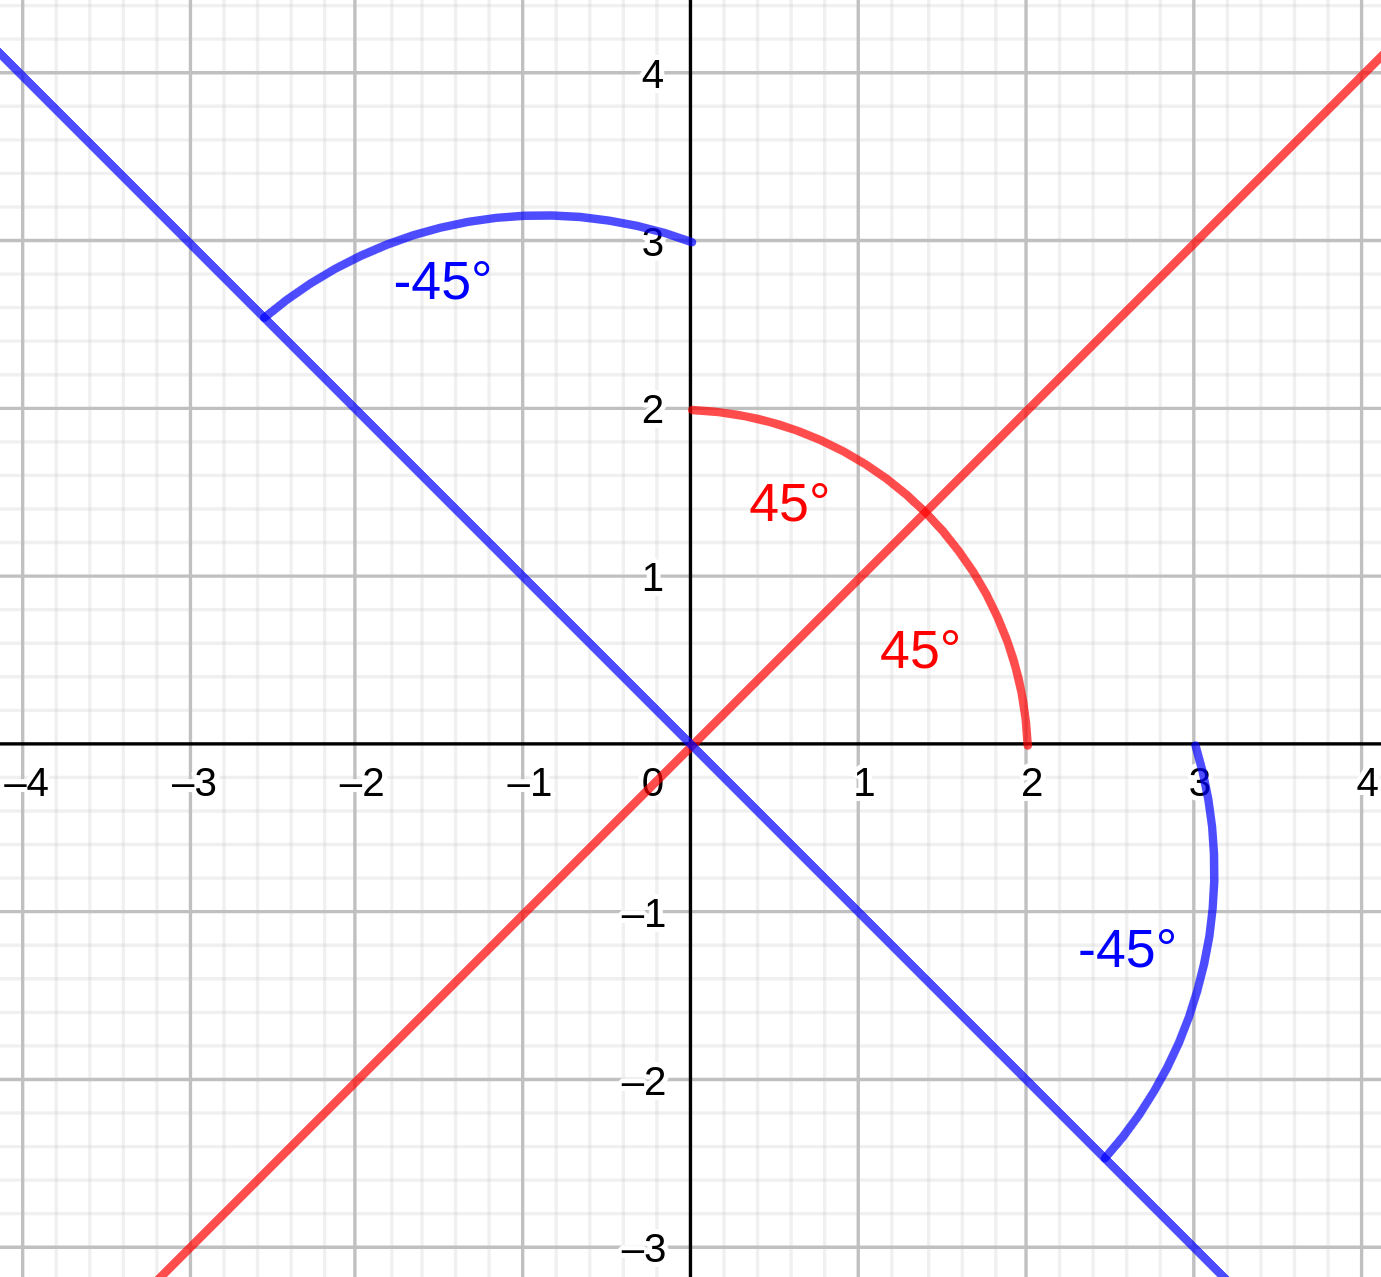
\includegraphics[scale=1]{img/ejercicios/1/2-b.png} 
\centering
\label{fig:1-2-b}
\end{figure}

Dado que cada uno de estos dos casos fija el valor del ángulo respecto al semieje positivo $z$, hay dos direcciones posible para la recta: $(1, 1, 1)$ y $(1, -1, -1)$. Eligiendo arbitrariamente la primera, con el punto dado resulta:

\begin{equation}
R: (1, 1, 1) \lambda + (1, 2, -1) 
\end{equation}

Pasando a ecuaciones implícitas:

\begin{equation}
\frac{x-1}{1} = \frac{y-2}{1} = \frac{z+1}{1} \Rightarrow \left\{ \begin{array}{ll}
x-1 = y - 2 \\
y-2 = z + 1
\end{array} \right.
\end{equation}

\begin{equation}
\tcboxmath[colback=orange!25!white,colframe=orange,title=1.2.b) Una de dos rectas]
{ R: \left\{ \begin{array}{llr}
x - &y &= 0 \\
&y - z - 3 &= 0
\end{array} \right. }
\end{equation}

\subsubsection*{1.2.c}
\label{subsubsec:1.2.c}
\addcontentsline{toc}{subsubsection}{\nameref{subsubsec:1.2.c}}

Las ecuaciones implícitas de una recta son, por definición, la intersección entre dos planos. Sólo restaría acomodar los términos y verificar si la intersección es una recta:

\begin{equation}
\left\{ \begin{array}{ll}
y-x = 0 \\
z = 4-x-y
\end{array} \right. \sim \left\{ \begin{array}{llr}
-x &+ y &= 0 \\
x &+ y + z -4 &= 0
\end{array} \right.
\end{equation}

No hace falta ninguna transformación para ver que las dos ecuaciones son l.i., y por ende determinan una única recta.

\begin{equation}
\tcboxmath[colback=orange!25!white,colframe=orange,title=1.2.c) Recta única]
{ \left\{ \begin{array}{llr}
-x &+ y &= 0 \\
x &+ y + z -4 &= 0
\end{array} \right. }
\end{equation}

\hrule
\vspace{10 pt}

\subsection*{1.3}
\label{subsec:1.3}
\addcontentsline{toc}{subsection}{\nameref{subsec:1.3}}

\textbf{En los siguientes casos, hallar $k$ de manera que exista más de un plano que pase por $v_1$, $v_2$ y $v_3$. Analizar una condición aplicable en general.} 

\begin{enumerate}[(a)]
\bfseries
\item $v_1 = (1, 0, 0)$, $v_2=(0, 1, 0)$, $v_3 = (2, -1, k)$;

\item $v_1 = (1, 1, 0)$, $v_2=(1, -1, 1)$, $v_3 = (1, -3, k)$
\end{enumerate}
\hrule

\subsubsection*{1.3.a}
\label{subsubsec:1.3.a}
\addcontentsline{toc}{subsubsection}{\nameref{subsubsec:1.3.a}}

Para que 3 puntos determinen más de un plano, deben ser colineales: sus vectores diferencia deben ser paralelos.

\begin{subequations}
\begin{align}
& \overline{v_{12}} = v_2 - v_1 = (-1, 1, 0) \\
& \overline{v_{23}} = v_3 - v_2 = (2, -2, k) \\
& \overline{v_{12}} \parallel \overline{v_{23}} \Leftrightarrow \overline{v_{12}} = \alpha \overline{v_{23}} \Leftrightarrow \left\{ \begin{array}{ll}
-1 = \alpha 2 \\
1 = \alpha (-2) \\
0 = \alpha k
\end{array} \right. \Leftrightarrow \left\{ \begin{array}{ll}
\alpha = -\frac{1}{2} \\
\alpha = -\frac{1}{2} \\
0 = \alpha k
\end{array} \right.
\end{align}
\end{subequations}

\begin{equation}
\tcboxmath[colback=orange!25!white,colframe=orange,title=1.3.a]
{ k = 0 }
\end{equation}

\subsubsection*{1.3.b}
\label{subsubsec:1.3.b}
\addcontentsline{toc}{subsubsection}{\nameref{subsubsec:1.3.b}}

Aplicando el mismo método del inciso anterior:

\begin{subequations}
\begin{align}
& \overline{v_{12}} = v_2 - v_1 = (0, -2, 1) \\
& \overline{v_{23}} = v_3 - v_2 = (0, -2, k-1) \\
& \overline{v_{12}} \parallel \overline{v_{23}} \Leftrightarrow \overline{v_{12}} = \alpha \overline{v_{23}} \Leftrightarrow \left\{ \begin{array}{ll}
0 = \alpha 0 \\
-2 = \alpha (-2) \\
1 = \alpha (k-1)
\end{array} \right. \Leftrightarrow \left\{ \begin{array}{ll}
0 = 0 \\
\alpha = 1 \\
1 = \alpha (k-1)
\end{array} \right.
\end{align}
\end{subequations}

\begin{equation}
\tcboxmath[colback=orange!25!white,colframe=orange,title=1.3.b]
{ k = 2 }
\end{equation}

Para analizar una condición general, se plantean $v_1$, $v_2$ y $v_3$ genéricos:

\begin{subequations}
\begin{align}
& v_1 = (v_{1x}, v_{1y}, v_{1z}), v_2 = (v_{2x}, v_{2y}, v_{2z}), v_3 = (v_{3x}, v_{3y}, v_{3z}) \\
& \overline{v_{12}} = v_2 - v_1 = (v_{2x} - v_{1x}, v_{2y} - v_{1y}, v_{2z} - v_{1z}) \\
& \overline{v_{23}} = v_3 - v_2 = (v_{3x} - v_{2x}, v_{3y} - v_{2y}, v_{3z} - v_{2z}) \\
& \overline{v_{12}} \parallel \overline{v_{23}} \Leftrightarrow \overline{v_{12}} = \alpha \overline{v_{23}} \Leftrightarrow \left\{ \begin{array}{ll}
v_{2x} - v_{1x} = \alpha (v_{3x} - v_{2x}) \\
v_{2y} - v_{1y} = \alpha (v_{3y} - v_{2y}) \\
v_{2z} - v_{1z} = \alpha (v_{3z} - v_{2z})
\end{array} \right.
\end{align}
\end{subequations}

Despejando $\alpha$ en las 3 ecuaciones e igualando, resulta la condición general buscada:

\begin{equation}
\tcboxmath[colback=orange!25!white,colframe=orange,title=1.3.b]
{ \frac{v_{2x} - v_{1x}}{v_{3x} - v_{2x}} = \frac{v_{2y} - v_{1y}}{v_{3y} - v_{2y}} = \frac{v_{2z} - v_{1z}}{v_{3z} - v_{2z}} }
\end{equation}

\hrule
\vspace{10 pt}

\subsection*{1.4}
\label{subsec:1.4}
\addcontentsline{toc}{subsection}{\nameref{subsec:1.4}}

\textbf{Expresar $3 \hat{i}+\hat{j}$ en la forma $u + v$, con $u$ paralelo a $\hat{i} + \hat{j}$ y $v$ perpendicular a $u$.} 

\vspace{10 pt}
\hrule
\vspace{10 pt}

Las incógnitas a determinar son $u = (u_x, u_y)$ y $v = (v_x, v_y)$. Son 4 incógnitas. La primera restricción es que su suma de $(3, 1)$:

\begin{equation}
u + v = (3, 1) \Rightarrow \left\{ \begin{array}{ll}
u_x + v_x = 3 \\
u_y + v_y = 1
\end{array} \right.
\end{equation}

La segunda restricción es $u \parallel (1, 1)$. Eso implica que $u_x = u_y$, con lo cual las incógnitas se reducen a 3.

La tercera y última restricción es $u \perp v \Rightarrow u \cdot v = 0$:

\begin{equation}
u \cdot v = 0 \Rightarrow u_x v_x + u_y v_y = 0
\end{equation}

Dado que $u_y = u_x$, esto se simplifica a:

\begin{equation}
u_x (v_x + v_y) = 0
\end{equation}

Recapitulando, las restricciones sobre las incógnitas son:

\begin{equation}
\left\{
\begin{array}{ll}
u_x + v_x = 3 \\
u_x + v_y = 1 \\
u_x (v_x + v_y) = 0
\end{array} \right.
\end{equation}

De $u_x = 0$ surgen las soluciones:

\begin{equation}
\tcboxmath[colback=orange!25!white,colframe=orange,title=1.4]
{ u = (0,0), v = (3, 1) }
\end{equation}

De $v_x + v_y = 0 \Rightarrow v_x = -v_y$, resulta:

\begin{equation}
\left\{ \begin{array}{ll}
u_x + v_x = 3 \\
u_x - v_x = 1
\end{array} \right.
\end{equation}

Sumando las ecuaciones, resulta $2 u_x = 4 \Rightarrow u_x = 2 = u_y$. Reemplazando en la primera, $2 + v_x = 3 \Rightarrow v_x = 1 \Rightarrow v_y = -1$. Así, la segunda solución posible es:

\begin{equation}
\tcboxmath[colback=orange!25!white,colframe=orange,title=1.4]
{ u = (2,2), v = (1, -1) }
\end{equation}

\hrule
\vspace{10 pt}

\subsection*{1.5}
\label{subsec:1.5}
\addcontentsline{toc}{subsection}{\nameref{subsec:1.5}}

\textbf{Calcular las siguientes distancias:} 

\begin{enumerate}[(a)]
\bfseries
\item del origen al plano de ecuación $x + 2y +3z = 4$;

\item del punto $(1, 2, 0)$ al plano de ecuación $3x - 4y - 5z = 2$;

\item del origen a la recta de ecuaciones $x + y + z = 0, 2x - y -5z = 1$.
\end{enumerate}
\hrule

\subsubsection*{1.5.a}
\label{subsubsec:1.5.a}
\addcontentsline{toc}{subsubsection}{\nameref{subsubsec:1.5.a}}

Aplicando la fórmula de la distancia entre un punto y un plano:

\begin{equation}
D = \frac{|a x_1 + b y_1 + c z_1 + d|}{\sqrt{a^2 + b^2 + c^2}} \Rightarrow D = \frac{1 \cdot 0 + 2 \cdot 0 + 3 \cdot 0 - 4}{\sqrt{1^2 + 2^2 + 3^2}} = \frac{4}{\sqrt{14}}
\end{equation}

\begin{equation}
\tcboxmath[colback=orange!25!white,colframe=orange,title=1.5.a]
{ D = \frac{4}{\sqrt{14}} \approx 1,0690 }
\end{equation}

\subsubsection*{1.5.b}
\label{subsubsec:1.5.b}
\addcontentsline{toc}{subsubsection}{\nameref{subsubsec:1.5.b}}

Aplicando la fórmula de la distancia entre un punto y un plano:

\begin{equation}
D = \frac{|a x_1 + b y_1 + c z_1 + d|}{\sqrt{a^2 + b^2 + c^2}} \Rightarrow D = \frac{3 \cdot 1 - 4 \cdot 2 - 5 \cdot 0 - 2}{\sqrt{3^2 + (-4)^2 + (-5)^2}} = \frac{7}{\sqrt{50}}
\end{equation}

\begin{equation}
\tcboxmath[colback=orange!25!white,colframe=orange,title=1.5.b]
{ D = \frac{7}{\sqrt{50}} \approx 0,98995 }
\end{equation}

\subsubsection*{1.5.c}
\label{subsubsec:1.5.c}
\addcontentsline{toc}{subsubsection}{\nameref{subsubsec:1.5.c}}

Pasando la recta a forma paramétrica:

\begin{subequations}
\begin{align}
& \left\{ \begin{array}{lr}
x + y + z &= 0 \\
2x - y - 5z &= 1
\end{array} \right. \overset{F_2 \leftarrow -2F_1 + F_2}{\sim} \left\{ \begin{array}{ll}
x + y + z = 0 \\
-3y -7z = 1
\end{array} \right. \\
& \text{Despejando z de } F_2: -7z = 1 + 3y \Rightarrow z = -\frac{1}{7} -\frac{3}{7} y \\
& \text{Reemplazando en } F_1: x + y - \frac{1}{7} -\frac{3}{7} y = 0 \Rightarrow x + \frac{4}{7} y = \frac{1}{7} \Rightarrow x = \frac{1}{7} -\frac{4}{7} y \\
& R: \left( \frac{1}{7} -\frac{4}{7}y, y, -\frac{1}{7} -\frac{3}{7} y \right) = \left( \frac{1}{7}, 0, -\frac{1}{7} \right) + \left( -\frac{4}{7}, 1, -\frac{3}{7} \right) y \\
& R: (-4, 7, -3) t + (1, 0, -1)
\end{align}
\end{subequations}

Se busca el valor $t_0$ tal que el vector $P_0 - R(t_0)$ sea ortogonal al vector dirección de la recta. En este caso, $P_0 = (0, 0, 0)$:

\begin{subequations}
\begin{align}
& \{(0, 0, 0) - [(-4, 7, -3) t_0 + (1, 0, -1)]\} \cdot (-4, 7, -3) = 0 \\
& (4 t_0 - 1, -7 t_0, 3 t_0 + 1) \cdot (-4, 7, -3) = 0 \\
& -16 t_0 + 4 -49 t_0 -9 t_0 -3 = 0 \Leftrightarrow -74 t_0 + 1 = 0 \Leftrightarrow t_0 = \frac{1}{74} 
\end{align}
\end{subequations}

Conocido $t_0$, se puede calcular $R(t_0)$, y finalmente $d = ||P_0 - R(t_0)||$:

\begin{subequations}
\begin{align}
& R(t_0) = (-4, 7, -3) \frac{1}{74} + (1, 0, -1) = \left( \frac{70}{74}, \frac{7}{74}, -\frac{77}{74} \right) \\
& d = ||(0,0,0) - R(t_0)|| = ||R(t_0)|| = \frac{\sqrt(70^2 + 7^2 + 77^2)}{74}
\end{align}
\end{subequations}

\begin{equation}
\tcboxmath[colback=orange!25!white,colframe=orange,title=1.5.c]
{ d = \frac{\sqrt{10878}}{74} \approx 1,4094 }
\end{equation}

\hrule
\vspace{10 pt}

\subsection*{1.6}
\label{subsec:1.6}
\addcontentsline{toc}{subsection}{\nameref{subsec:1.6}}

\textbf{Hallar la distancia de la recta de ecuaciones $x - 2 = (y + 3)/2 = (z-1)/4$ al plano de ecuación $2y -z = 1$.} 
\vspace{10 pt}
\hrule
\vspace{10 pt}

Si un plano y una recta se cortan, la distancia entre ambos es nula. Por ende, sólo puede haber distancia no nula entre ambos cuando son paralelos. En dicho caso, la distancia entre cualquier punto de la recta y el plano será la misma, y puede calcularse con la fórmula ya conocida para la distancia entre un plano y un punto.

Por lo tanto, el primer paso es determinar la intersección entre la recta y el plano:

\begin{subequations}
\begin{align}
& \left\{ \begin{array}{ll}
x-2 = \frac{y+3}{2} \\
\frac{y+3}{2} = \frac{z - 1}{4} \\
2y -z = 1
\end{array} \right. \sim \left\{ \begin{array}{lllr}
x&-\frac{1}{2}y & &- \frac{7}{2} = 0 \\
&\frac{1}{2}y &-\frac{1}{4}z &+ \frac{7}{4} = 0 \label{eq:1.6} \\
&2y &- z &- 1 = 0
\end{array} \right. \overset{F_3 \leftarrow -4 F_2 + F_3}{\sim} \\
& \left\{ \begin{array}{lllr}
x -&\frac{1}{2} y &&-\frac{7}{2} = 0 \\
&\frac{1}{2} y &-\frac{1}{4}z + &\frac{7}{4} = 0 \\
&&&-8 = 0
\end{array} \right.
\end{align}
\end{subequations}

Se llegó a un absurdo, por lo tanto no existe intersección, y el plano y la recta son paralelos. Para calcular la distancia, se toma un punto arbitrario de la recta y se calcula su distancia al plano. Observando las dos primeras ecuaciones en el sistema de la ecuación \ref{eq:1.6}, que corresponden a la recta, se observa que $y$ puede funcionar como parámetro. Ergo, definiendo arbitrariamente $y = 0$, resultan $x=\frac{7}{2}$ y $z=7$. Por lo tanto, el punto $(\frac{7}{2}, 0, 7)$ pertenece a la recta.

Por otro lado, inspeccionando la ecuación del plano, resultan $(a, b, c) = (0, 2, -1)$ y $d = -1$. Evaluando la fórmula:

\begin{equation}
d(\Pi, P_1) = \frac{|a x_1 + b y_1 + c z_1 + d|}{\sqrt{a^2 + b^2 + c^2}} = \frac{|0 \cdot \frac{7}{2} + 2 \cdot 0 -1 \cdot 7 - 1 |}{\sqrt{0^2 + 2^2 + 1^2}} = \frac{8}{\sqrt{5}}
\end{equation}

\begin{equation}
\tcboxmath[colback=orange!25!white,colframe=orange,title=1.6]
{ d = \frac{8}{\sqrt{5}} \approx 3,5777 }
\end{equation}

\hrule
\vspace{10 pt}

\subsection*{1.7}
\label{subsec:1.7}
\addcontentsline{toc}{subsection}{\nameref{subsec:1.7}}

\textbf{Dados los vectores $u = 2 \hat{i} + \hat{j} -2\hat{k}$ y $v = 2\hat{i} - 2\hat{j}-\hat{k}$} hallar 

\begin{enumerate}[(a)]
\bfseries
\item el ángulo entre $u$ y $v$;

\item $|u|$

\item $3u - 2v$

\item un vector unitario paralelo a $u$.
\end{enumerate}
\hrule

\subsubsection*{1.7.a}
\label{subsubsec:1.7.a}
\addcontentsline{toc}{subsubsection}{\nameref{subsubsec:1.7.a}}

Para dos vectores no nulos $x$ e $y$, el producto escalar canónico garantiza que:

\begin{equation}
\cos \theta(x,y) = \frac{x \cdot y}{||x|| ||y||}
\label{eq:angvec}
\end{equation}

En la igualdad de la ecuación \ref{eq:angvec}, $\theta(x, y)$ es el ángulo entre los dos vectores, medido desde $x$. Aplicando a este caso,

\begin{equation}
\cos \theta(u,v) = \frac{(2, 1, -2) \cdot (2, -2, -1)}{\sqrt{2^2 + 1^2 + 2^2} \sqrt{2^2 + 2^2 + 1}} \Rightarrow \theta(u, v) =  \arccos \frac{2 \cdot 2 + 1 \cdot (-2) -2 (-1)}{\sqrt{9} \sqrt{9}}
\end{equation}

\begin{equation}
\tcboxmath[colback=orange!25!white,colframe=orange,title=1.7.a]
{ \theta(u, v) = \arccos \frac{4}{9} \approx 1,11 \mathop{rad} \approx 63,612^{\circ} }
\end{equation}

\subsubsection*{1.7.b}
\label{subsubsec:1.7.b}
\addcontentsline{toc}{subsubsection}{\nameref{subsubsec:1.7.b}}

$||u|| = \sqrt{2^2 + 1^2 + 2^2} = 3$

\begin{equation}
\tcboxmath[colback=orange!25!white,colframe=orange,title=1.7.b]
{ ||u|| = 3 }
\end{equation}

\subsubsection*{1.7.c}
\label{subsubsec:1.7.c}
\addcontentsline{toc}{subsubsection}{\nameref{subsubsec:1.7.c}}

$3u - 2v = (6, 3, -6) - (4, -4, -2) = (2, 7, -4)$

\begin{equation}
\tcboxmath[colback=orange!25!white,colframe=orange,title=1.7.c]
{ 3u - 2v = (2, 7, -4) }
\end{equation}

\subsubsection*{1.7.d}
\label{subsubsec:1.7.d}
\addcontentsline{toc}{subsubsection}{\nameref{subsubsec:1.7.d}}

Multiplicar un vector por el recíproco de su propia norma lo hace unitario.

$\hat{u} = \frac{u}{||u||} = \frac{1}{3} (2, 1, -2)$
 
\begin{equation}
\tcboxmath[colback=orange!25!white,colframe=orange,title=1.7.d]
{ \hat{u} = \left( \frac{2}{3}, \frac{1}{3}, -\frac{2}{3} \right) }
\end{equation}

\hrule
\vspace{10 pt}

\subsection*{1.8}
\label{subsec:1.8}
\addcontentsline{toc}{subsection}{\nameref{subsec:1.8}}

\textbf{Responder a cada uno de los siguientes problemas}

\begin{enumerate}[(a)]
\bfseries
\item Probar que el triángulo de vértices $(1, -1, 2)$, $(3, 3, 8)$ y $(2, 0, 1)$ es rectángulo.

\item ¿Cuánto miden los ángulos del triángulo de vértices $(1, 0, 0)$, $(0, 2, 0)$ y $(0, 0, 3)$?

\item ¿Cuánto mide el volumen del tetraedro de vértices $(1, 0, 0)$, $(1, 2, 0)$, $(2, 2, 2)$ y $(0, 3, 2)$?

\item ¿Cuánto mide el ángulo entre la diagonal de un cubo y una de sus aristas?

\item ¿Cuánto vale el área del triángulo de vértices $(1, 1, 0)$, $(3, 0, 2)$ y $(2, -1, 1)$? ¿Es equilátero?

\item Hallar los valores de $k$ para los que los puntos $(1, 1, -1)$, $(0, 3, -2)$, $(-2, 1, 0)$ y $(k, 0, 2)$ son coplanares; determinar en esos casos una ecuación del plano que los contiene.

\item Hallar el área del paralelogramo dos de cuyos lados son los segmentos que unen el origen con $(1, 0, 1)$ y $(0, 2, 1)$.
\end{enumerate}
\hrule

\subsubsection*{1.8.a}
\label{subsubsec:1.8.a}
\addcontentsline{toc}{subsubsection}{\nameref{subsubsec:1.8.a}}

Los tres puntos definen un triángulo: sus lados están dados por los vectores resta. Obśervese la figura \ref{fig:1-8-a}.

\begin{figure}[ht]
\caption{Triángulo definido por puntos}
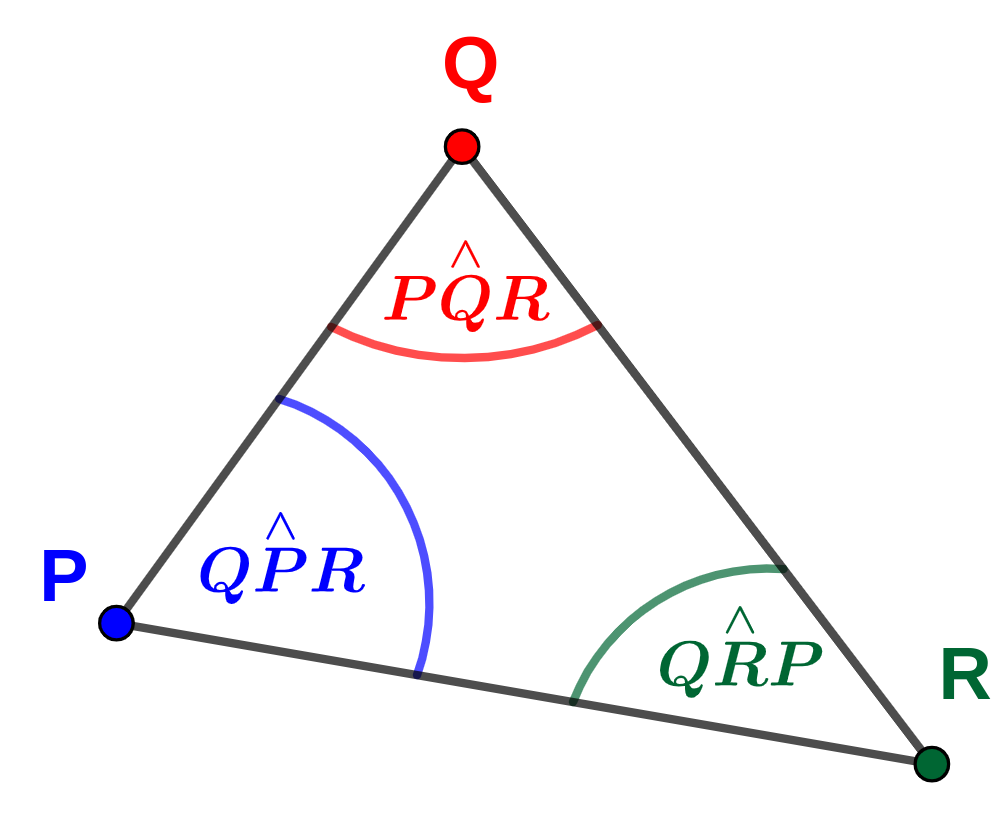
\includegraphics[scale=1]{img/ejercicios/1/8-a.png} 
\centering
\label{fig:1-8-a}
\end{figure}

Los ángulos internos están dados por el ángulo entre los vectores resta; el sentido de la recta es importante. Concretamente:

\begin{subequations}
\begin{align}
& P = (1, -1, 2) \\
& Q = (3, 3, 8) \\
& R = (2, 0, 1) \\
& Q\overset{\wedge}{P}R = \theta(\overline{PR}, \overline{PQ}) = \theta(R-P, Q-P) = arccos \left(\frac{(1,1,-1) \cdot (2, 4, 6)}{||(1, 1, -1)|| ||(2,4,6)||} \right) = 90^{\circ} \\
& P\overset{\wedge}{Q}R = \theta(\overline{QP}, \overline{QR}) = \theta(P-Q, R-Q) = \theta((-2,-4,-6),(-1, -3, -7)) \approx 13,032^{\circ} \\
& R\overset{\wedge}{R}P = \theta(\overline{RQ}, \overline{RP}) = \theta(Q-R, P-R) = \theta((1,3,7),(-1, -1, 1)) \approx 76.968^{\circ}
\end{align}
\end{subequations}

\begin{equation}
\tcboxmath[colback=orange!25!white,colframe=orange, title=1.8.a]
{ \overset{\wedge}{P} = 90^{\circ}, \overset{\wedge}{Q} \approx 13,032^{\circ}, \overset{\wedge}{R} \approx 76,968^{\circ} }
\end{equation}

Con demostrar que uno de los ángulos es de 90 grados, era suficiente. Sólo se calcularon los otros dos para verificar que sumen 180 grados (recordar que la suma de los ángulos internos de un triángulos siempre da 180 grados).

\subsubsection*{1.8.b}
\label{subsubsec:1.8.b}
\addcontentsline{toc}{subsubsection}{\nameref{subsubsec:1.8.b}}

Mismo procedimiento que inciso anterior, distintos puntos.

\begin{subequations}
\begin{align}
& P = (1, 0, 0) \\
& Q = (0, 2, 0) \\
& R = (0, 0, 3) \\
& \overset{\wedge}{P} = \theta(R-P, Q-P) = arccos \left(\frac{(-1,0,3) \cdot (-1, 2, 0)}{||(-1, 0, 3)|| ||(-1,2,0)||} \right) \\
& \overset{\wedge}{Q} = \theta(P-Q, R-Q) = \theta((1,-2,0),(0, -2, 3)) \\
& \overset{\wedge}{R} = \theta(Q-R, P-R) = \theta((0,2,-3),(1, 0, -3))
\end{align}
\end{subequations}

\begin{equation}
\tcboxmath[colback=orange!25!white,colframe=orange, title=1.8.b]
{ \overset{\wedge}{P} \approx 81,870, \overset{\wedge}{Q} \approx 60,255, \overset{\wedge}{R} \approx 37,875 }
\end{equation}

\subsubsection*{1.8.c}
\label{subsubsec:1.8.c}
\addcontentsline{toc}{subsubsection}{\nameref{subsubsec:1.8.c}}

El volumen de un tetraedro irregular puede calcularse con la siguiente fórmula:

\begin{equation}
V = \frac{1}{3} A_b h \label{eq:voltetr}
\end{equation}

Donde $A_b$ es el área de una de las caras triangulares, y $h$ es la distancia entre dicha cara y el punto que no pertenece a ella. Esto sugiere que una forma práctica de calcular el volumen es hallar el área de una cara cualquiera, y calcular $h$ como la distancia entre el plano de los 3 puntos de esa cara y el punto restante.

Se definen los cuatro puntos del tetraedro como:

\begin{align}
P = (1, 0, 0) \\
Q = (1, 2, 0) \\
R = (2, 2, 2) \\
S = (0, 3, 2)
\end{align}

Graficando estos puntos en $\Bbb R^3$, se obtiene la figura \ref{fig:1-8-c}.

\begin{figure}[ht]
\caption{Tetraedro}
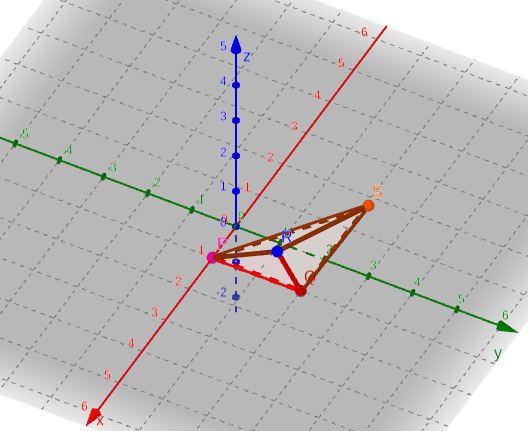
\includegraphics[scale=0.6]{img/ejercicios/1/8-c.png} 
\centering
\label{fig:1-8-c}
\end{figure}

Obsérvese que tomando tres puntos cualquiera, se tiene una de las caras triangulares del tetraedro. Por la simetría del tetraedro, cualquiera de dichas caras puede interpretarse como la base en la fórmula. La altura estará dada por la distancia perpendicular entre el plano determinado por los 3 puntos de la base elegida, y el punto restante. Concretamente, la cara $PQR$ es un triángulo rectángulo, por lo tanto, su área puede obtenerse directamente:

\begin{equation}
A_b = \frac{1}{2} b h = \frac{1}{2} ||\overline{PQ}|| ||\overline{QR}|| = \frac{1}{2} ||Q-P|| ||R-Q|| \approx 2,2361
\end{equation}

La normal $(a,b,c)$ del plano determinado por $P$, $Q$ y $R$ está dada por el producto vectorial de los vectores resta:

\begin{equation}
(a,b,c) = \overline{PQ} \times \overline{PR} = (Q-P) \times (R-P) = (4, 0, -2)
\end{equation}

Y el parámetro $d$ en la ecuación del plano $a x + b y + c z + d = 0$ se obtiene evaluando en cualquier punto del plano:

\begin{equation}
d = -(a x_0 + b y_0 + c z_0) \overset{(x_0, y_0, z_0) = P}{\Rightarrow} = -4
\end{equation}

La altura del tetraedro con esta base será entonces la distancia entre el plano $PQR$ y el punto $S$:

\begin{subequations}
\begin{align}
h = \frac{|a x_1 + b y_1 + c z_1 + d|}{\sqrt(a^2 + b^2 + c^2)} \overset{(x_1, y_1, z_1) = S}{\Longrightarrow} h = \frac{|4 \cdot 0 + 0 \cdot 3 -2 \cdot 2 -4|}{\sqrt{4^2 + 0^2 + 2^2}} \\
h = \frac{8}{\sqrt{20}} \approx 1,7889
\end{align}
\end{subequations}

Finalmente, con $A_b$ y $h$ resulta:

\begin{equation}
\tcboxmath[colback=orange!25!white,colframe=orange, title=1.8.c) Volumen del tetraedro]
{ V = \frac{1}{3} A_b h \approx 1.3333 }
\end{equation}

A modo de verificación, existe una fórmula más directa en base a los vértices:

\begin{equation}
V = \frac{1}{6} ((\overline{PQ} \times \overline{PR}) \cdot \overline{PS}) \approx 1.3333
\end{equation}

\subsubsection*{1.8.d}
\label{subsubsec:1.8.d}
\addcontentsline{toc}{subsubsection}{\nameref{subsubsec:1.8.d}}

Colocando un cubo de lado $a$ con una esquina inferior en el origen, y dos caras en el sentido de los semiejes positivos, una de las dos diagonales del cubo es el vector que va del origen a la esquina superior opuesta en el punto $(a,a,a)$. Dicho vector es $(a, a, a) - (0, 0, 0) = (a, a, a)$. Tomando una arista de las tres adyacentes al origen, como por ejemplo $(a, 0, 0)$, resulta:

\begin{equation}
\theta = \arccos \frac{(a,a,a) \cdot (a, 0, 0)}{||(a,a,a)|| ||(a,0,0)||} = \arccos \frac{a^2}{\sqrt{3a^2} \sqrt{a^2}} = \arccos \frac{1}{\sqrt{3}}
\end{equation}

\begin{equation}
\tcboxmath[colback=orange!25!white,colframe=orange, title=1.8.d) Ángulo entre arista de cubo y diagonal]
{ \theta = \arccos \frac{\sqrt{3}}{3} A_b h \approx 54,736^{\circ} }
\end{equation}

Por la simetría del cubo, cualquiera de las otras dos aristas dará el mismo valor.

\subsubsection*{1.8.e}
\label{subsubsec:1.8.e}
\addcontentsline{toc}{subsubsection}{\nameref{subsubsec:1.8.e}}

Sean los puntos del triángulo:

\begin{subequations}
\begin{align}
P = (1, 1, 0) \\
Q = (3, 0, 2) \\
R = (2, -1, 1)
\end{align}
\end{subequations}

Las longitudes de los lados son simplemente las normas de los vectores que unen los vértices. Tomando como referencia la figura \ref{fig:1-8-e}, resulta:

\begin{figure}[ht]
\caption{Triángulo}
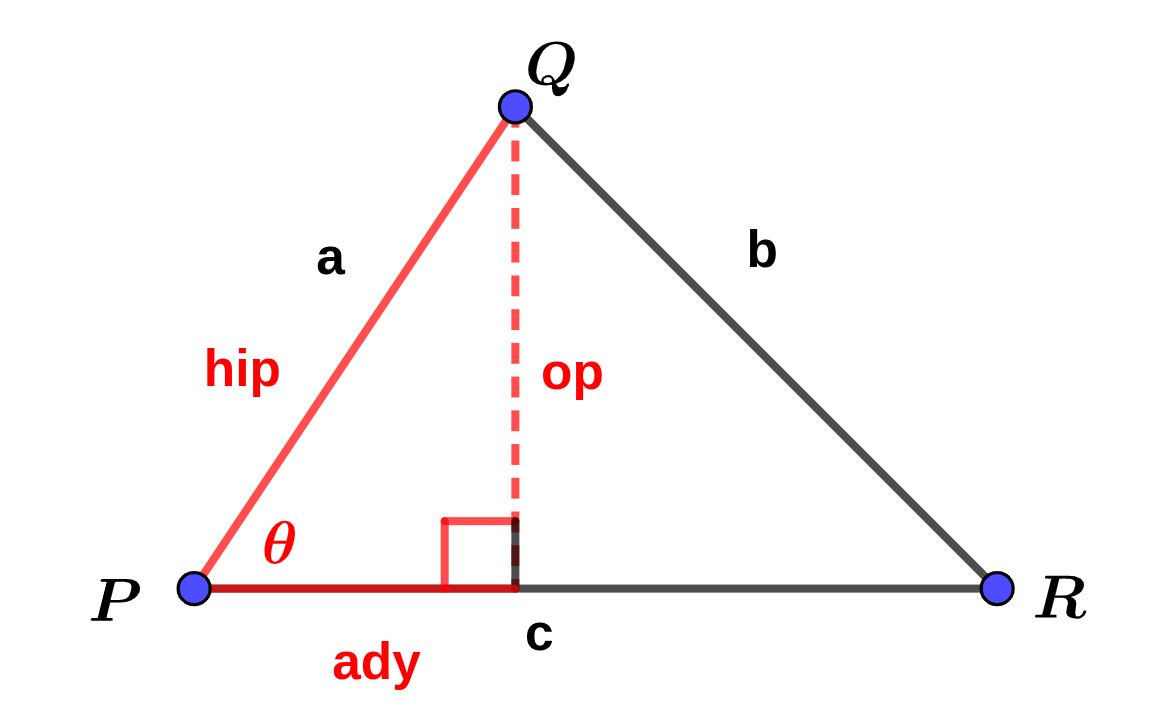
\includegraphics[scale=0.8]{img/ejercicios/1/8-e.png} 
\centering
\label{fig:1-8-e}
\end{figure}

\begin{subequations}
\begin{align}
a = ||\overline{PQ}|| = ||Q-P|| = 3 \\
b = ||\overline{QR}|| = ||R-Q|| \approx 1,7321 \\
c = ||\overline{PR}|| = ||R-P|| \approx 2,4495
\end{align}
\end{subequations}

Claramente el triángulo no es equilátero. Aplicando trigonometría y ángulo entre vectores con las referencias de la figura \ref{fig:1-8-e}, resulta:

\begin{subequations}
\begin{align}
& A = \frac{1}{2} \underbrace{||R-P||}_{\text{base}} \underbrace{ \mathop{op} }_{\text{altura}} \\
& \sin \theta = \frac{\mathop{op}}{||Q-P||} \\
& \mathop{op} = \sin (\theta) ||Q-P|| = \sin( \arccos \left( \frac{\overline{PQ} \cdot \overline{PR} }{||\overline{PQ}|| ||\overline{PR}||} \right) ) ||Q-P||
\end{align}
\end{subequations}

\begin{equation}
\tcboxmath[colback=orange!25!white,colframe=orange,title=1.8.e]
{ A \approx 2,1213 }
\end{equation}

Verificando con la fórmula de Herón:

\begin{subequations}
\begin{align}
& A = \frac{1}{2} \sqrt{s (s-a) (s-b) (s-c)} \\
& s \approx 3,5908 \\
& A \approx 2,1213
\end{align}
\end{subequations}

\subsubsection*{1.8.f}
\label{subsubsec:1.8.f}
\addcontentsline{toc}{subsubsection}{\nameref{subsubsec:1.8.f}}

Hay tres puntos fijos y uno variable. El plano determinado por los 3 puntos fijos será:

\begin{subequations}
\begin{align}
& P = (1, 1, -1) \\
& Q = (0, 3, -2) \\
& R = (-2, 1, 0) \\
& \overline{PQ} = Q-P = (-1 2 1) \\
& \overline{PR} = R-P = (-3 0 1) \\
& (a,b,c) = \overline{PQ} \times \overline{PR} = (2, 4, 6) \\
& d = -(a x_0 + b y_0 + c z_0) = -(2 \cdot -2 + 4 \cdot 1 + 6 \cdot 0) = 0
\end{align}
\end{subequations}

La ecuación del plano resulta entonces $2x + 4y + 6z = 0$. Para que el punto $(k, 0, 2)$ pertenezca al plano, debe satisfacer su ecuación:

\begin{equation}
2k + 4 \cdot 0 + 6 \cdot 2 = 0 \Rightarrow 2k = -12
\end{equation}

Finalmente:

\begin{equation}
\tcboxmath[colback=orange!25!white,colframe=orange,title=1.8.f]
{ k = -6 }
\end{equation}

\begin{equation}
\tcboxmath[colback=orange!25!white,colframe=orange,title=1.8.f]
{ \Pi: \{ 2x + 4y + 6z = 0 }
\end{equation}

\subsubsection*{1.8.g}
\label{subsubsec:1.8.g}
\addcontentsline{toc}{subsubsection}{\nameref{subsubsec:1.8.g}}

El área de un paralelogramo está relacionada con la norma del producto vectorial entre dos lados no paralelos:

\begin{equation}
A = ||x \times y|| = ||x|| ||y|| \sin(\theta(x,y))
\end{equation}

Para este caso:

\begin{equation}
\tcboxmath[colback=orange!25!white,colframe=orange,title=1.8.g]
{ A = ||(1, 0, 1) \times (0, 2, 1)|| = 3 }
\end{equation}

Verificación geométrica: el área del paralelogramo es $b h$, donde $b$ es la longitud de una base, y $h$ es la altura perpendicular hacia la base paralela. Tomando el vector $(0, 2, 1)$ como la base, y las referencias de la figura \ref{fig:1-8-g}, la altura $h$ del paralelogramo puede obtenerse de la siguiente manera:

\begin{figure}[ht]
\caption{Área paralelogramo}
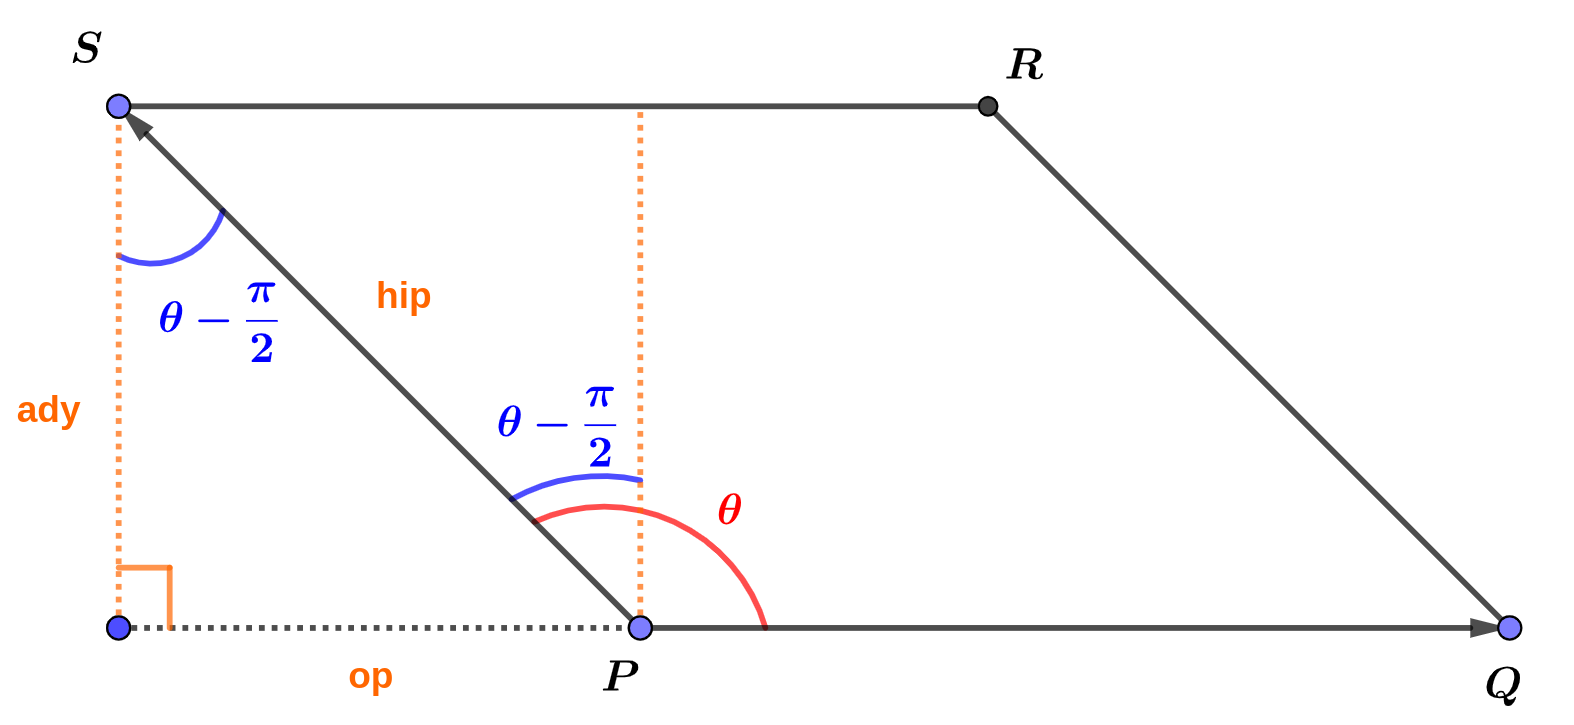
\includegraphics[scale=1]{img/ejercicios/1/8-g.png} 
\centering
\label{fig:1-8-g}
\end{figure}

\begin{equation}
\cos \left( \theta - \frac{\pi}{2} \right) = \frac{h}{||S-P||}
\end{equation}

Recordando la identidad $\cos(\alpha - \frac{\pi}{2}) = \sin(\alpha)$:

\begin{subequations}
\begin{align}
& \sin(\theta) = \frac{h}{||S-P||} \\
& \theta = \arccos \left( \frac{(Q-P) \cdot (S-P)}{||Q-P|| ||S-P||} \right) \\
& P = (0,0,0), Q = (0,2,1), S = (1, 0, 1) \\
& \theta \approx 71,565^{\circ} \\
& h = \sin(\theta) * ||S|| \approx 1,3416 \\
& A = ||Q-P|| h = 3
\end{align}
\end{subequations}

\hrule
\vspace{10 pt}

\subsection*{1.9}
\label{subsec:1.9}
\addcontentsline{toc}{subsection}{\nameref{subsec:1.9}}

\textbf{Dados $v_1 = (3, 1, 1)$, $v_2 = (2, 1, -1)$ y $v_3 = (1, 1, -1)$}

\begin{enumerate}[(a)]
\bfseries
\item Hallar la componente de $v_3$ en el plano generado por $v_1$ y $v_2$

\item Hallar la componente de $v_3$ normal a $v_1$ y $v_2$

\item ¿Es cierto que la suma de los cuadrados de las normas de los vectores de los dos incisos anteriores debe ser el cuadrado de la norma de $v_3$? Justificar

\item Hallar un vector $v$ en el plano generado por $v_1$ y $v_2$ perpendicular a $v_1$ y tal que al área del rectángulo que tiene $v$ y $v_1$ como lados es igual a la del paralelogramo que tiene $v_2$ y $v_1$ como lados. Hacer un dibujo ilustrativo.

\item Hallar, si lo hay, un vector en la recta que une los extremos de $v_1$ y $v_3$, perpendicular a $v_2$. 
\end{enumerate}
\hrule

\subsubsection*{1.9.a}
\label{subsubsec:1.9.a}
\addcontentsline{toc}{subsubsection}{\nameref{subsubsec:1.9.a}}

Dados dos vectores, la normal $\overline{N} = (a, b, c)$ al plano que generan está dada por su producto vectorial:

\begin{equation}
\overline{N} = (a, b, c) = v_1 \times v_2 = (3, 1, 1) \times (2, 1, -1) = (-2, 5, 1)
\end{equation}

Como los vectores $v_1$ y $v_2$ parten del origen, dicho punto está incluido en el plano, y por ende $d = 0$ en la ecuación del plano:

\begin{equation}
\Pi: -2x + 5y + z = 0
\end{equation}

Cuando se habla de componentes normal y paralela de un vector respecto a un plano, ello consiste en descomponer ese vector en la suma de dos vectores, uno paralelo a $\overline{N}$, y otro ortogonal:

\begin{subequations}
\begin{align}
& v_3 = v_{3\perp} + v_{3\parallel} \\
& v_{3\perp}: \text{Componente de } v_3 \text{ en el plano} \\
& v_{3\parallel}: \text{Componente de } v_3 \text{ normal al plano} \\
\end{align}
\end{subequations}

Multiplicando (con producto escalar) la descomposición de $v3$ por $\overline{N}$ miembro a miembro:

\begin{equation}
v_3 \cdot \overline{N} = \underbrace{ v_{3\perp} \cdot \overline{N} }_{0} + v_{3\parallel} \cdot \overline{N}
\end{equation}

Dado que $v_{3\parallel}$ es paralelo a $\overline{N}$, $v_{3\parallel} = \lambda \overline{N}$:

\begin{subequations}
\begin{align}
& v_3 \cdot \overline{N} = \lambda \overline{N} \cdot \overline{N} \\
& 2 = \lambda 30 \Rightarrow \lambda = \frac{1}{15} \Rightarrow v_{3\parallel} = \frac{1}{15} (-2, 5, 1)
\end{align}
\end{subequations}

Conocido $v_{3\parallel}$, $v_{3\perp}$ sale con una simple resta:

\begin{equation}
v_3 = v_{3\perp} + v_{3\parallel} \Rightarrow v_{3\perp} = v_3 - v_{3\parallel} \Rightarrow v_{3\perp} = \frac{1}{15} (17, 10, -16)
\end{equation}

La componente en el plano es entonces:

\begin{equation}
\tcboxmath[colback=orange!25!white,colframe=orange,title=1.9.a]
{ v_{3\perp} = \frac{1}{15} (17, 10, -16) }
\end{equation}

\subsubsection*{1.9.b}
\label{subsubsec:1.9.b}
\addcontentsline{toc}{subsubsection}{\nameref{subsubsec:1.9.b}}

Del inciso anterior, se obtuvo la componente normal:

\begin{equation}
\tcboxmath[colback=orange!25!white,colframe=orange,title=1.9.b]
{ v_{3\perp} = \frac{1}{15} (-2, 5, 1) }
\end{equation}

\subsubsection*{1.9.c}
\label{subsubsec:1.9.c}
\addcontentsline{toc}{subsubsection}{\nameref{subsubsec:1.9.c}}

Es verdadero. Para este caso particular, puede verificarse numéricamente:

\begin{subequations}
\begin{align}
& ||v_{3\perp}||^2 + ||v_{3\parallel}||^2 = 3 \\
& ||v_3||^2 = 3
\end{align}
\end{subequations}

De manera más general, alcanza con ver que cuando el ángulo entre los vectores sumandos es de 90 grados, siempre forman un triángulo rectángulo con el vector suma y por ende se verifica el teorema de Pitágoras. Esto puede observarse en la figura \ref{fig:1-9-c}.

\begin{figure}[ht]
\caption{Suma de dos vectores ortogonales}
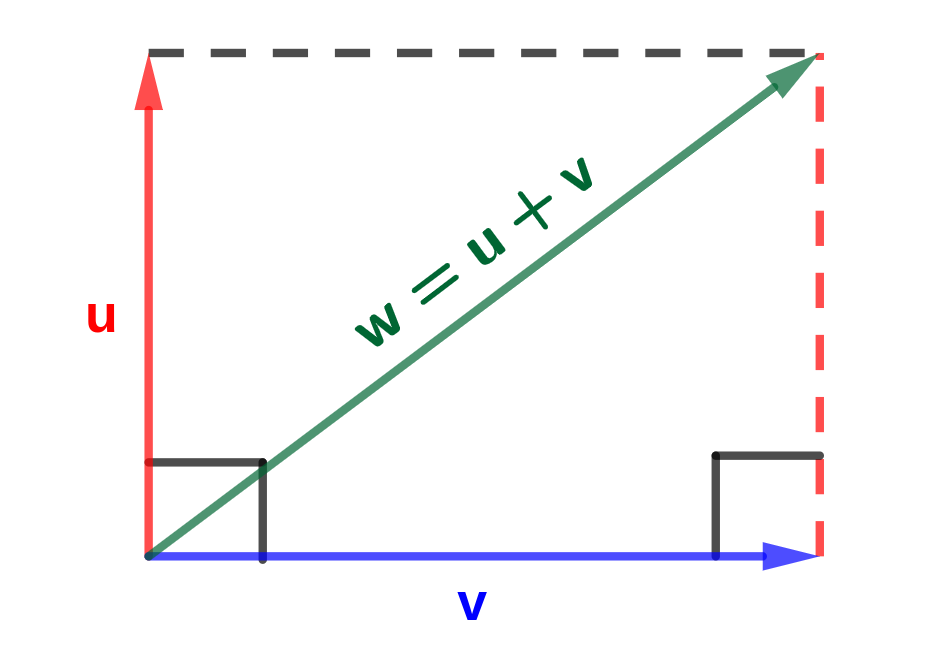
\includegraphics[scale=1]{img/ejercicios/1/9-c.png} 
\centering
\label{fig:1-9-c}
\end{figure}

\subsubsection*{1.9.d}
\label{subsubsec:1.9.d}
\addcontentsline{toc}{subsubsection}{\nameref{subsubsec:1.9.d}}

Un dibujo ilustrativo posible sería el de la figura \ref{fig:1-9-d}. Los vectores $v_1$ y $v_2$ (azul) son los que determinan el plano cuya normal es el vector $N$ (rojo). De los infinitos vectores $v$ (verde) perpendiculares a $v_1$, se busca aquellos con una norma específica, por lo que es esperable que la solución sea una circunferencia en el espacio tridimensional. 

\begin{figure}[ht]
\caption{Rectángulo y paralelogramo en $\Bbb R^3$}
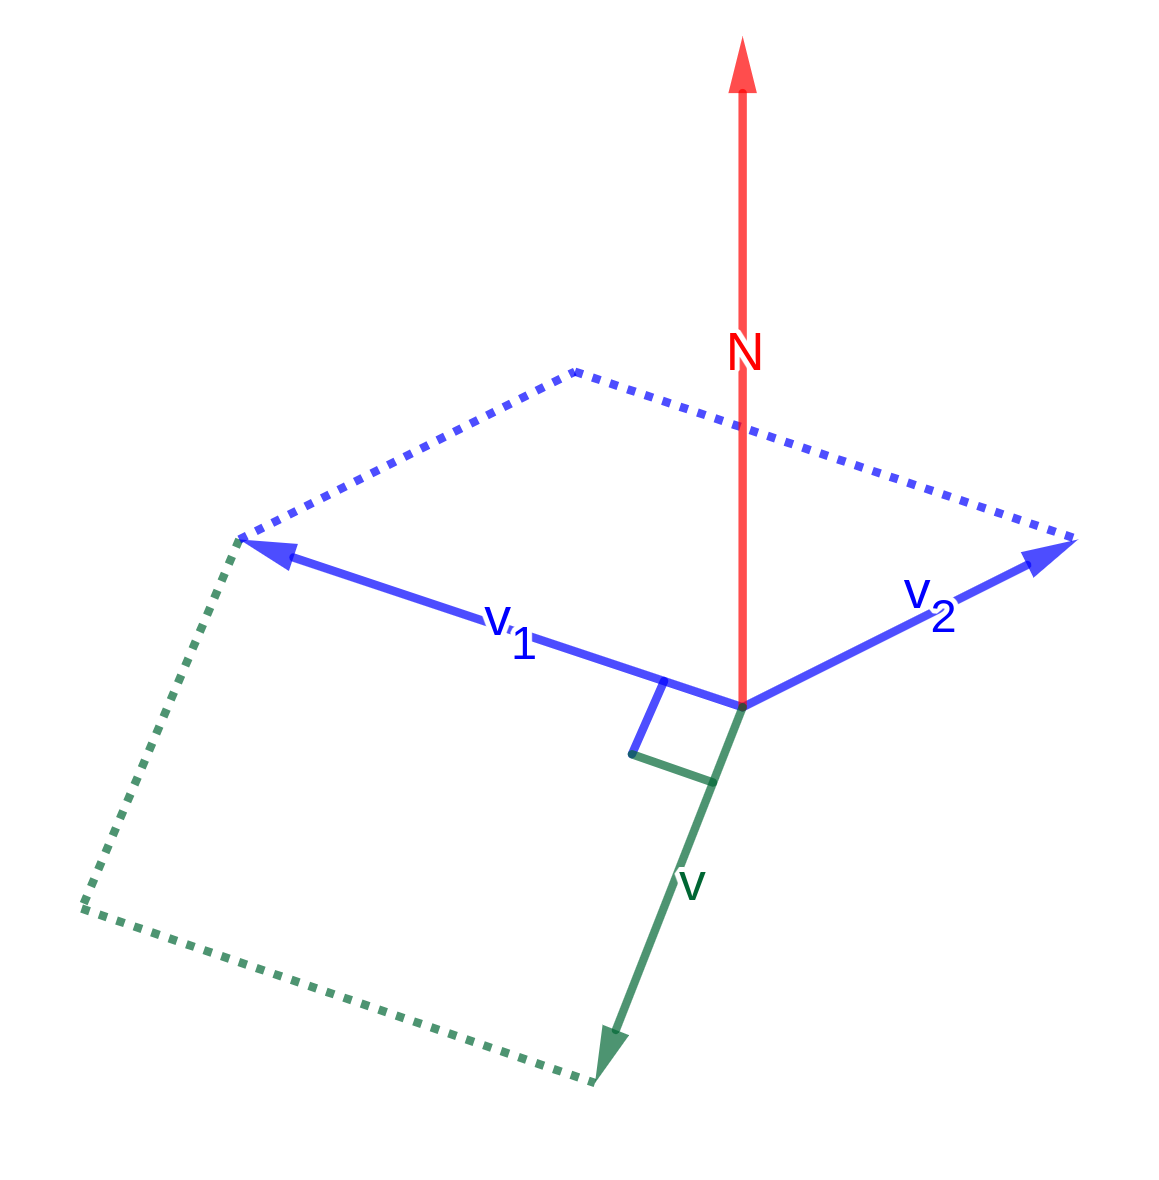
\includegraphics[scale=1]{img/ejercicios/1/9-d.png} 
\centering
\label{fig:1-9-d}
\end{figure}

Sea entonces $v = (v_x, v_y, v_z)$. Exigiendo que este vector sea perpendicular a $v_1$ resulta:

\begin{equation}
v \cdot v_1 = 0 \Rightarrow (v_x, v_y, v_z) \cdot (3, 1, 1) = 0 \Rightarrow 3 v_x + v_y + v_z = 0
\end{equation}

Por otro lado, la restricción de igualdad de áreas establece que:

\begin{equation}
||v|| ||v_1|| = ||v_1 \times v_2|| \Rightarrow ||v|| = \frac{||v_1 \times v_2||}{||v_1||} = k \approx 2,7273
\end{equation}

Como se previó, la solución es una circunferencia en un plano:

\begin{equation}
\left\{
\begin{array}{ll}
3 v_x + v_y + v_z = 0 \\
v_x^2 + v_y^2 + v_z^2 = k^2 \approx 7,4382
\end{array}
\right.
\end{equation}

De estos infinitos vectores posibles, se puede elegir uno haciendo arbitrariamente $v_z = 0$. Eso determinará las otras dos componentes:

\begin{equation}
\left\{
\begin{array}{ll}
3 v_x + v_y = 0 \\
v_x^2 + v_y^2 = k^2
\end{array}
\right.
\end{equation}

Despejando $v_y$ en la ecuación lineal, $v_y = -3 v_x$. Reemplazando en la cuadrática:

\begin{equation}
v_x^2 + 9 v_x^2 = k^2 \Rightarrow v_x = \pm \sqrt{\frac{k^2}{10}}
\end{equation}

\begin{equation}
\tcboxmath[colback=orange!25!white,colframe=orange,title=1.9.d) Un v posible de infinitos]
{ v \approx \begin{pmatrix}
0,52222 & -1,5667 & 0
\end{pmatrix} }
\end{equation}

\subsubsection*{1.9.e}
\label{subsubsec:1.9.e}
\addcontentsline{toc}{subsubsection}{\nameref{subsubsec:1.9.e}}

El vector dirección de la recta es $v_r = v_3 - v_1 = \begin{pmatrix} -2 & 0 & -2 \end{pmatrix}$. Entonces, una posible ecuación vectorial de la recta es:

\begin{equation}
v = v_r t + v_1 \Rightarrow v = \begin{pmatrix} -2 & 0 & -2 \end{pmatrix} t + \begin{pmatrix} 3 & 1 & 1 \end{pmatrix}
\end{equation}

Si $v$ es un punto cualquiera de la recta, para que sea perpendicular a $v_2$, debe existir un $t$ que satisfaga:

\begin{subequations}
\begin{align}
& v \cdot v_2 = 0 \\
& \begin{pmatrix} -2t+3 & 1 & -2t+1 \end{pmatrix} \cdot \begin{pmatrix} 2 & 1 & -1 \end{pmatrix} = 0 \\
& -4t + 6 + 1 + 2t -1 = 0 \Rightarrow -2t = -6 \Rightarrow t = 3
\end{align}
\end{subequations}

Para dicho valor de $t$, que es el único, resulta:

\begin{equation}
\tcboxmath[colback=orange!25!white,colframe=orange,title=1.9.e) Única solución]
{ v = \begin{pmatrix} -3 & 1 & -5 \end{pmatrix} }
\end{equation} 

\hrule
\vspace{10 pt}

\subsection*{1.10}
\label{subsec:1.10}
\addcontentsline{toc}{subsection}{\nameref{subsec:1.10}}

\textbf{Dados dos vectores distintos en $\Bbb R^3$ $v$ y $w$ con extremos $P$ y $Q$: }

\begin{enumerate}[(a)]
\bfseries
\item Mostrar que el extremo de $(v+w)/2$ equidista de $P$ y $Q$. Ilustrar.

\item Mostrar que la distancia del extremo de $v + t (w-v)$, con $0 < t < 1$, a $P$ es $t ||w-v||$. Interpretar gráficamente. 
\end{enumerate}
\hrule

\subsubsection*{1.10.a}
\label{subsubsec:1.10.a}
\addcontentsline{toc}{subsubsection}{\nameref{subsubsec:1.10.a}}

Primero, la demostración analítica. Sean $P_0$ y $Q_0$ los puntos origen, de manera que:

\begin{subequations}
\begin{align}
& v = P - P_0 \\
& w = Q - Q_0
\end{align}
\end{subequations}

Sea el vector:

\begin{equation}
u = \frac{v + w}{2}
\end{equation}

En términos de origen y extremo:

\begin{equation}
u = \frac{1}{2} v + \frac{1}{2} w = \frac{1}{2} (P-P_0) + \frac{1}{2} (Q-Q_0) = \underbrace{ \frac{1}{2} (P+Q) }_{\text{extremo } R} - \underbrace{ \frac{1}{2} (P_0+Q_0) }_{\text{origen } R_0}
\end{equation}

Calculando la distancia entre $R$ y $P$:

\begin{equation}
||R-P|| = \left|\left| \frac{1}{2} P + \frac{1}{2} Q - P \right|\right| = \left|\left| -\frac{1}{2} P + \frac{1}{2} Q \right|\right|
\end{equation}

Y entre $R$ y $Q$:

\begin{equation}
||R-Q|| = \left|\left| \frac{1}{2} P + \frac{1}{2} Q - Q \right|\right| = \left|\left| \frac{1}{2} P - \frac{1}{2} Q \right|\right| = \left|\left| (-1) \left(- \frac{1}{2} P + \frac{1}{2} Q \right) \right|\right| = ||R-P||
\end{equation}

Gráficamente, esto puede observarse en la figura \ref{fig:1-10-a}. El extremo del vector semisuma está ubicado en la intersección de las diagonales del paralelogramo formado por $v$ y $w$, donde una diagonal es $v+w$ y la otra $v-w$. Por la simetría del paralelogramo, la intersección de sus diagonales se halla en la mitad de ambas diagonales. Por ende, el punto medio de cada diagonal es equidistante a los puntos que une.

\begin{figure}[ht]
\caption{P, Q y R}
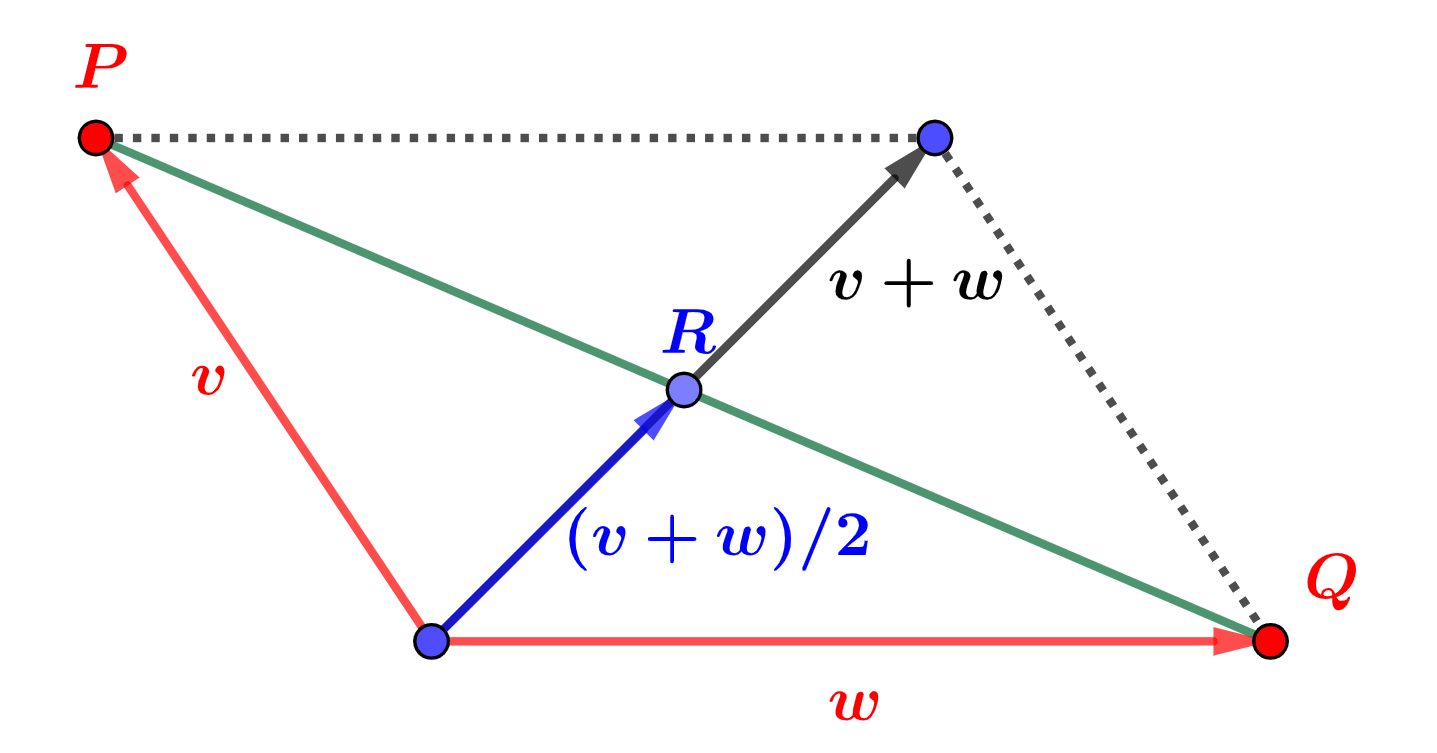
\includegraphics[scale=1]{img/ejercicios/1/10-a.png} 
\centering
\label{fig:1-10-a}
\end{figure}

\subsubsection*{1.10.b}
\label{subsubsec:1.10.b}
\addcontentsline{toc}{subsubsection}{\nameref{subsubsec:1.10.b}}

Sean los vectores $v$ y $w$ en función de sus puntos origen y extremo:

\begin{equation}
\begin{array}{ll}
& v = P-P_0 \\
& w = Q-Q_0
\end{array}
\end{equation}

Por definición:

\begin{equation}
u = v + t (w-v)
\end{equation}

Expresando $v$ y $w$ en función de sus puntos extremos:

\begin{subequations}
\begin{align}
& u = P - P_0 + t (Q - Q_0 - P + P_0) \\
& u = P - P_0 + t Q - t Q_0 - t P + t P_0 \\
& u = \underbrace{ P + t (Q-P) }_{\text{extremo } R} - \underbrace{ P_0 + t (Q_0 - P_0) }_{\text{origen } R_0}
\end{align}
\end{subequations}

La distancia entre el extremo del vector $u$, o sea el punto $R$, y el punto $P$, es entonces:

\begin{equation}
||R-P|| = ||t (Q-P)|| = |t| ||Q - P|| \overset{0<t<1}{=} t ||Q-P||
\end{equation}

Ahora bien, los puntos $Q$ y $P$ son los extremos de $w$ y $v$. La distancia entre los extremos equivale a la norma del vector resta: $||Q-P|| = ||w-v||$, con lo que se llega al resultado deseado:

\begin{equation}
||R-P|| = t ||w-v||, \text{ con } R = P + t (Q-P)
\end{equation}

Visualmente, se tiene la situación de la figura \ref{fig:1-10-b}.  

\begin{figure}[ht]
\caption{$t ||w-v||$}
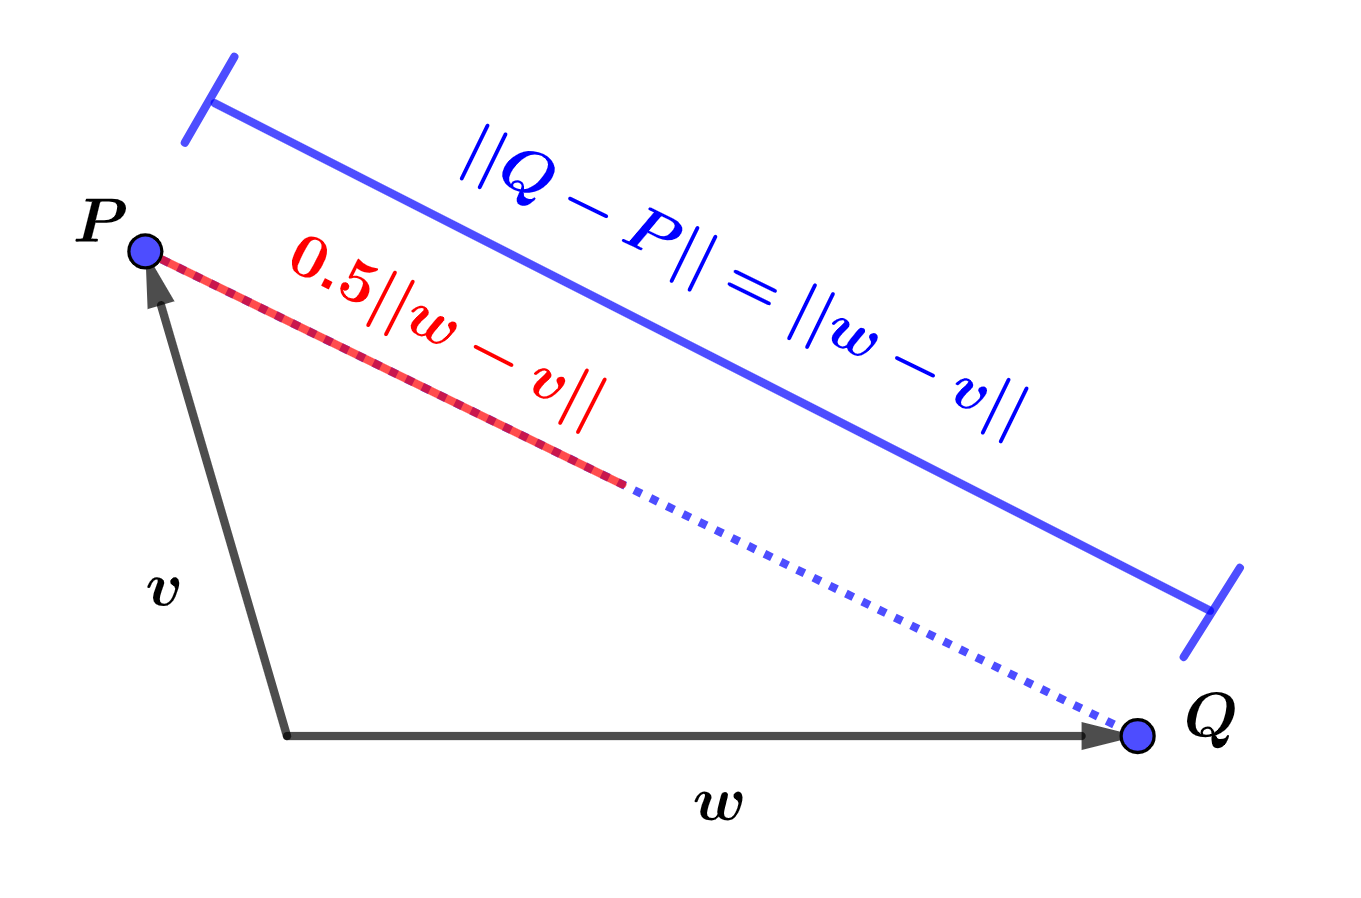
\includegraphics[scale=1]{img/ejercicios/1/10-b.png} 
\centering
\label{fig:1-10-b}
\end{figure}

Al variar $t$ entre 0 y 1, se está tomando un segmento proporcional del vector resta. 

\hrule
\vspace{10 pt}

\subsection*{1.11}
\label{subsec:1.11}
\addcontentsline{toc}{subsection}{\nameref{subsec:1.11}}

\textbf{Describir mediante un gráfico las regiones planas dadas por las siguientes inecuaciones:}

\begin{enumerate}[(a)]
\bfseries
\item $x + y \leq 1$

\item $x - y \geq 1, x \geq 2$

\item $x^2 + y^2 \geq 1, x \geq 0$

\item $y - x^2 \geq 0, y \geq 2$

\item $y - 2 - x^2 \geq 0, y \geq 2$

\item $y - x^2 + 2x \geq 0, y \geq 2$

\item $x y \geq 1$

\item $x^2 - y^2 \geq 1$

\item $x \leq e^{-y}$

\item $x^2 + y^2/4 \leq 16$

\item $x^2 - 2x + y^2/4 - y \leq 16$

\item $y < \ln(x), x > 0$

\item $y > e^x + e^{-x}$

\item $\sin(x) < 1/2$

\item $\tan(x) < 1$
\end{enumerate}
\hrule

\subsubsection*{1.11.a}
\label{subsubsec:1.11.a}
\addcontentsline{toc}{subsubsection}{\nameref{subsubsec:1.11.a}}

Con inecuaciones lineales, lo más directo es ``despejar'' $y$, graficar la función del caso $=$, y ver cuál región de las delimitadas por la curva es la de interés. En este caso:

\begin{equation}
x + y \leq 1 \Leftrightarrow y \leq -x + 1
\end{equation}

\begin{figure}[ht]
\caption{\textbf{11-a)} $y \leq -x + 1$}
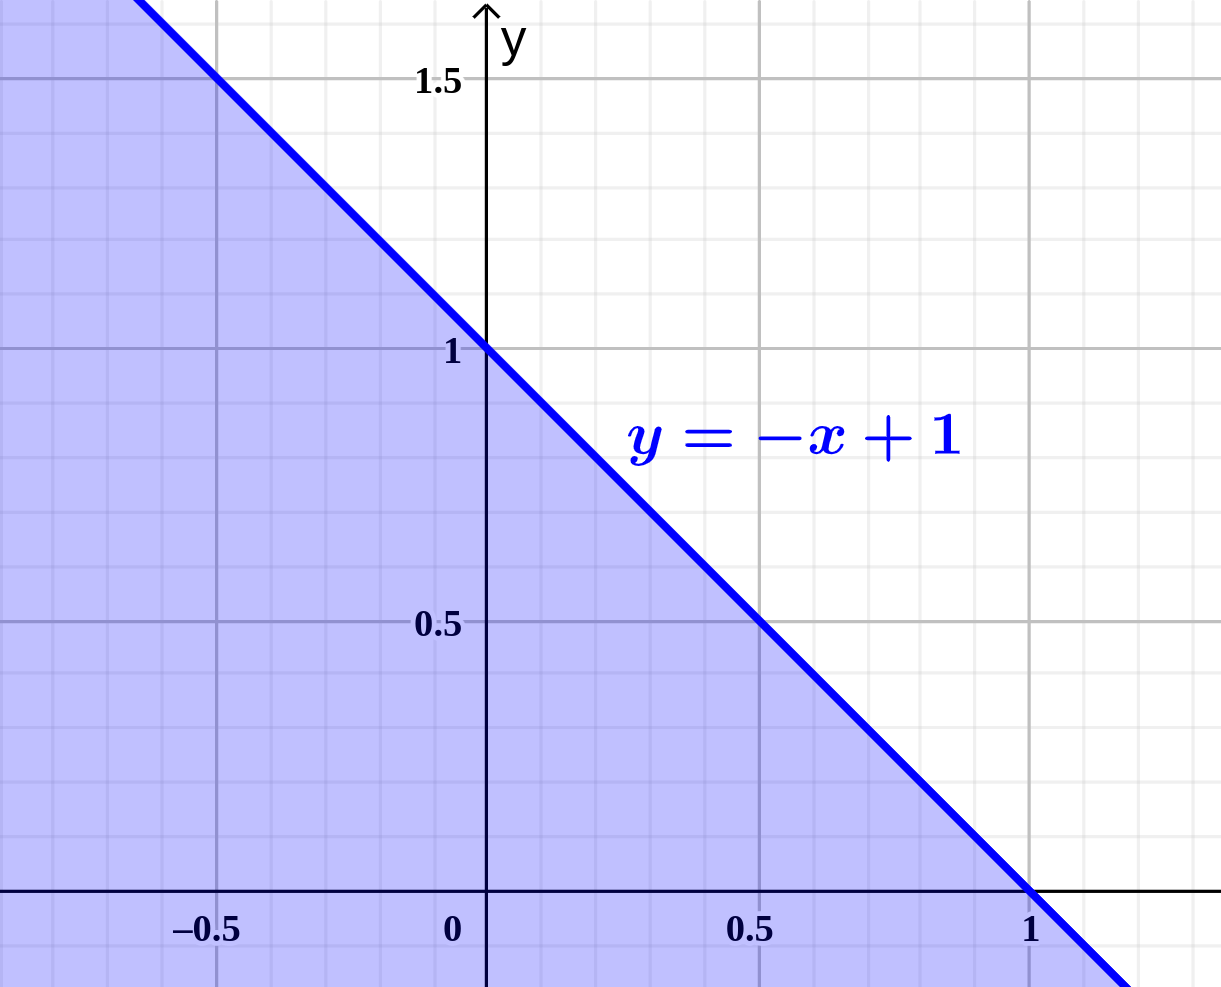
\includegraphics[scale=2.75]{img/ejercicios/1/11-a.png} 
\centering
\label{fig:1-11-a}
\end{figure}

Si hay dudas sobre cuál es la región, un método es evaluar un punto $(x,y)$ de una región y ver si satisface la inecuación. Por ejemplo, en este caso, $(0,0) \Rightarrow 0 \leq 1$ y por ende pertenece, y la región es la que está debajo de la recta. Ver figura \ref{fig:1-11-a}.

\subsubsection*{1.11.b}
\label{subsubsec:1.11.b}
\addcontentsline{toc}{subsubsection}{\nameref{subsubsec:1.11.b}}

En este caso, es necesario recordar que multiplicar una inecuación por un número negativo miembro a miembro invierte el sentido de la misma. Por otro lado, en este caso se tiene la intersección de dos regiones. Ver figura \ref{fig:1-11-b}.

\begin{equation}
x - y \geq 1 \Leftrightarrow -y \geq -x + 1 \Leftrightarrow y \leq x - 1
\end{equation}

\begin{figure}[ht]
\caption{\textbf{11-b)} $y \leq x - 1, x \geq 2$}
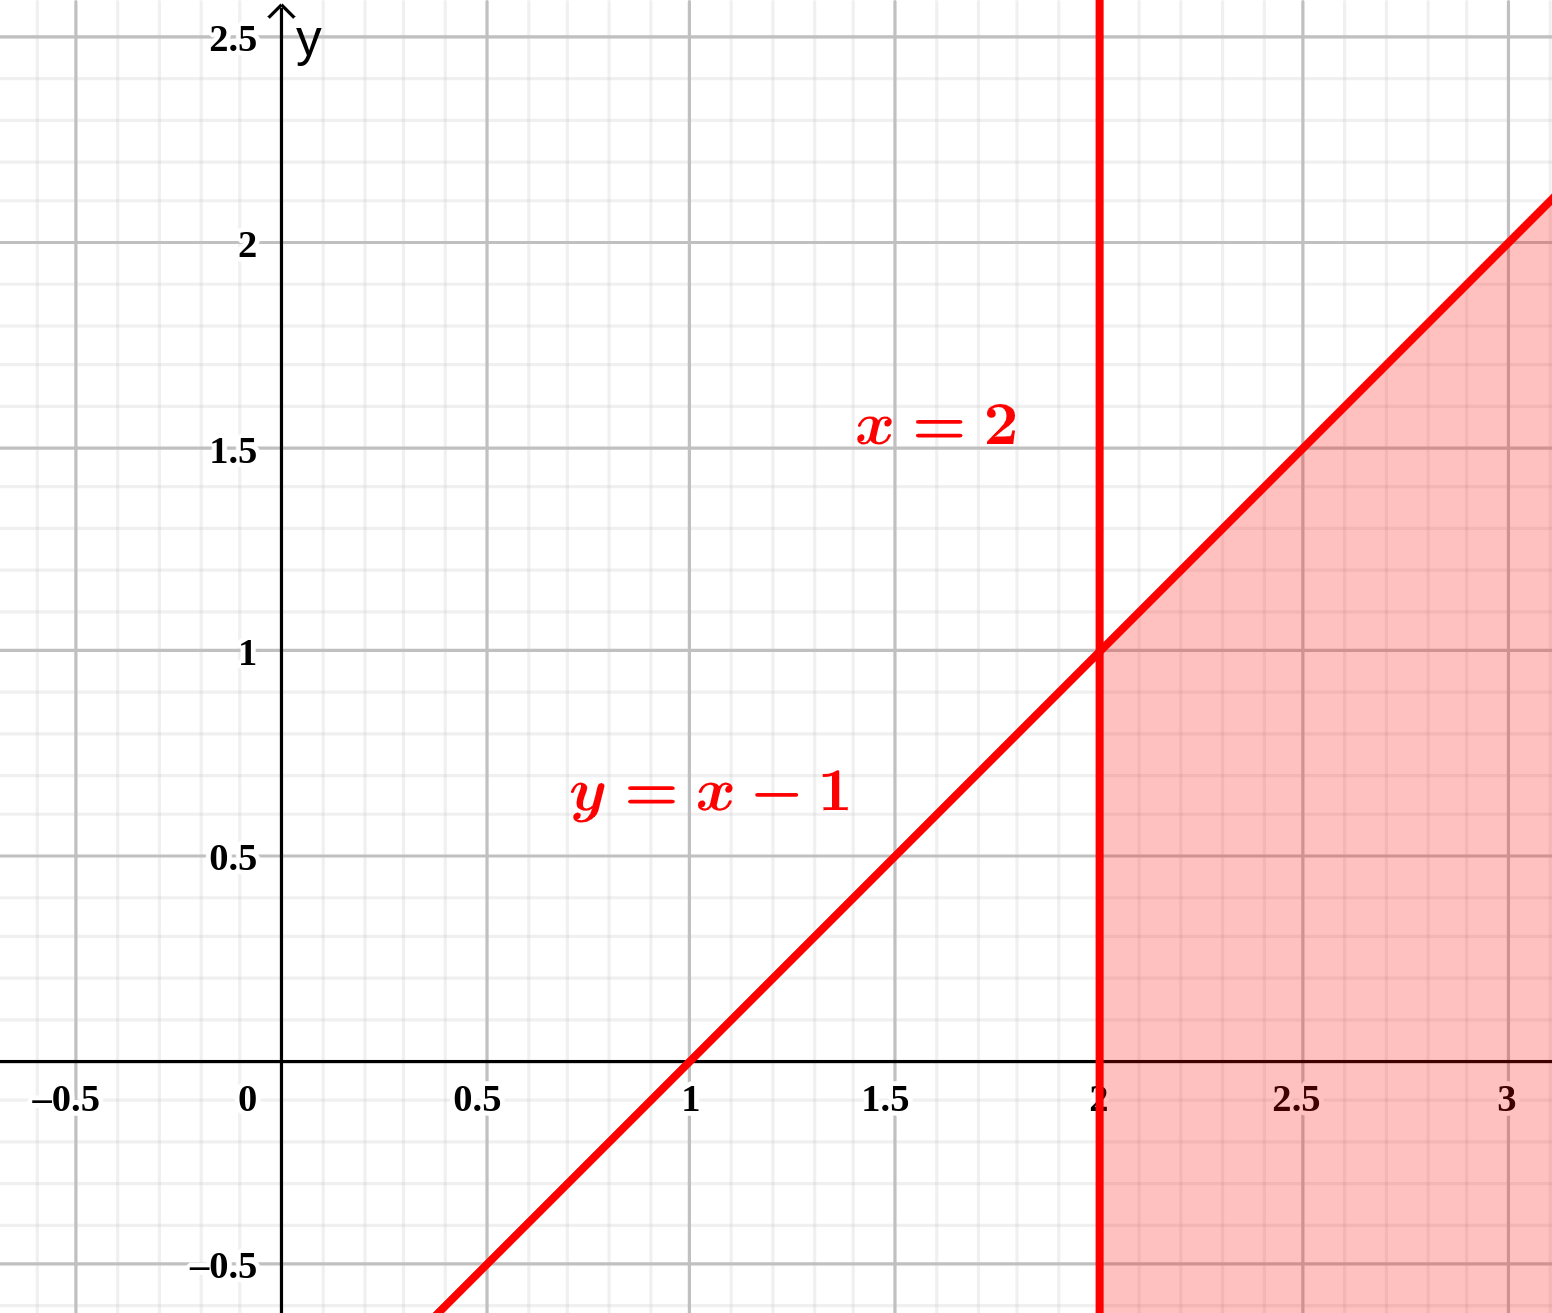
\includegraphics[scale=1.75]{img/ejercicios/1/11-b.png} 
\centering
\label{fig:1-11-b}
\end{figure}

\subsubsection*{1.11.c}
\label{subsubsec:1.11.c}
\addcontentsline{toc}{subsubsection}{\nameref{subsubsec:1.11.c}}

En este caso, hay que reconocer que $x^2 + y^2 \geq 1$ es el exterior de un círculo de radio 1 centrado en el origen. Con la condición extra $x >= 0$, se toma el semiplano positivo de dicho exterior. Ver figura \ref{fig:1-11-c}.

\begin{figure}[ht]
\caption{\textbf{11-c)} $x^2 + y^2 \geq 1, x \geq 0$}
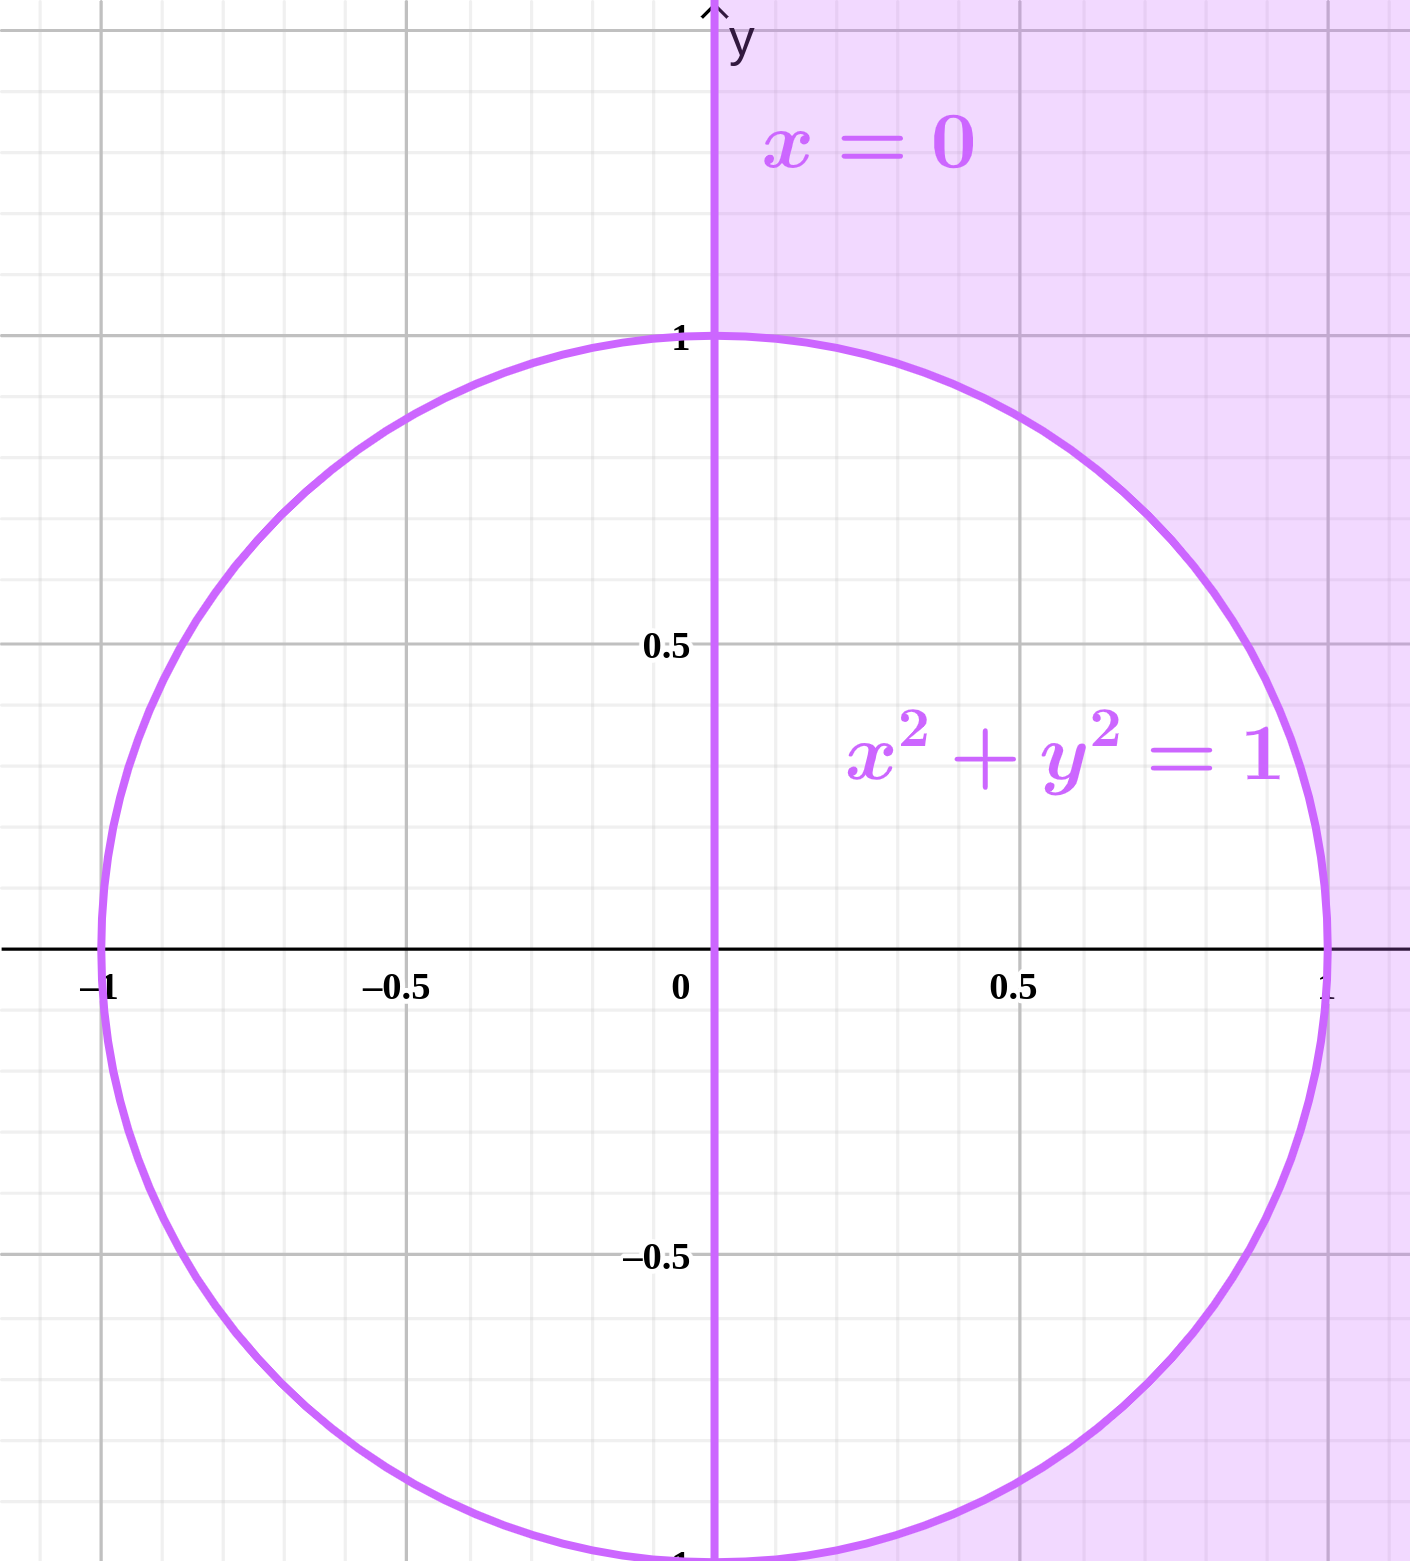
\includegraphics[scale=1.85]{img/ejercicios/1/11-c.png} 
\centering
\label{fig:1-11-c}
\end{figure}

\subsubsection*{1.11.d}
\label{subsubsec:1.11.d}
\addcontentsline{toc}{subsubsection}{\nameref{subsubsec:1.11.d}}

En este caso, se tiene una parábola:

\begin{equation}
y - x^2 \geq 1 \Leftrightarrow y \geq x^2 + 1
\end{equation}

En este caso, es trivial ver que el mínimo de la parábola está en $(0, 1)$, y es simétrica respecto al eje vertical de dicho punto (la recta $x = 0$). Nuevamente, la restricción $x \geq 0$ toma el semiplano positivo de la región sobre la curva. Ver figura \ref{fig:1-11-d}.

\begin{figure}[ht]
\caption{\textbf{11-d)} $y - x^2 \geq 1, x \geq 0$}
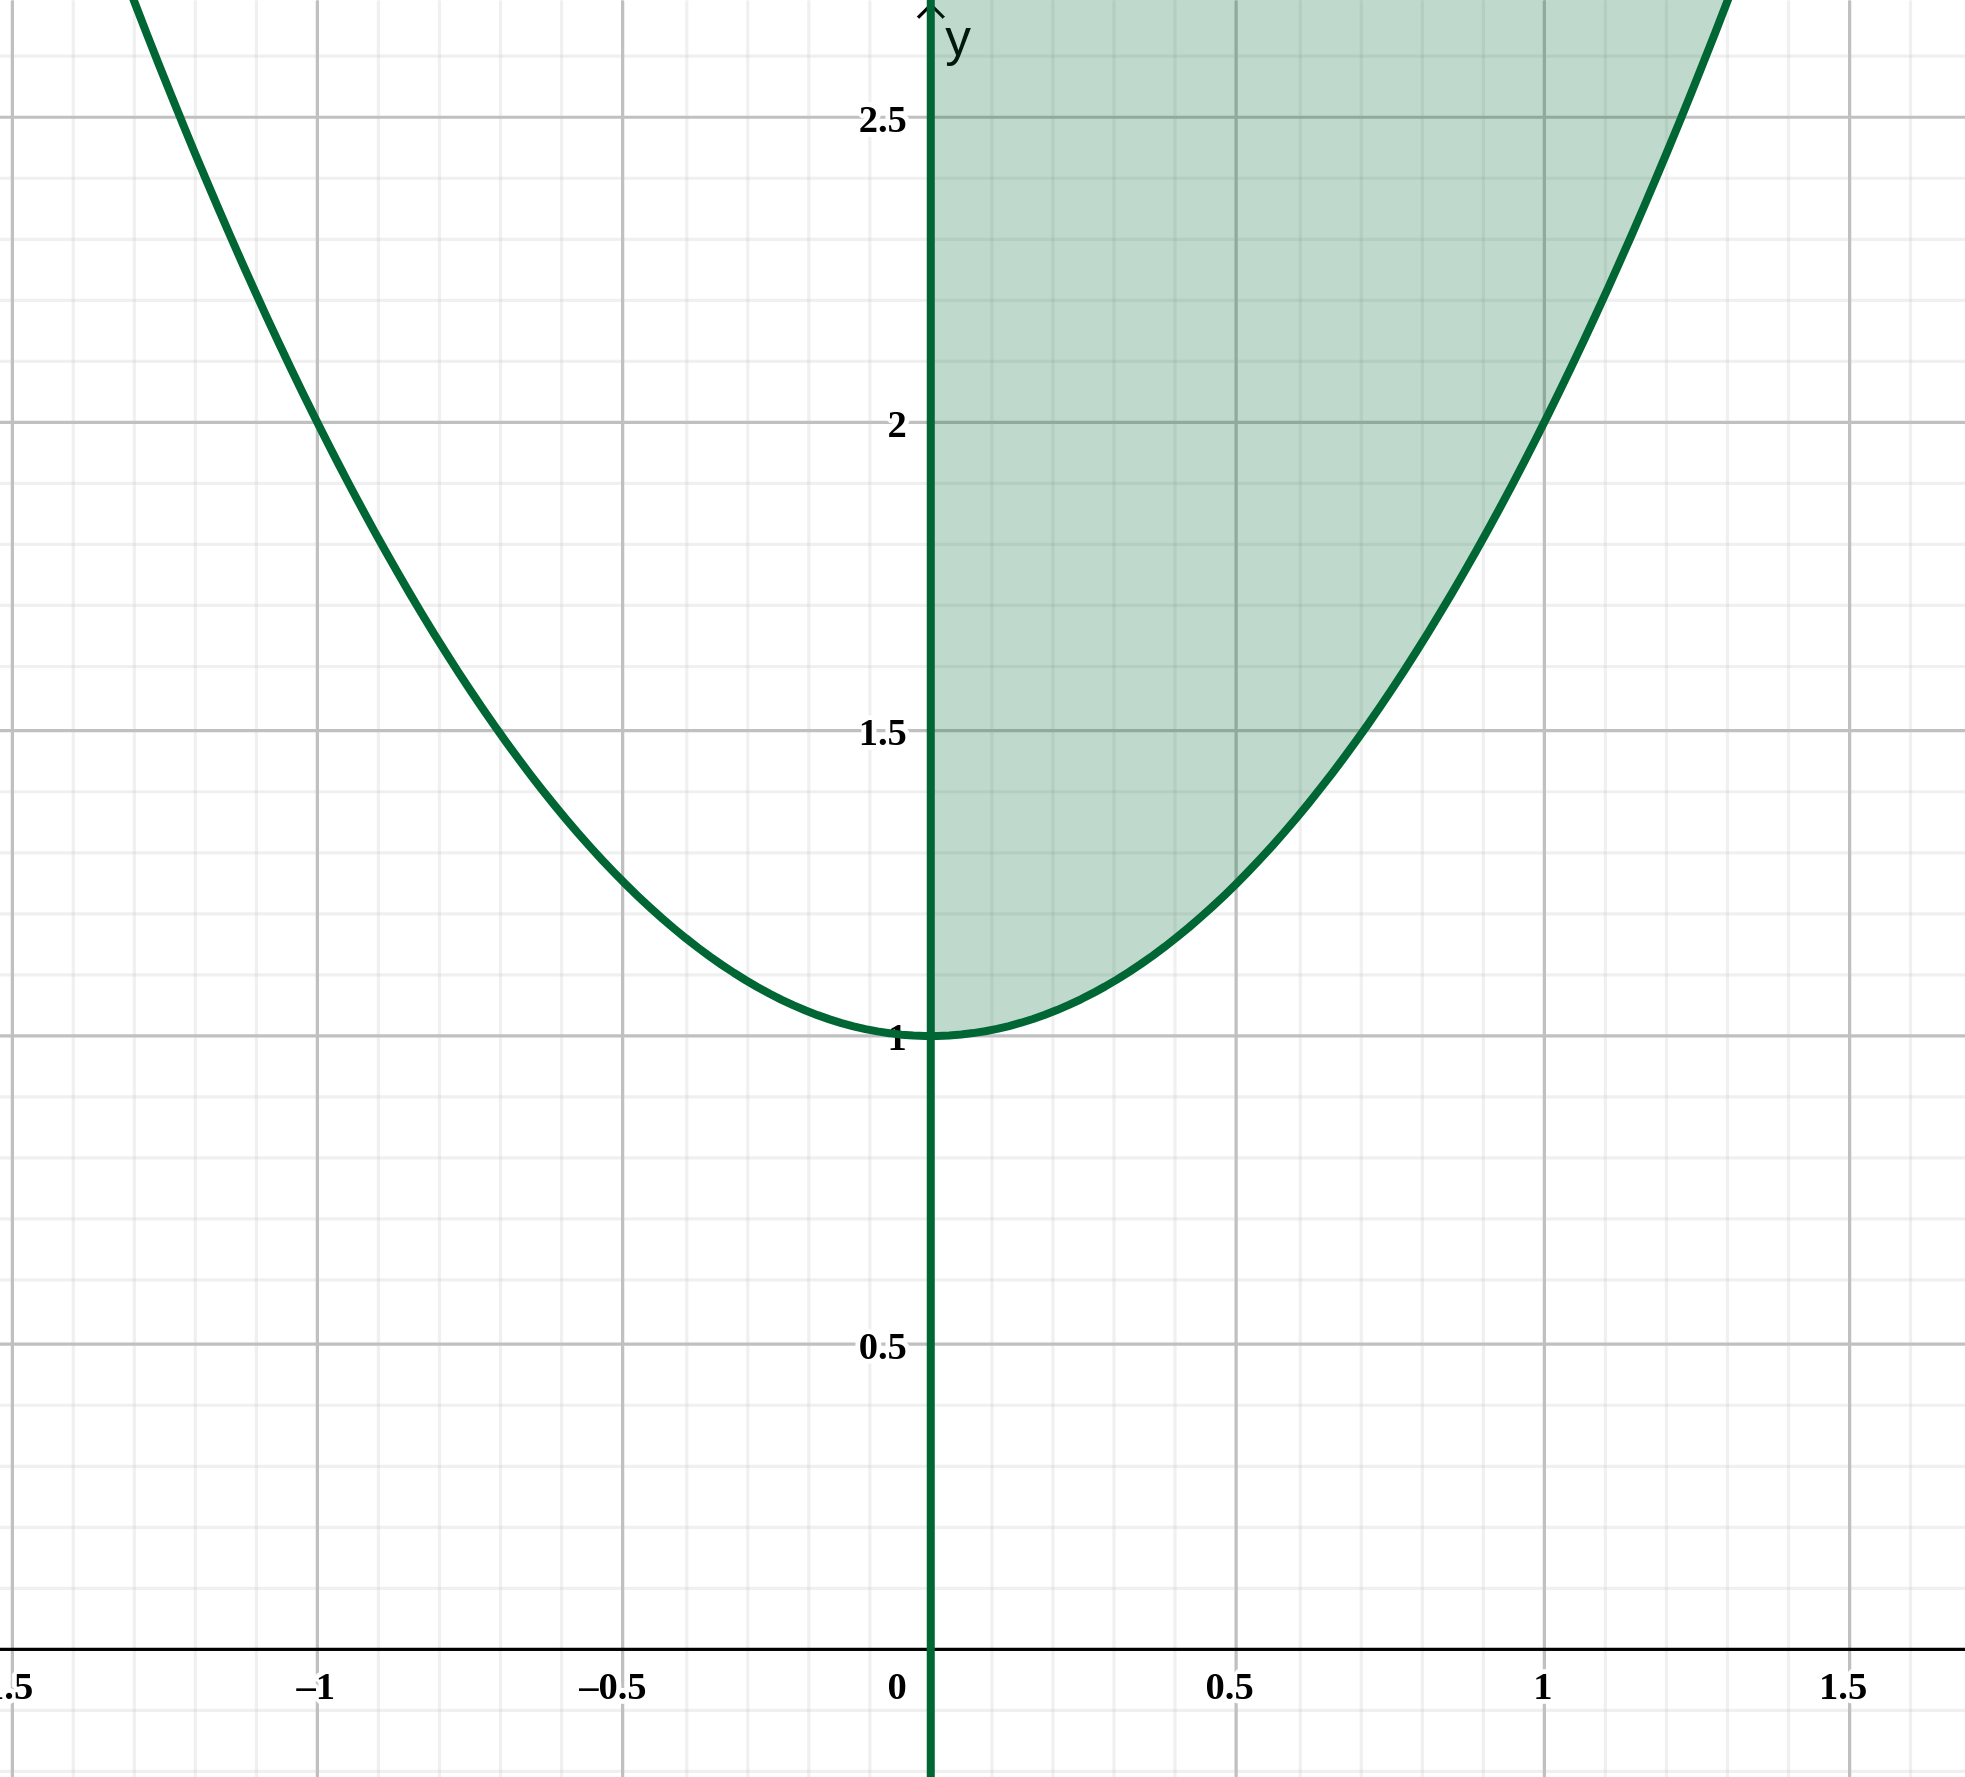
\includegraphics[scale=1.75]{img/ejercicios/1/11-d.png} 
\centering
\label{fig:1-11-d}
\end{figure}

\subsubsection*{1.11.e}
\label{subsubsec:1.11.e}
\addcontentsline{toc}{subsubsection}{\nameref{subsubsec:1.11.e}}

Análoga a la anterior, con la salvedad de que la restricción extra es sobre $y$. Ver figura \ref{fig:1-11-e}.

\begin{figure}[ht]
\caption{\textbf{11-e)} $y \geq x^2 + 2, y \geq 2$}
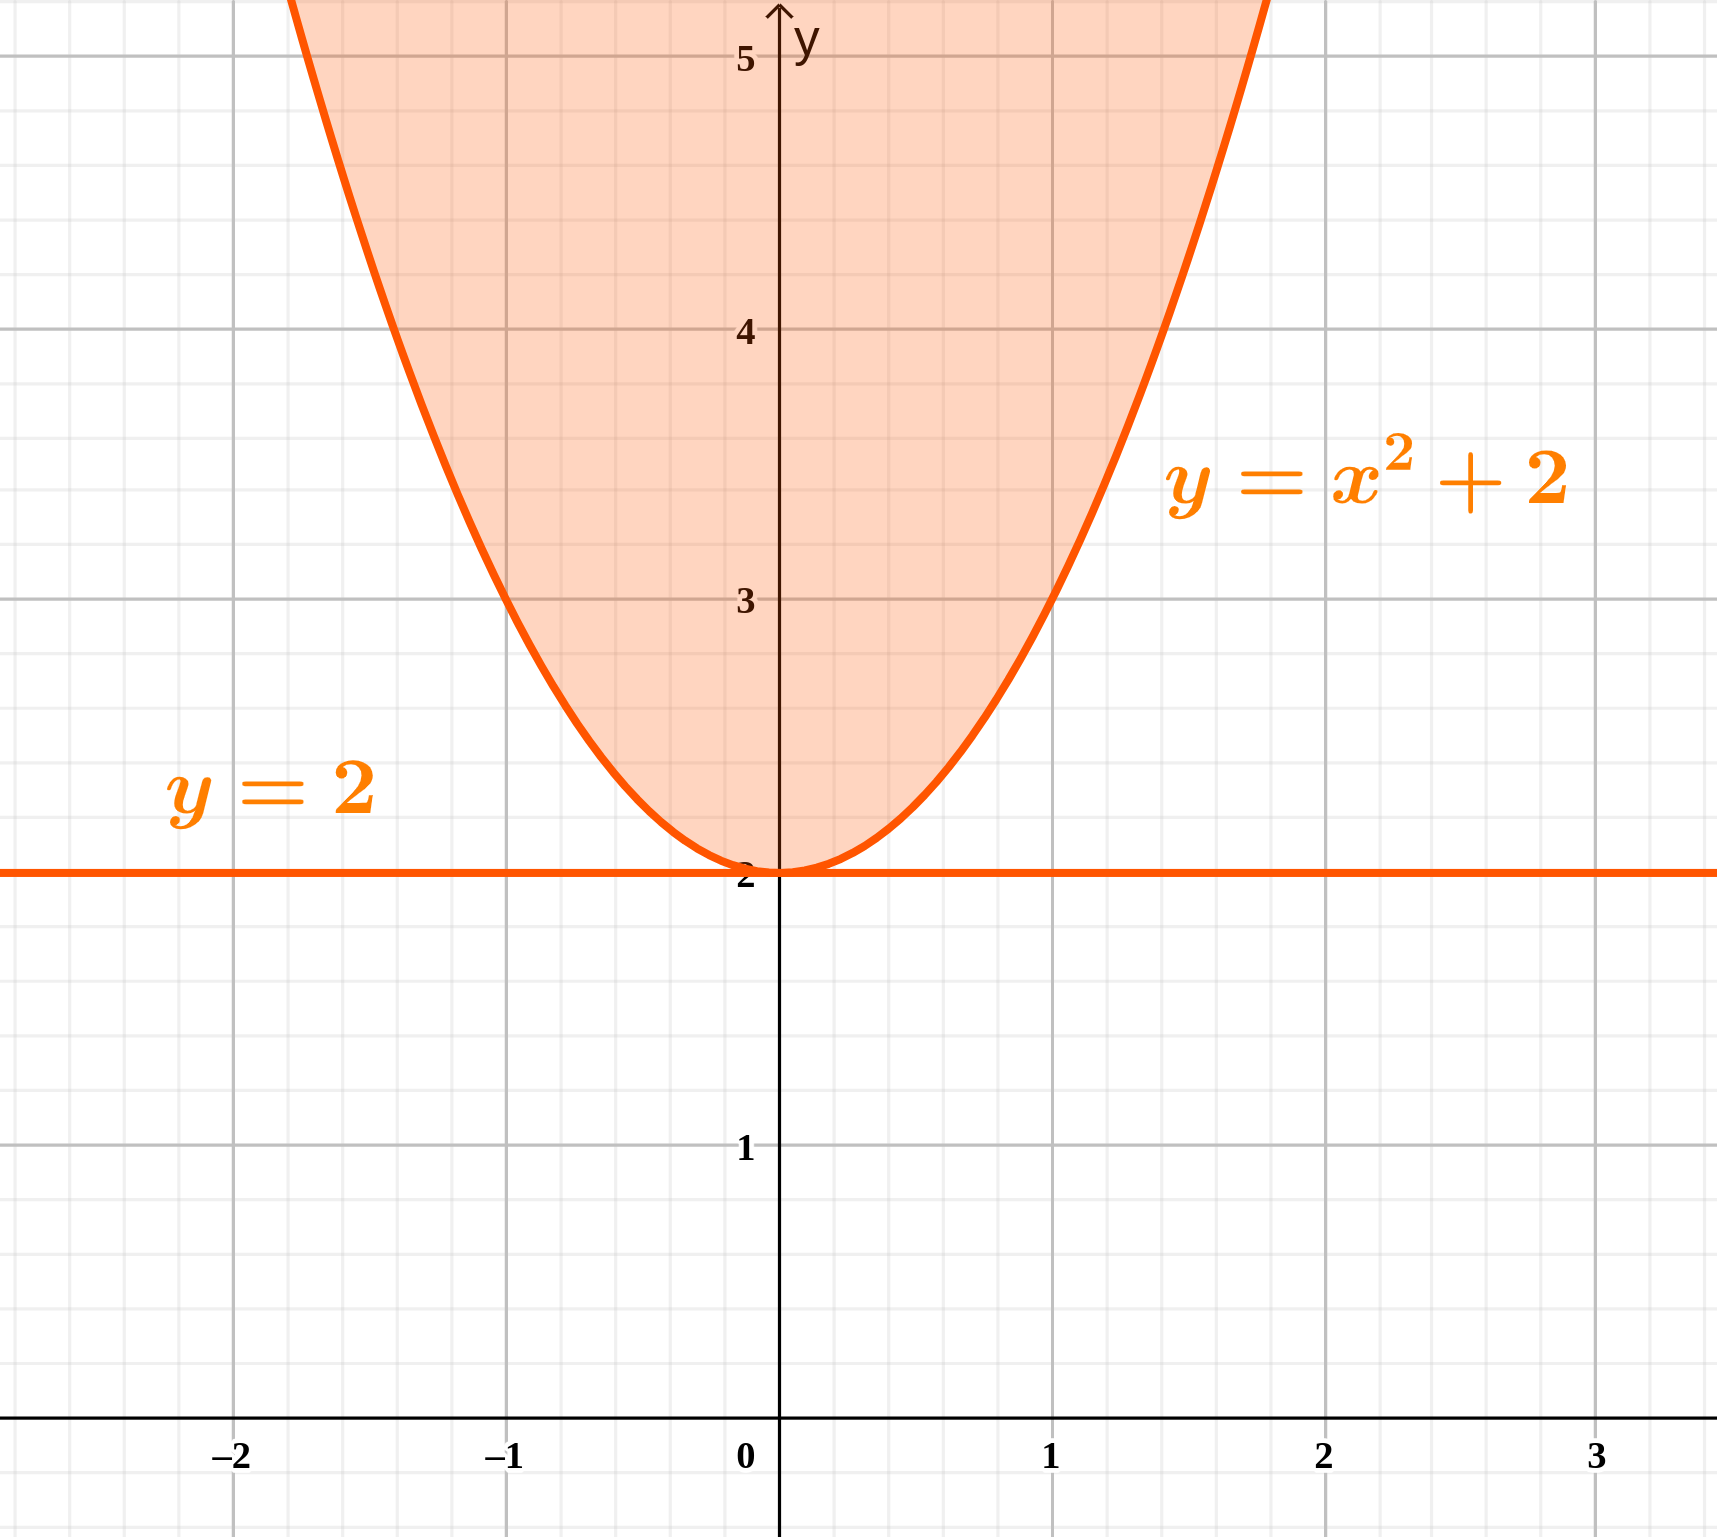
\includegraphics[scale=1.0]{img/ejercicios/1/11-e.png} 
\centering
\label{fig:1-11-e}
\end{figure}

\subsubsection*{1.11.f}
\label{subsubsec:1.11.f}
\addcontentsline{toc}{subsubsection}{\nameref{subsubsec:1.11.f}}

En este caso, para graficar la parábola conviene re-expresarla completando cuadrados en la variable $x$.

\begin{equation}
y \geq x^2 - 2x \Leftrightarrow y \geq (x-1)^2 - 1
\end{equation}

Esto indica que el vértice de la parábola está en el punto $(1, -1)$. Ver figura \ref{fig:1-11-f}.

\begin{figure}[ht]
\caption{\textbf{11-f)} $y \geq (x-1)^2 - 1, y \geq 2$}
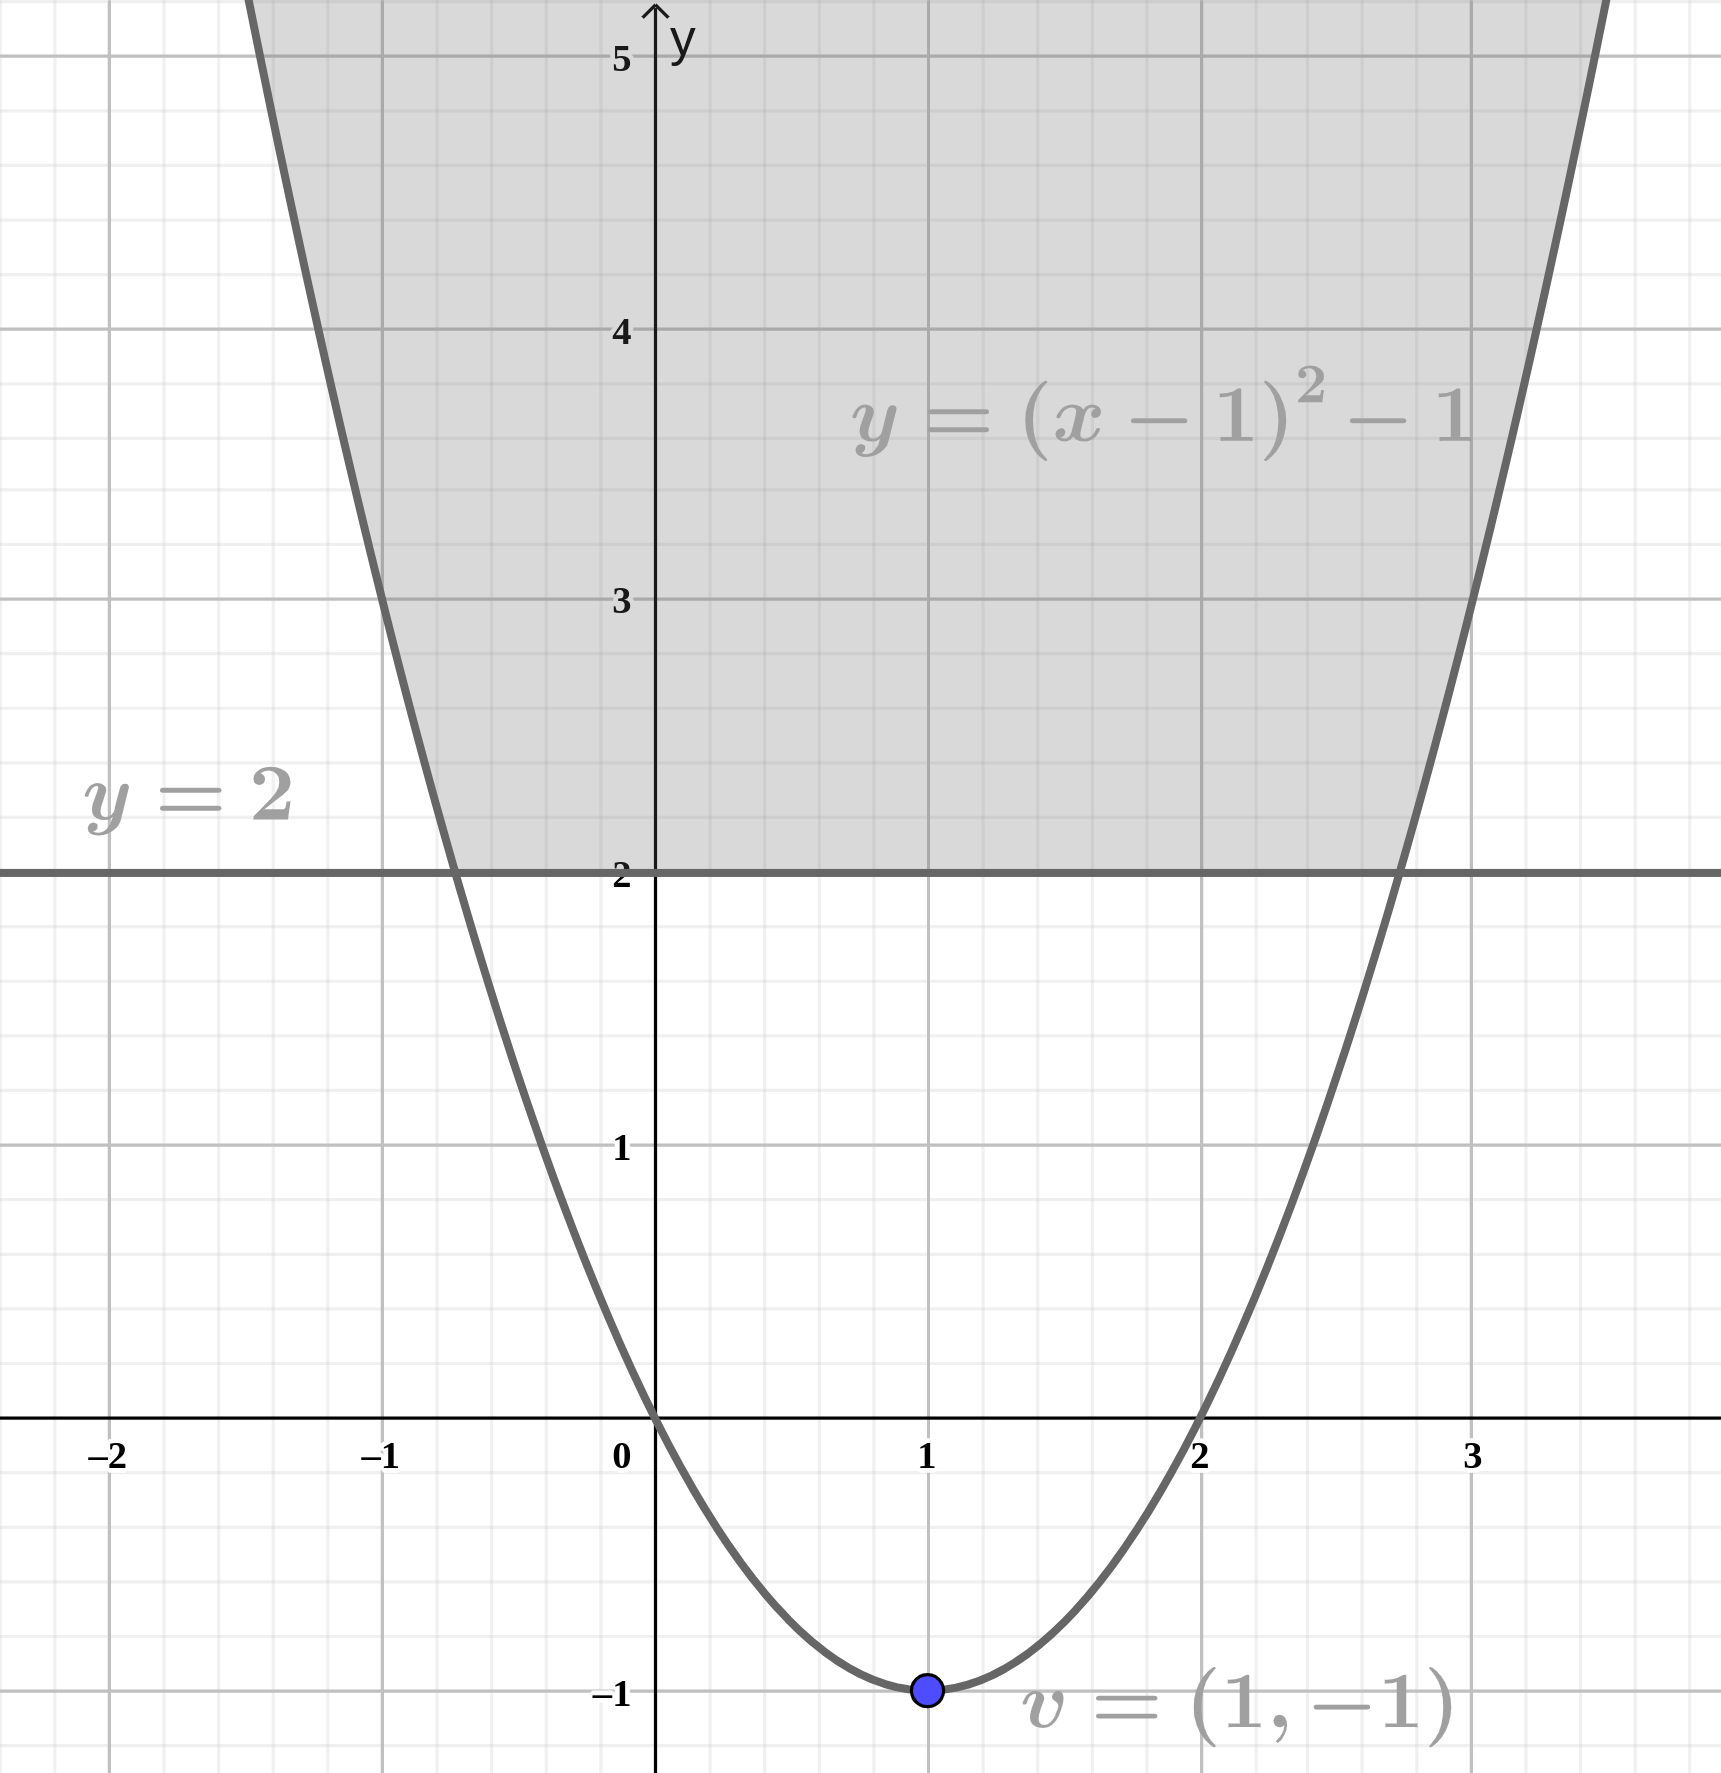
\includegraphics[scale=0.75]{img/ejercicios/1/11-f.png} 
\centering
\label{fig:1-11-f}
\end{figure}

\subsubsection*{1.11.g}
\label{subsubsec:1.11.g}
\addcontentsline{toc}{subsubsection}{\nameref{subsubsec:1.11.g}}

Este caso parece simple, porque directamente se tiene $y \geq \frac{1}{x}$ pero no lo es tanto, porque si $x$ es negativo, se invierte la desigualdad. Evaluando puntos en cada región en la desigualdad original, $x y \geq 1$, se puede aclarar la cuestión.

\begin{itemize}
\item Encima de la curva del semiplano positivo: $(1, 5) \Rightarrow 5 \geq 1$. Pertenece.
\item Debajo de la curva del semiplano positivo: $(1, -1) \Rightarrow -1 \geq 1$. No pertenece.
\item Encima de la curva del semiplano negativo: $(-1, 1) \Rightarrow -1 \geq 1$. No pertenece.
\item Debajo de la curva del semiplano negativo: $(-1, -5) \Rightarrow 5 \geq 1$. Pertenece.
\end{itemize}

Ver figura \ref{fig:1-11-g}.

\begin{figure}[ht]
\caption{\textbf{11-g)} $x y \geq 1$}
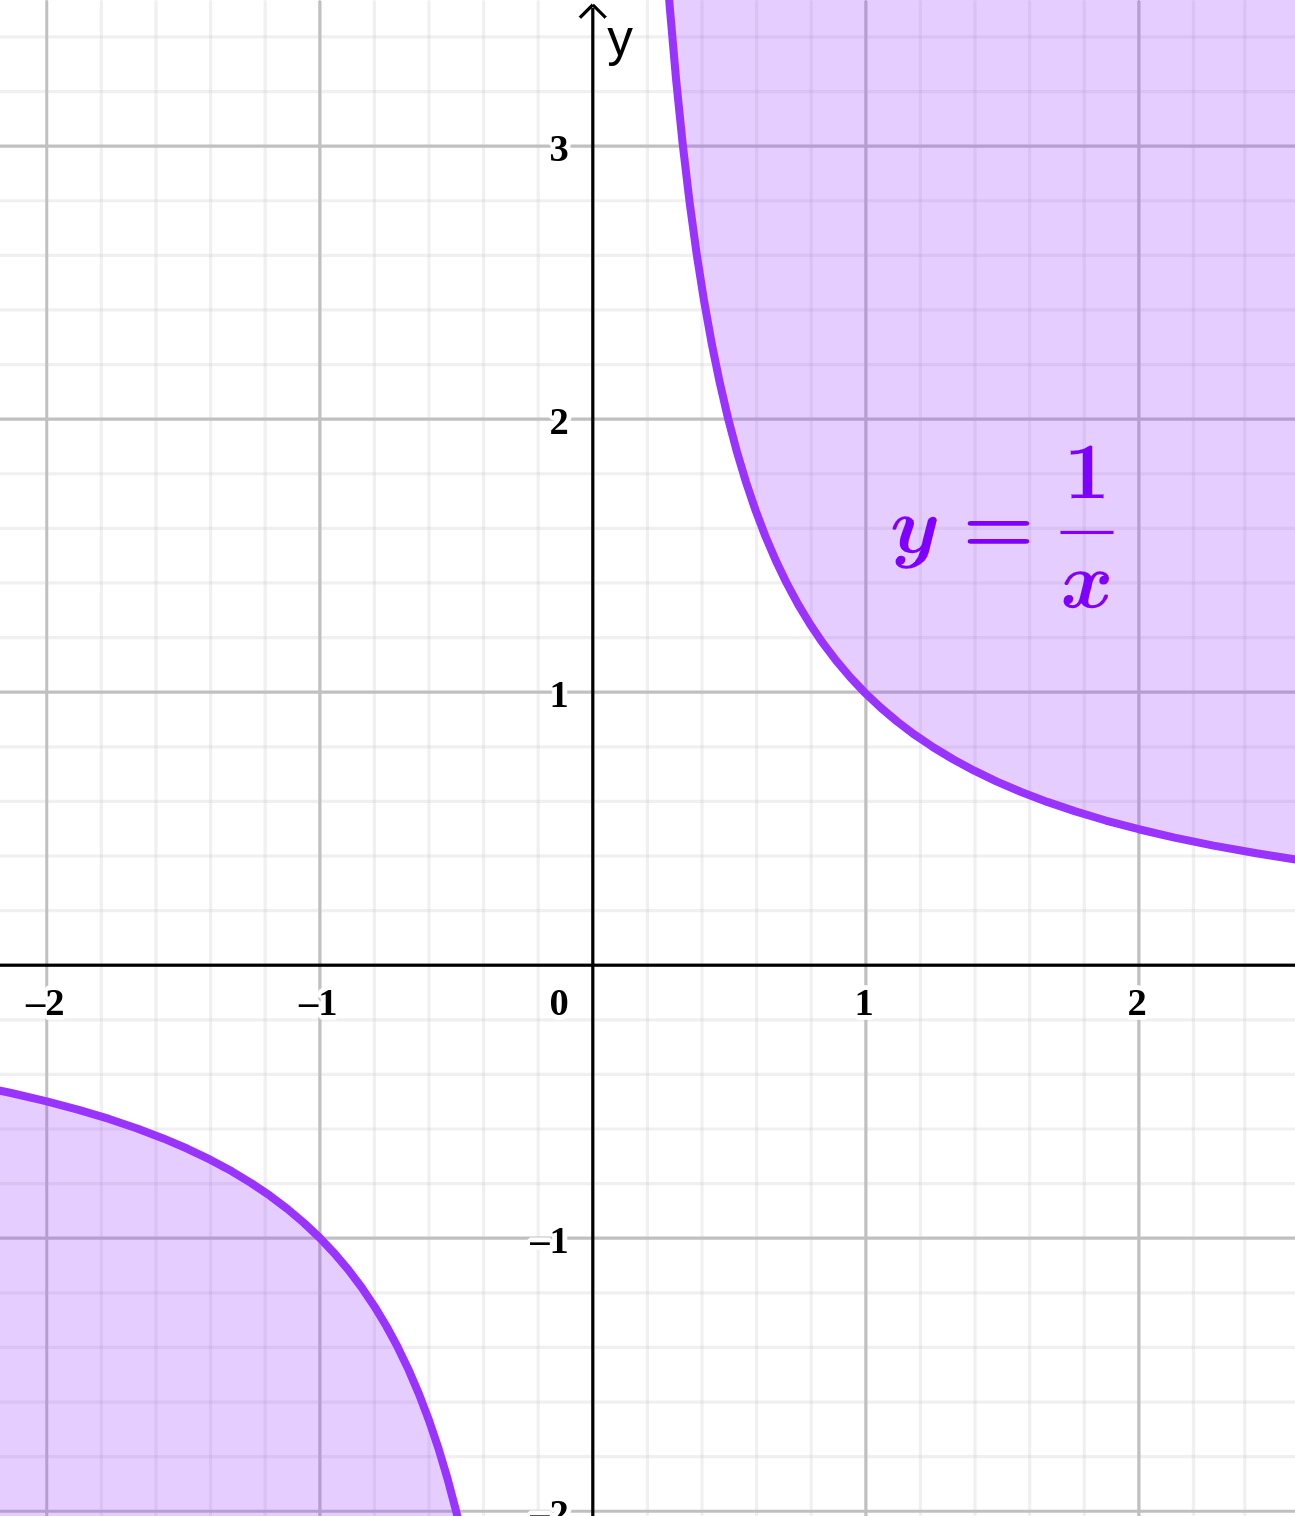
\includegraphics[scale=0.75]{img/ejercicios/1/11-g.png} 
\centering
\label{fig:1-11-g}
\end{figure}

\subsubsection*{1.11.h}
\label{subsubsec:1.11.h}
\addcontentsline{toc}{subsubsection}{\nameref{subsubsec:1.11.h}}

Recúerdese la ecuación general de una hipérbola:

\begin{equation}
\frac{(x-x_0)^2}{a^2} - \frac{(y-y_0)^2}{b^2} = 1
\end{equation}

Además, considérese que la hipérbola se grafica tomando como referencia un rectángulo de ancho $a$ y alto $b$, centrado en el punto $(x_0, y_0)$. Extendiendo las diagonales de dicho rectángulo como rectas infinitas, se tienen las asíntotas que definen las dos ramas de la hipérbola. Con esto en mente, en este caso particular, $a=1$, $b=1$, y el centro es el origen. Evaluando un punto de cada una de las tres regiones que esto genera en el plano, se obtiene:

\begin{itemize}
\item A la izquierda de la rama negativa: $(-2, 0) \Rightarrow 4 \geq 1$. Pertenece.
\item Entre las dos ramas: $(0, 0) \Rightarrow 0 \geq 1$. No pertenece.
\item A la derecha de la rama positiva: $(2, 0) \Rightarrow 4 \geq 1$. Pertenece.
\end{itemize}.

Ver figura \ref{fig:1-11-h}. Tener en cuenta que la curva es sólo la dibujada en rosa; el rectángulo y sus diagonales extendidas son sólo ayudas visuales para trazar el gráfico, y no pertenecen al mismo.

\begin{figure}[ht]
\caption{\textbf{11-h)} $x^2 - y^2 \geq 1$}
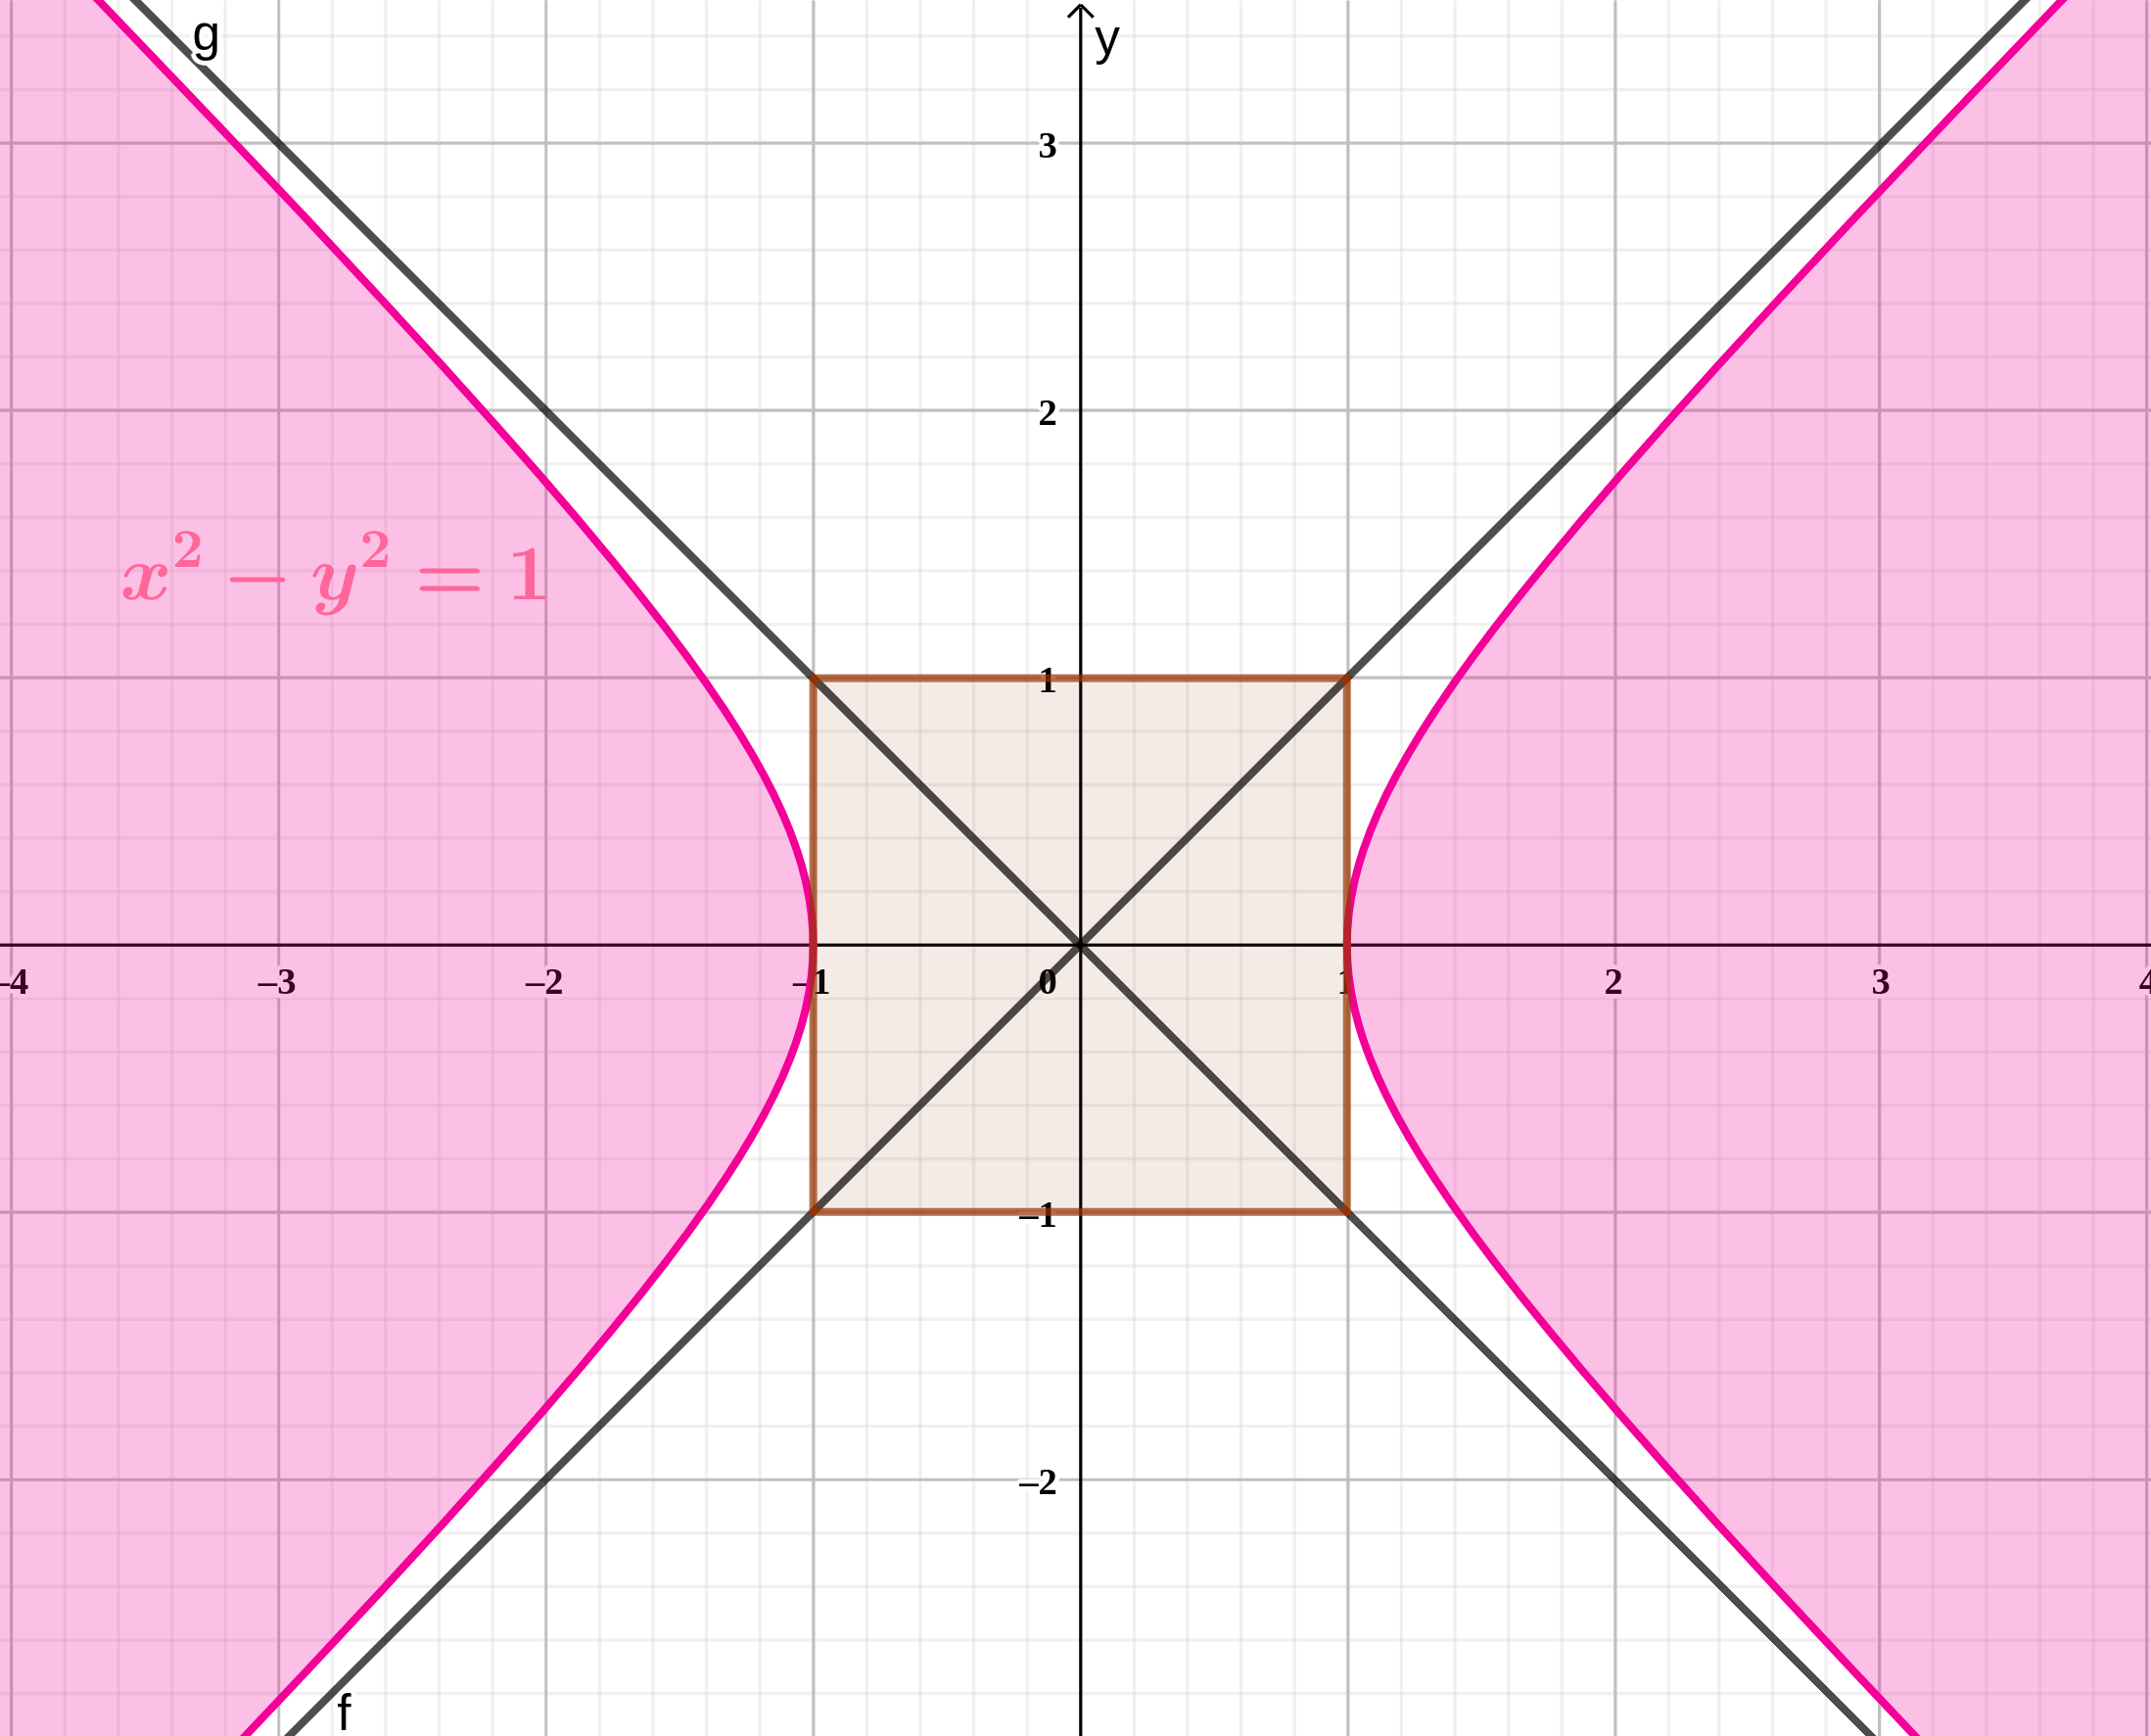
\includegraphics[scale=0.75]{img/ejercicios/1/11-h.png} 
\centering
\label{fig:1-11-h}
\end{figure}

\subsubsection*{1.11.i}
\label{subsubsec:1.11.i}
\addcontentsline{toc}{subsubsection}{\nameref{subsubsec:1.11.i}}

Una forma directa es graficar con los ejes $x$ e $y$ intercambiados. Una forma más larga, pero menos confusa es poner $y$ de un lado de la desigualdad. Tomando el logaritmo natural miembro a miembro:

\begin{equation}
\ln (x) \leq -y \Leftrightarrow -\ln(x) \geq y \Leftrightarrow y \leq -\ln(x)
\end{equation}

Para graficar $-\ln(x)$, basta con reflejar el conocido gráfico de $\ln(x)$ respecto al eje x. Ver figura \ref{fig:1-11-i}.

\begin{figure}[ht]
\caption{\textbf{11-i)} $y \leq -\ln(x)$}
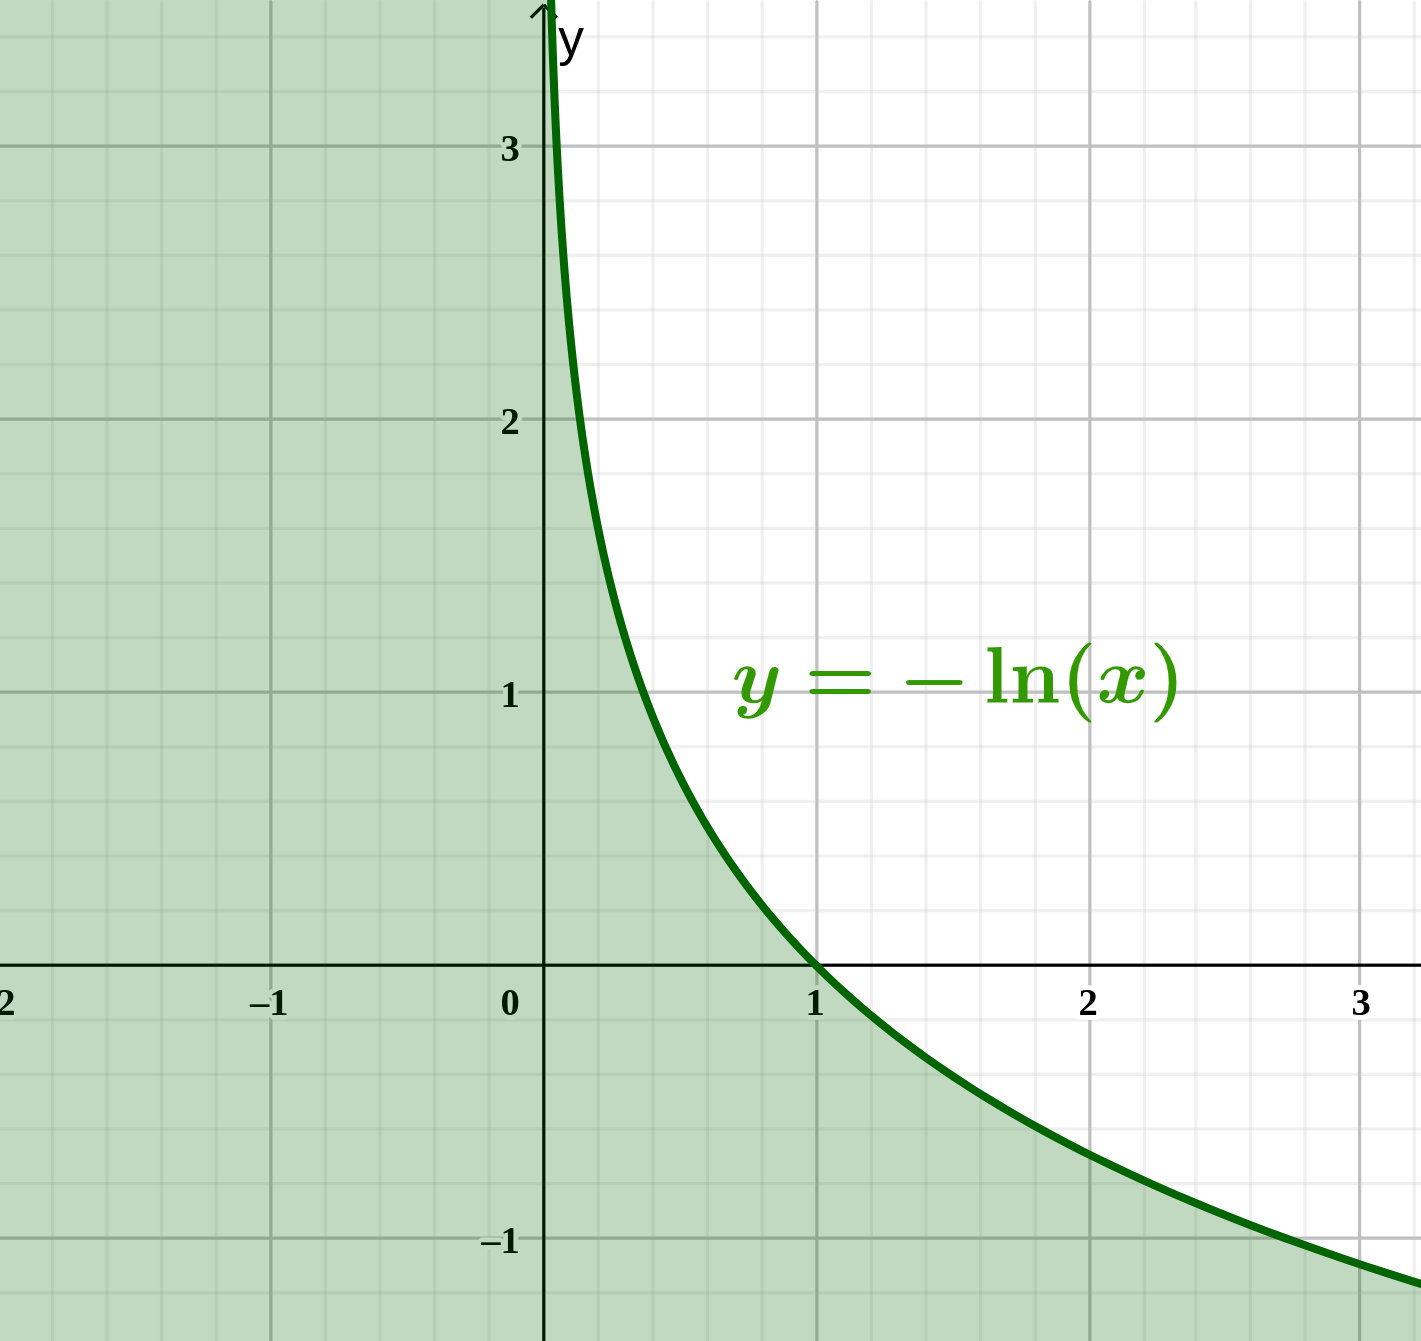
\includegraphics[scale=0.75]{img/ejercicios/1/11-i.png} 
\centering
\label{fig:1-11-i}
\end{figure}

\subsubsection*{1.11.j}
\label{subsubsec:1.11.j}
\addcontentsline{toc}{subsubsection}{\nameref{subsubsec:1.11.j}}

Recuérdese la forma general de una elipse:

\begin{equation}
\frac{(x-x_0)^2}{a^2} + \frac{(y-y_0)^2}{b^2} = 1
\end{equation}

Para relacionar la desigualdad con una elipse, hace falta una transformación, concretamente multiplicar por $\frac{1}{16}$ miembro a miembro (para que quede un 1 en el lado derecho):

\begin{equation}
\frac{x^2}{16} + \frac{y^2}{64} \leq 1
\end{equation}

Esta región es el interior de una elipse centrada en el origen de radio horizontal 4 y radio vertical 8. Ver figura \ref{fig:1-11-j}.

\begin{figure}[ht]
\caption{\textbf{11-j)} $\frac{x^2}{16} + \frac{y^2}{64} \leq 1$}
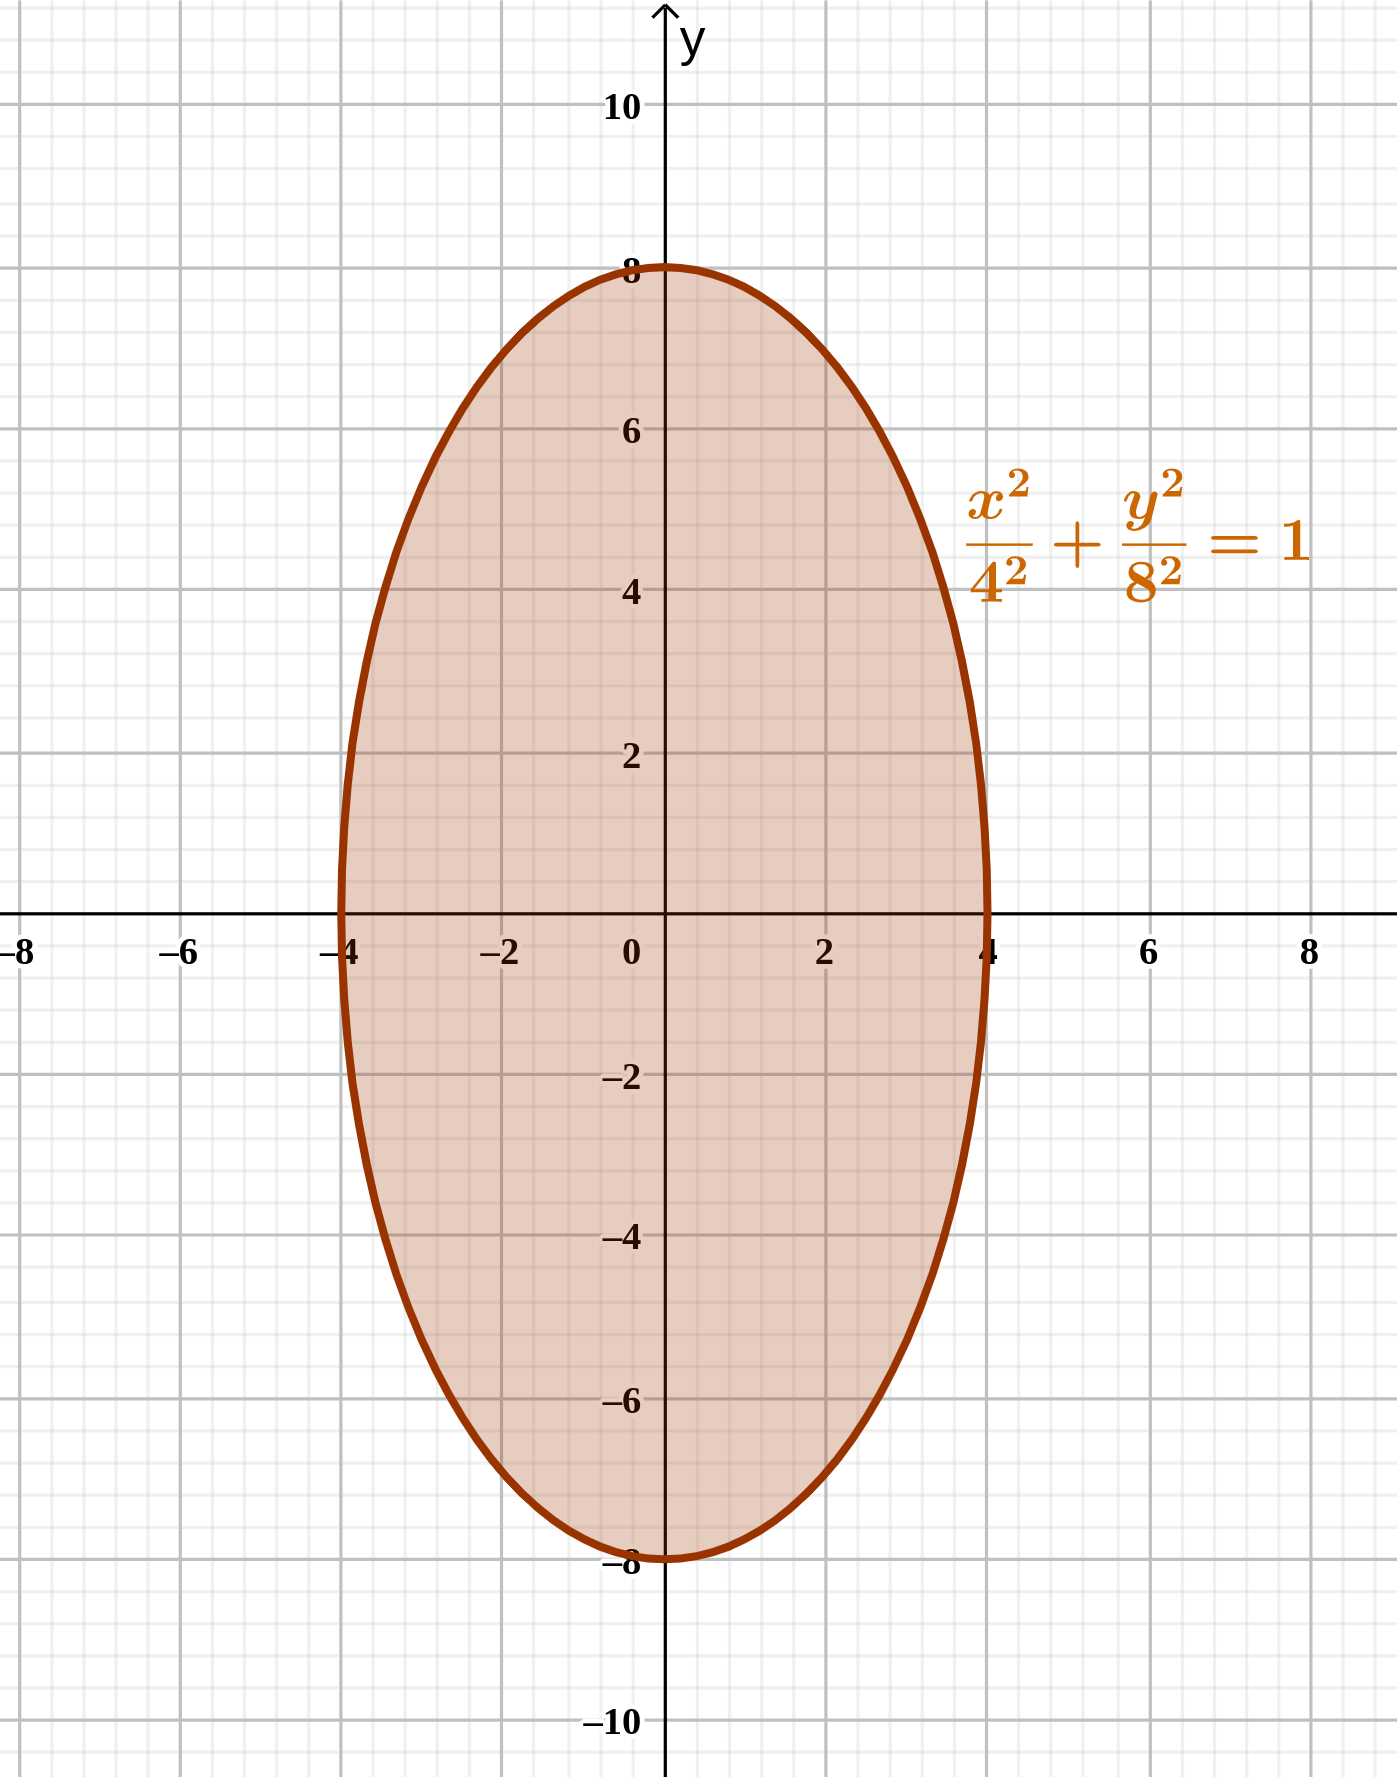
\includegraphics[scale=0.3]{img/ejercicios/1/11-j.png} 
\centering
\label{fig:1-11-j}
\end{figure}

\subsubsection*{1.11.k}
\label{subsubsec:1.11.k}
\addcontentsline{toc}{subsubsection}{\nameref{subsubsec:1.11.k}}

Para relacionar esta desigualdad con una elipse, es necesario completar cuadrados en $x$ y en $y$:

En x:

\begin{equation}
(x-1)^2 = x^2 -2x + 1 \Rightarrow x^2 - 2x = (x-1)^2 - 1
\end{equation}

En y:

\begin{equation}
\left (\frac{1}{2} y - 1 \right)^2 = \frac{1}{4}y^2 - y + 1 \Rightarrow \frac{y^2}{4} - y = (\frac{1}{2} y - 1)^2 - 1
\end{equation}

El próximo paso es acomodar la desigualdad para que cumpla la forma general de la elipse. Reemplazando con los cuadrados completos:

\begin{equation}
(x-1)^2 - 1 + \left( \frac{1}{2} y - 1 \right)^2 - 1 \leq 16
\end{equation}

Pasando las constantes a la derecha, y sacando factor común $\frac{1}{2}$ dentro del paréntesis de $y$:

\begin{equation}
(x-1)^2 + \left( \frac{1}{2} (y - 2) \right)^2 \leq 18
\end{equation}

Distribuyendo la potencia respecto al producto en $y$:

\begin{equation}
(x-1)^2 + \frac{(y-2)^2}{4} \leq 18
\end{equation}

El último paso es multiplicar todo por $\frac{1}{18}$.

\begin{equation}
\frac{(x-1)^2}{18} + \frac{(y-2)^2}{72} \leq 1
\end{equation}

De esta manera, la región buscada es el interior de una elipse centrada en el punto $(1, 2)$, con radio horizontal $\sqrt{18} \approx 4,24$ y radio vertical $\sqrt{72} \approx 8,48$. Ver figura \ref{fig:1-11-k}.

\begin{figure}[ht]
\caption{\textbf{11-k)} $\frac{(x-1)^2}{18} + \frac{(y-2)^2}{72} \leq 1$}
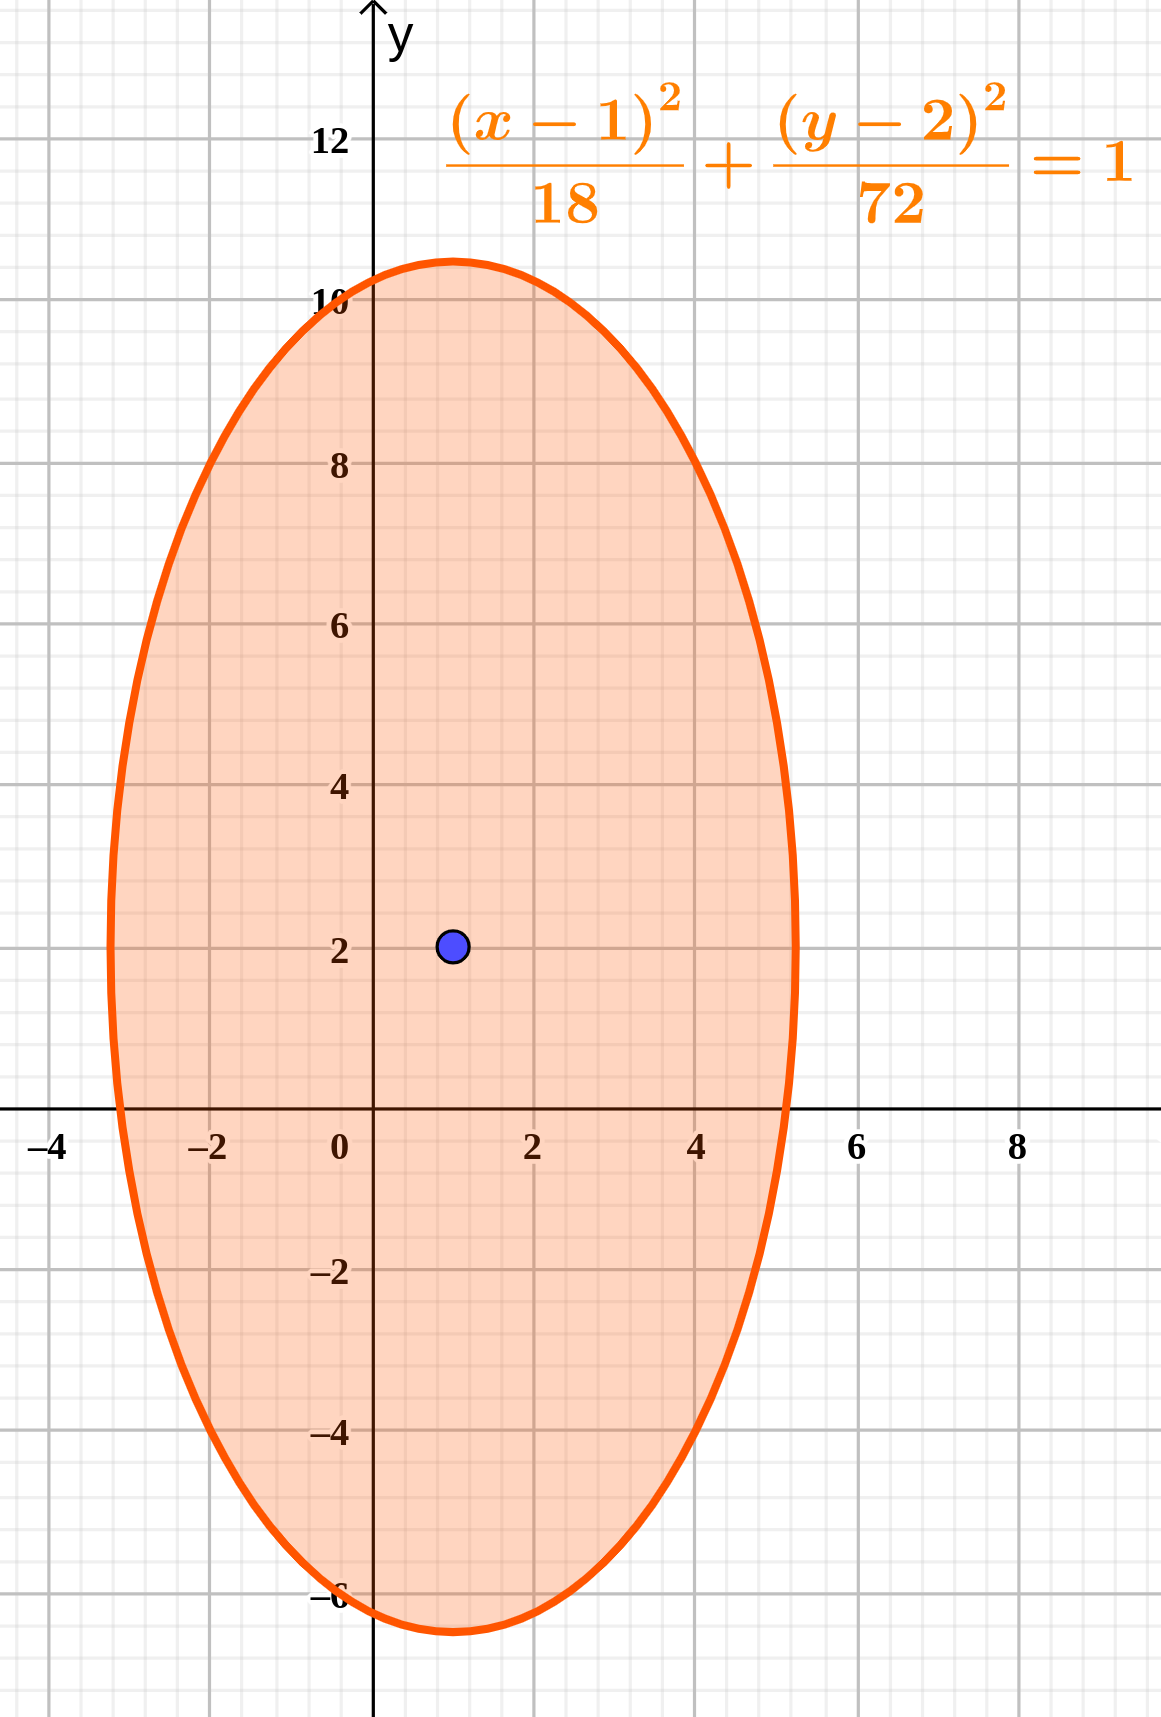
\includegraphics[scale=0.3]{img/ejercicios/1/11-k.png} 
\centering
\label{fig:1-11-k}
\end{figure}

\subsubsection*{1.11.l}
\label{subsubsec:1.11.l}
\addcontentsline{toc}{subsubsection}{\nameref{subsubsec:1.11.l}}

No es necesaria ninguna transformación para determinar que esta región es la inferior a la curva $y = ln(x)$. La condición $x > 0$ es redundante en este caso, porque el dominio de la función logaritmo son los reales mayores a cero. Ver figura \ref{fig:1-11-l}.

\begin{figure}[ht]
\caption{\textbf{11-l)} $y < \ln(x), x > 0$}
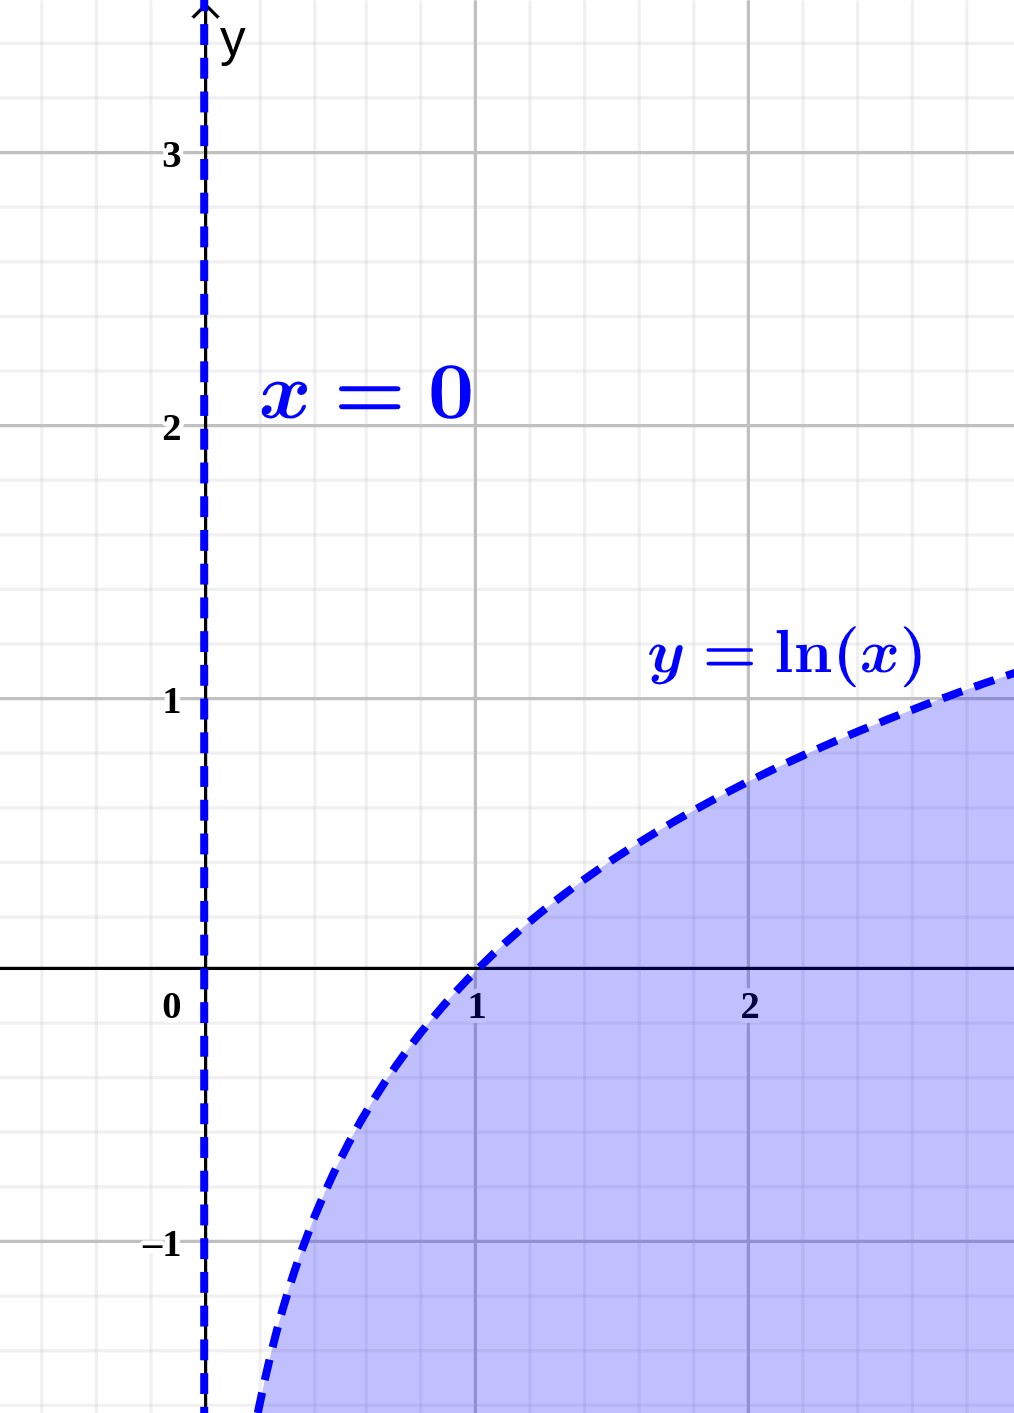
\includegraphics[scale=0.75]{img/ejercicios/1/11-l.png} 
\centering
\label{fig:1-11-l}
\end{figure}

\subsubsection*{1.11.m}
\label{subsubsec:1.11.m}
\addcontentsline{toc}{subsubsection}{\nameref{subsubsec:1.11.m}}

La clave es visualizar la función $y = e^x + e^{-x}$. Pensándola como la suma de una exponencial creciente y una decreciente, la simetría de ambas funciones genera una ``parábola exponencial'' (no es realmente parábola porque su tasa de crecimiento no es cuadrática, es exponencial). Dicha curva tiene su mínimo en $(0, 2)$. Ver figura \ref{fig:1-11-m}.

\begin{figure}[ht]
\caption{\textbf{11-m)} $y < e^x + e^{-x}$}
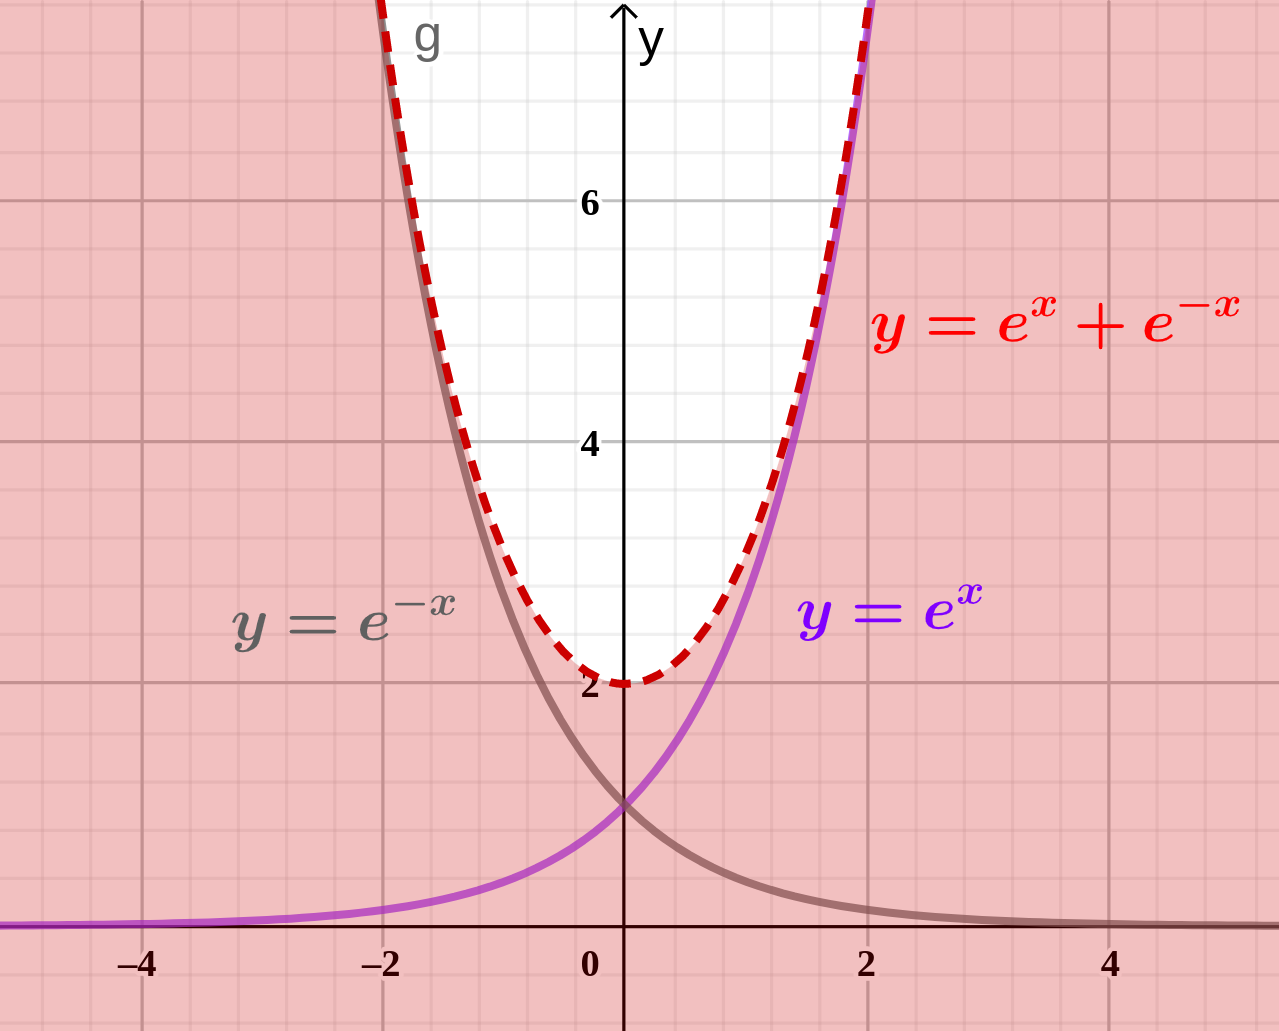
\includegraphics[scale=0.4]{img/ejercicios/1/11-m.png} 
\centering
\label{fig:1-11-m}
\end{figure}

\subsubsection*{1.11.n}
\label{subsubsec:1.11.n}
\addcontentsline{toc}{subsubsection}{\nameref{subsubsec:1.11.n}}

Tomando el arco seno miembro a miembro, y considerando la periodicidad del seno:

\begin{equation}
x < \arcsin \left( \frac{1}{2} \right) + 2 k \pi, k \in \Bbb Z
\end{equation}

Dado que $k \in \Bbb Z$, esta región es el conjunto vacío, porque equivale a pedir $x < -\infty$. Siempre habrá infinitos $k$ menores que impedirán que $x$ satisfaga la desigualdad.

\subsubsection*{1.11.ñ}
\label{subsubsec:1.11.ñ}
\addcontentsline{toc}{subsubsection}{\nameref{subsubsec:1.11.ñ}}

Algo similar ocurre en este caso, tomando en consideración que la función tangente es $\pi$-periódica. 

\begin{equation}
x < \arctan(1) + k \pi, k \in \Bbb Z
\end{equation}

Nuevamente, la región buscada es el conjunto vacío.

\hrule
\vspace{10 pt}

\subsection*{1.12}
\label{subsec:1.12}
\addcontentsline{toc}{subsection}{\nameref{subsec:1.12}}

\textbf{Describir mediante inecuaciones en coordenadas cartesianas las regiones planas dadas:}

\begin{enumerate}[(a)]
\bfseries
\item Interior del círculo centrado en $(0, 0)$ y de radio 2.

\item Cuadrado de lado 1 con lados paralelos a los ejes coordenados y vértice inferior izquierdo en $(1, 1)$.

\item Puntos por encima de la parábola de ecuación $y = 2x^2$.

\item Puntos interiores a la elipse de semiejes 2 y 4, paralelos a los ejes coordenados, centrada en $(0, 0)$.

\end{enumerate}
\hrule

\subsubsection*{1.12.a}
\label{subsubsec:1.12.a}
\addcontentsline{toc}{subsubsection}{\nameref{subsubsec:1.12.a}}

La forma general del interior de un círculo es:

\begin{equation}
(x-x_0)^2 + (y-y_0)^2 < r^2
\end{equation}

Para este caso, resulta $(x_0, y_0) = (0, 0)$ y $r=2$:

\begin{equation}
\tcboxmath[colback=orange!25!white,colframe=orange,title=1.12.a]
{ x^2 + y^2 < 4 }
\end{equation}

\subsubsection*{1.12.b}
\label{subsubsec:1.12.b}
\addcontentsline{toc}{subsubsection}{\nameref{subsubsec:1.12.b}}

Graficando, se ve inmediatamente. Ver figura \ref{fig:1-12-b}.

\begin{figure}[ht]
\caption{Cuadrado}
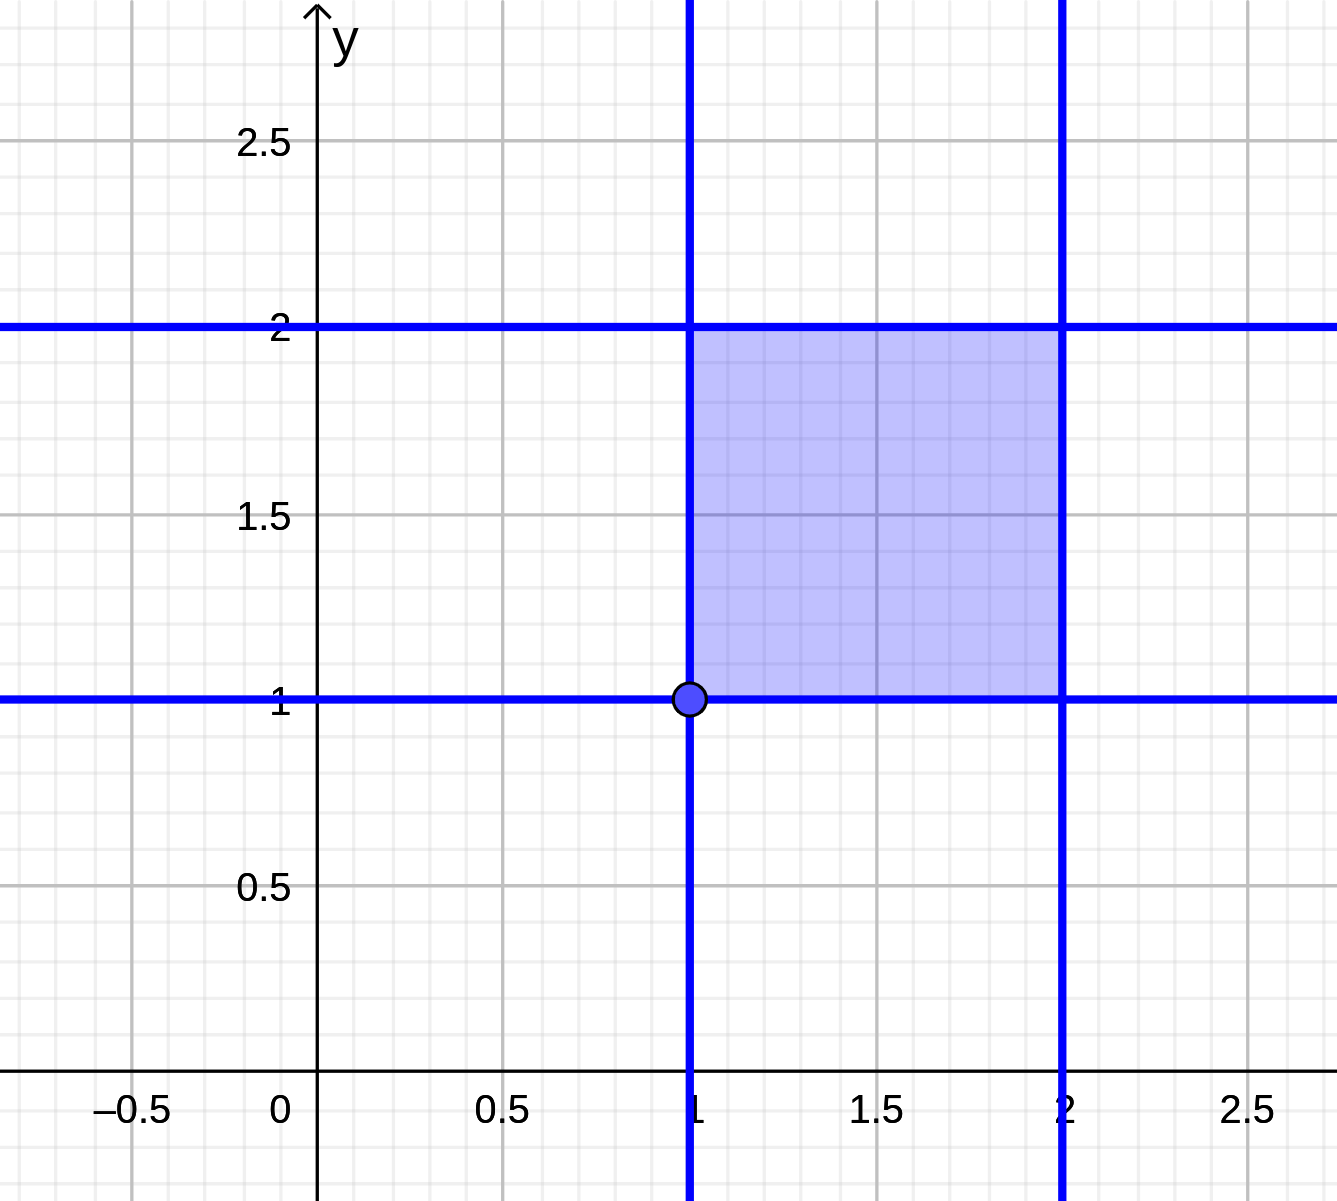
\includegraphics[scale=1.4]{img/ejercicios/1/12-b.png} 
\centering
\label{fig:1-12-b}
\end{figure}

La región definida por el cuadrado puede describirse entonces con dos simple inecuaciones:

\begin{equation}
\tcboxmath[colback=orange!25!white,colframe=orange,title=1.12.b]
{ \left\{ \begin{array}{ll}
1 \leq x \leq 2 \\
1 \leq y \leq 2
\end{array} \right. }
\end{equation}

\subsubsection*{1.12.c}
\label{subsubsec:1.12.c}
\addcontentsline{toc}{subsubsection}{\nameref{subsubsec:1.12.c}}

Directamente:

\begin{equation}
\tcboxmath[colback=orange!25!white,colframe=orange,title=1.12.c]
{ y > 2 x^2 }
\end{equation}

\subsubsection*{1.12.d}
\label{subsubsec:1.12.d}
\addcontentsline{toc}{subsubsection}{\nameref{subsubsec:1.12.d}}

Si los semiejes son $a=2$ y $b=4$, resulta:

\begin{equation}
\tcboxmath[colback=orange!25!white,colframe=orange,title=1.12.d]
{ \frac{x^2}{4} + \frac{y^2}{16} < 1 }
\end{equation}

\hrule
\vspace{10 pt}

\subsection*{1.13}
\label{subsec:1.13}
\addcontentsline{toc}{subsection}{\nameref{subsec:1.13}}

\textbf{Trazar aproximadamente las curvas descriptas (en coordenadas polares) por:}

\begin{enumerate}[(a)]
\bfseries
\item $\rho = 2, 0 \leq \phi \leq \pi/4$

\item $\phi = \pi/6, 1 \leq \rho \leq 2$

\item $\rho = \cos(\phi), 0 \leq \phi \leq \pi/2$
\end{enumerate}
\hrule

\subsubsection*{1.13.a}
\label{subsubsec:1.13.a}
\addcontentsline{toc}{subsubsection}{\nameref{subsubsec:1.13.a}}

El módulo está fijo, y varía el ángulo. Por lo tanto, esta curva es un arco sobre la circunferencia de radio 2 centrada en el origen. Va desde el ángulo cero a $\frac{\pi}{4} = 45^{\circ}$. Ver figura \ref{fig:1-13-a}.

\begin{figure}[ht]
\caption{\textbf{13-a}}
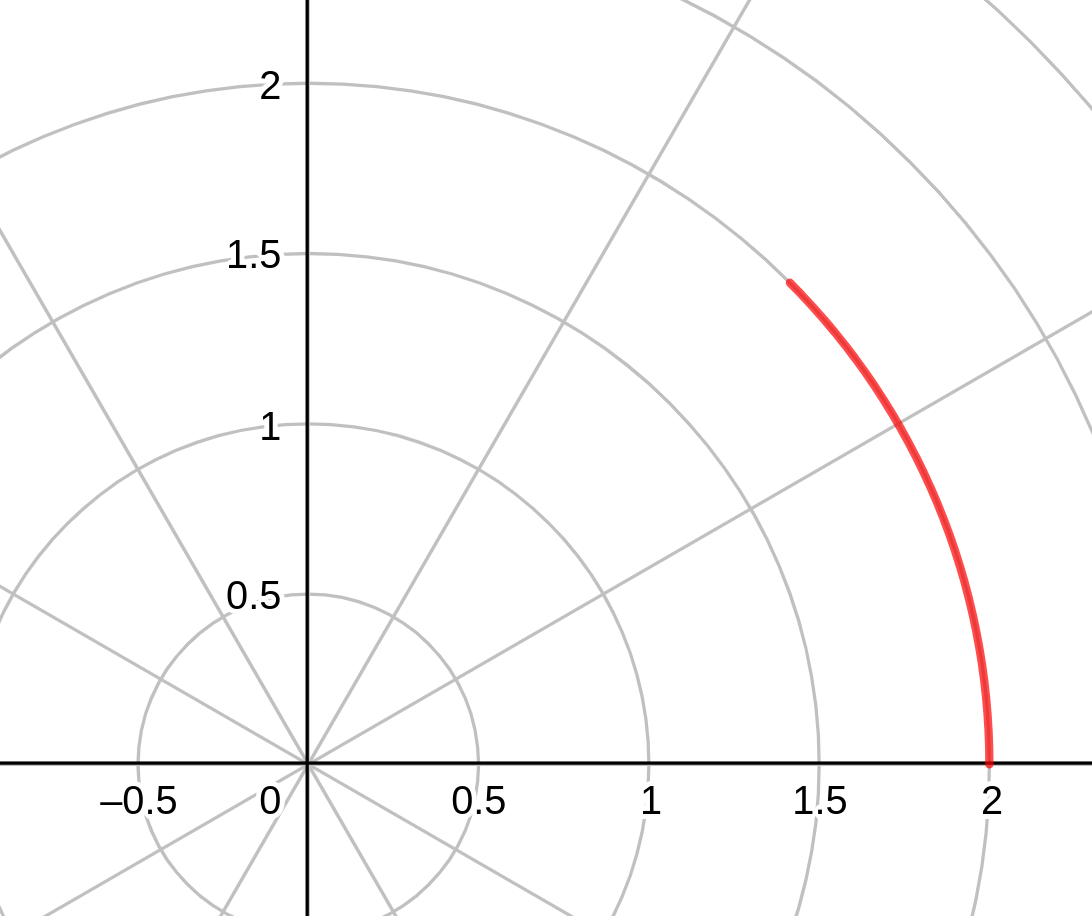
\includegraphics[scale=1.4]{img/ejercicios/1/13-a.png} 
\centering
\label{fig:1-13-a}
\end{figure}

\subsubsection*{1.13.b}
\label{subsubsec:1.13.b}
\addcontentsline{toc}{subsubsection}{\nameref{subsubsec:1.13.b}}

Ahora está fijo el ángulo, y varía el módulo. En este caso la curva será un segmento de la recta de pendiente $\frac{\pi}{6}= 30^{\circ}$ que pasa por el origen. Dicho segmento irá desde el punto que corta la circunferencia de radio 1 al punto que corta la circunferencia de radio 2. Ver figura \ref{fig:1-13-b}.

\begin{figure}[ht]
\caption{\textbf{13-b}}
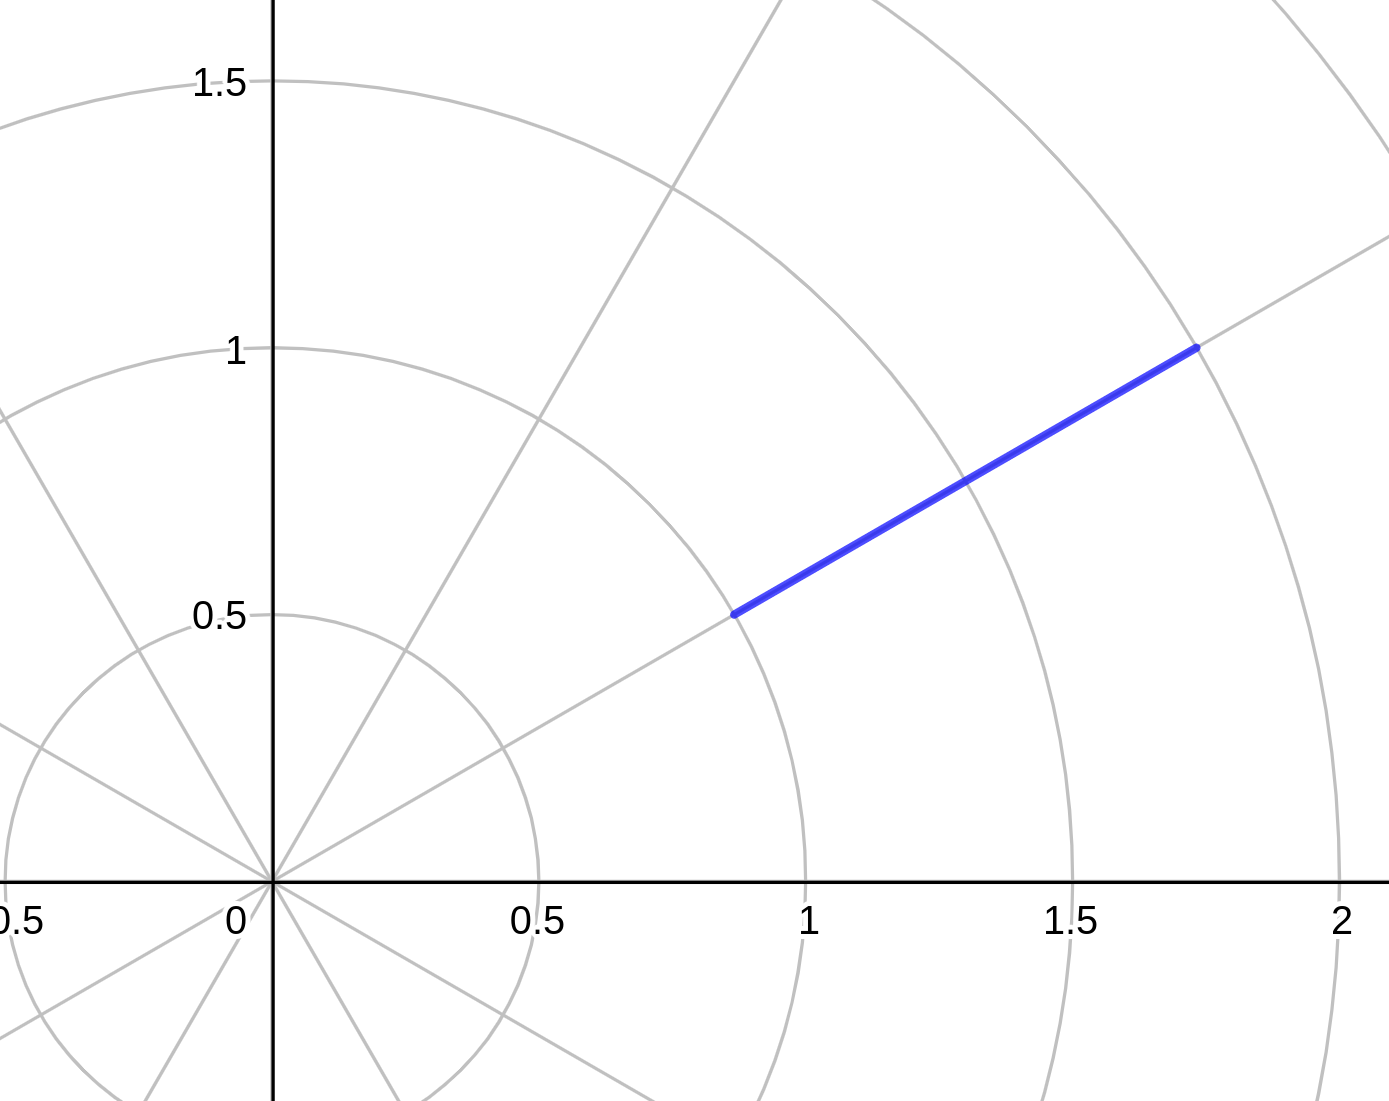
\includegraphics[scale=2.35]{img/ejercicios/1/13-b.png} 
\centering
\label{fig:1-13-b}
\end{figure}

\subsubsection*{1.13.c}
\label{subsubsec:1.13.c}
\addcontentsline{toc}{subsubsection}{\nameref{subsubsec:1.13.a}}

Esto no es tan directo de visualizar, por ello es útil hacer una tabla de valores.

\begin{center}
\begin{tabular}{ |c|c|c| }
 \hline
 $\phi$ (rad) & $\phi$ (deg) & $\rho$ \\ [0.5ex] 
 \hline\hline
 \hline
 0 & 0 & 1 \\ 
 $\pi/12$ & 15 & 0,96 \\ 
 $\pi/6$ & 30 & 0,86 \\
 $\pi/4$ & 45 & 0.71 \\
 $\pi/6$ & 60 & 0,86 \\
 $5\pi/12$ & 75 & 0,26 \\
 $\pi/2$ & 90 & 0 \\
 \hline
\end{tabular}
\end{center}

Graficando y uniendo los puntos, se obtiene la curva de la figura \ref{fig:1-13-c}.

\begin{figure}[ht]
\caption{\textbf{13-c}}
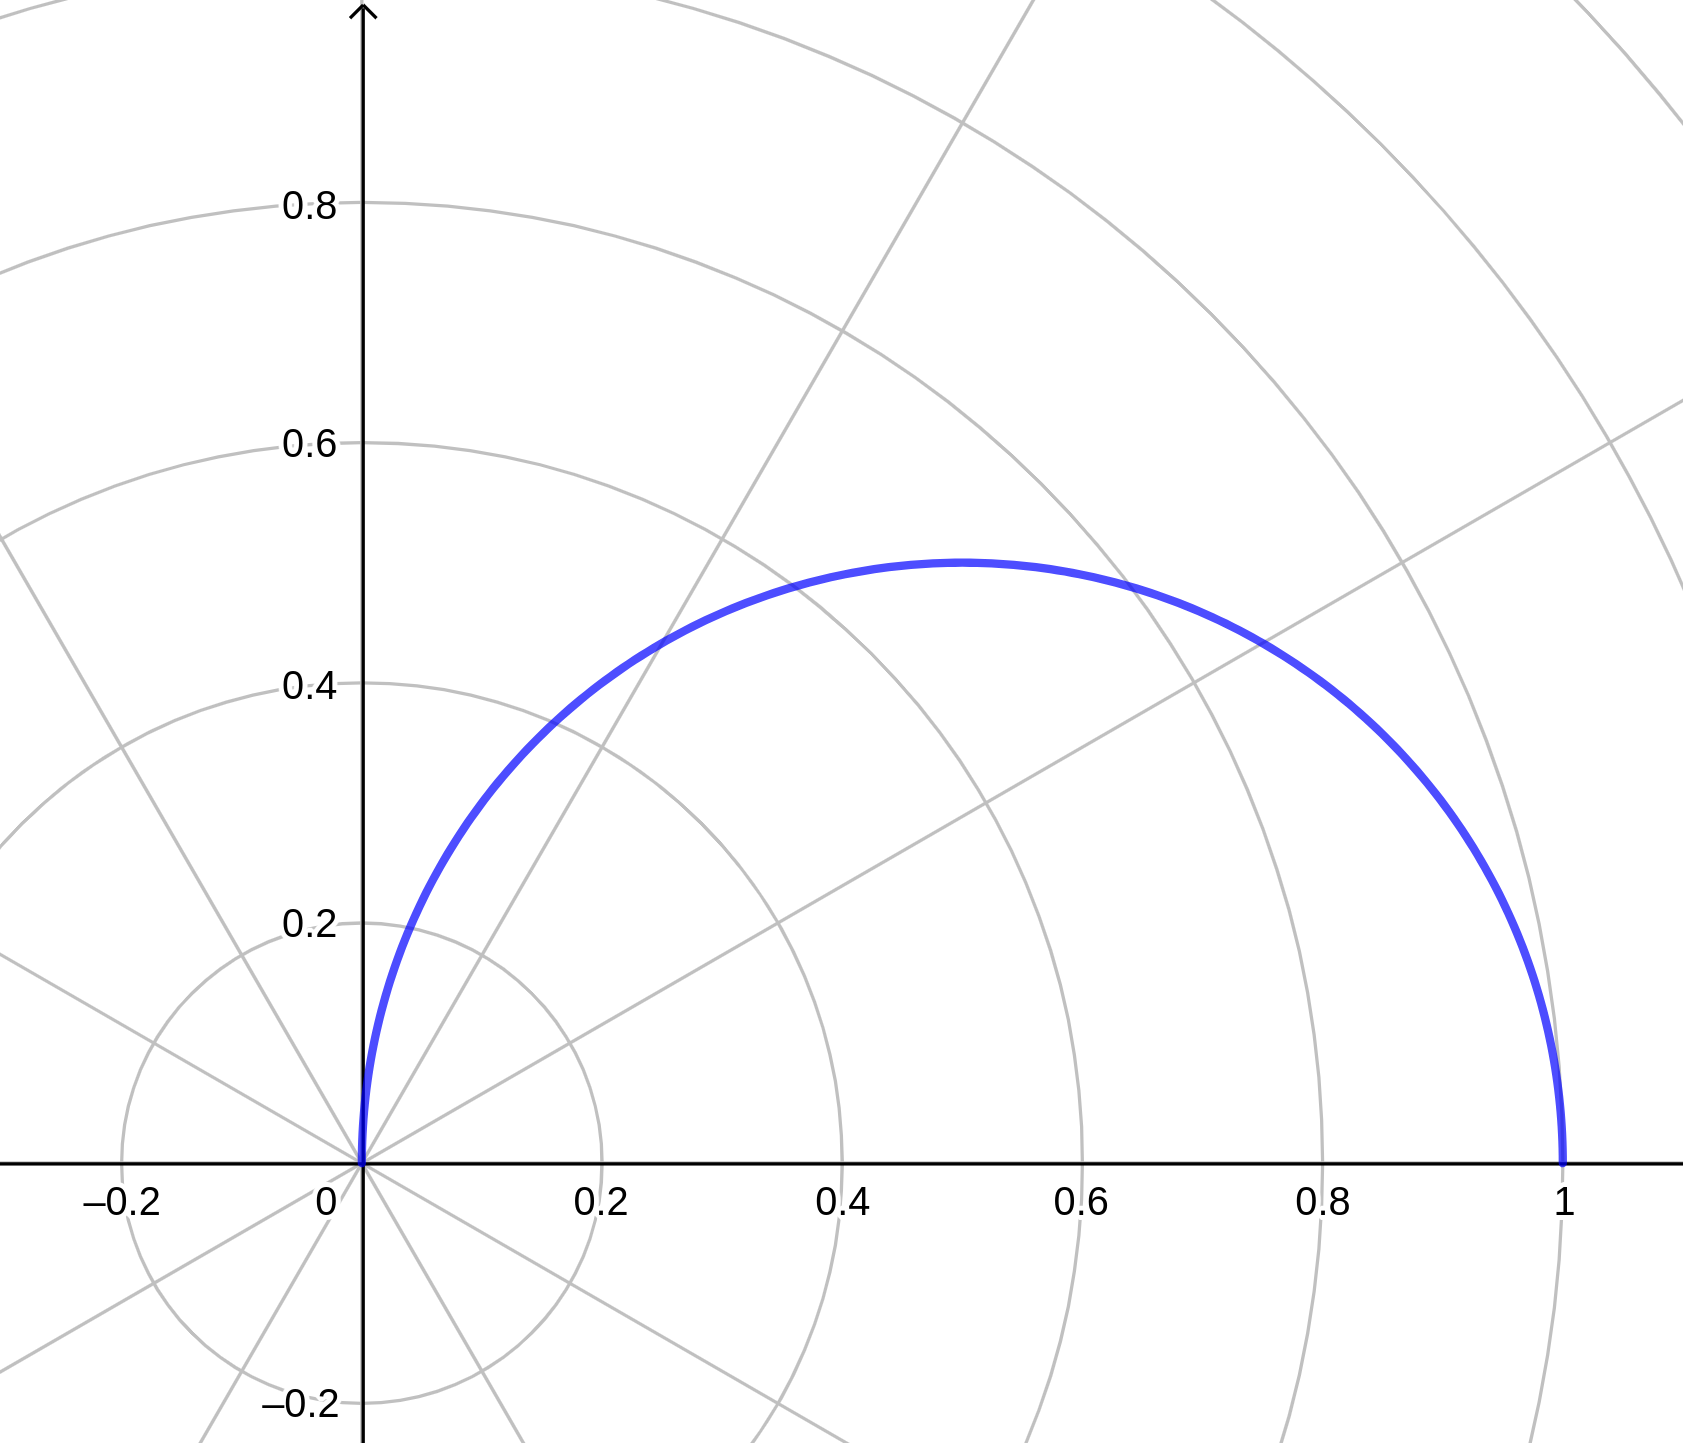
\includegraphics[scale=4.5]{img/ejercicios/1/13-c.png} 
\centering
\label{fig:1-13-c}
\end{figure}

Para intentar entender mejor este gráfico, es posible expresar la curva de forma paramétrica, recordando la equivalencia entre coordenadas cartesianas y polares.

\begin{equation}
(x, y) = (\rho \cos(\phi), \rho \sin(\phi))
\end{equation}

En este caso, el parámetro ideal es $\phi$, ya que $\rho$ depende de él. Renombrando $\phi$ a $t$, se obtiene:

\begin{equation}
(x(t), y(t)) = (\cos(t) \cos(t), \cos(t)\sin(t)) = (\cos^2(t), \cos(t) \sin(t))
\end{equation}

\hrule
\vspace{10 pt}

\subsection*{1.14}
\label{subsec:1.14}
\addcontentsline{toc}{subsection}{\nameref{subsec:1.14}}

\textbf{Describir mediante inecuaciones en coordenadas cartesianas las regiones planas descriptas (en coordenadas polares) por:}

\begin{enumerate}[(a)]
\bfseries
\item $\pi/6 \leq \phi \leq \pi/3$

\item $1 \leq \rho < 2$

\item $1 < \rho \leq 2, \pi/6 \leq \phi < \pi/3$

\item $\rho \geq \phi$
\end{enumerate}
\hrule

\subsubsection*{1.14.a}
\label{subsubsec:1.14.a}
\addcontentsline{toc}{subsubsection}{\nameref{subsubsec:1.14.a}}

Limitar el ángulo $\phi$ entre dos valores equivale a limitar las coordenadas cartesianas entre dos rectas que pasen por el origen y tengan pendiente dada por los ángulos.

\begin{subequations}
\begin{align}
& m_1 = \arctan(\pi/6) \approx 0,4823 \\
& m_2 = \arctan(\pi/3) \approx 0,8084
\end{align}
\end{subequations}

\begin{equation}
\tcboxmath[colback=orange!25!white,colframe=orange,title=1.14.a]
{ m_1 x \leq y \leq m_2 x }
\end{equation}

\subsubsection*{1.14.b}
\label{subsubsec:1.14.b}
\addcontentsline{toc}{subsubsection}{\nameref{subsubsec:1.14.b}}

Análogamente al inciso anterior, esta región es la abarcada entre dos círculos.

\begin{equation}
\tcboxmath[colback=orange!25!white,colframe=orange,title=1.14.b]
{ 1^2 \leq x^2 + y^2 < 2^2 }
\end{equation}

\subsubsection*{1.14.c}
\label{subsubsec:1.14.c}
\addcontentsline{toc}{subsubsection}{\nameref{subsubsec:1.14.c}}

Es la intersección entre (a) y (b), teniendo en cuenta que cambian los extremos.

\begin{equation}
\tcboxmath[colback=orange!25!white,colframe=orange,title=1.14.c]
{ \left\{ \begin{array}{ll}
m_1 x \leq y < m_2 x \\
1^2 < x^2 + y^2 \leq 2^2
\end{array} \right. }
\end{equation}

\subsubsection*{1.14.d}
\label{subsubsec:1.14.d}
\addcontentsline{toc}{subsubsection}{\nameref{subsubsec:1.14.d}}

Si el módulo es mayor o igual al argumento, claramente esta región incluye $x^2 + y^2 >= (2\pi)^2$. En el interior de esa circunferencia, la forma más directa es transformar las coordenadas.

\begin{subequations}
\begin{align}
& \rho = \sqrt{x^2 + y^2} \\
& \phi = \arctan(y/x)
\end{align}
\end{subequations}

De forma general, resulta entonces:

\begin{equation}
\tcboxmath[colback=orange!25!white,colframe=orange,title=1.14.d]
{ \sqrt{x^2 + y^2} \geq \arctan \left( \frac{y}{x} \right) }
\end{equation}

\hrule
\vspace{10 pt}

\subsection*{1.15}
\label{subsec:1.15}
\addcontentsline{toc}{subsection}{\nameref{subsec:1.15}}

\textbf{Describir mediante inecuaciones en coordenadas polares las regiones planas descriptas (en coordenadas cartesianas) por:}

\begin{enumerate}[(a)]
\bfseries
\item $x^2 + y^2 \leq 1$

\item $x^2 + y^2 - 2y \leq 0, y > |x|$

\item $x^2 \geq 3y^2$

\item $x \geq y, x < 3y$
\end{enumerate}
\hrule

\subsubsection*{1.15.a}
\label{subsubsec:1.15.a}
\addcontentsline{toc}{subsubsection}{\nameref{subsubsec:1.15.a}}

Es el interior de un círculo de radio 1, ergo:

\begin{equation}
\tcboxmath[colback=orange!25!white,colframe=orange,title=1.15.a]
{ A = \{ (\rho, \phi) \in \Bbb R^2 / \rho \leq 1 \} }
\end{equation}

\subsubsection*{1.15.b}
\label{subsubsec:1.15.b}
\addcontentsline{toc}{subsubsection}{\nameref{subsubsec:1.15.b}}

De las dos restricciones, $y > |x|$ se traduce directamente a polares.

\begin{figure}[ht]
\caption{\textbf{15-b}}
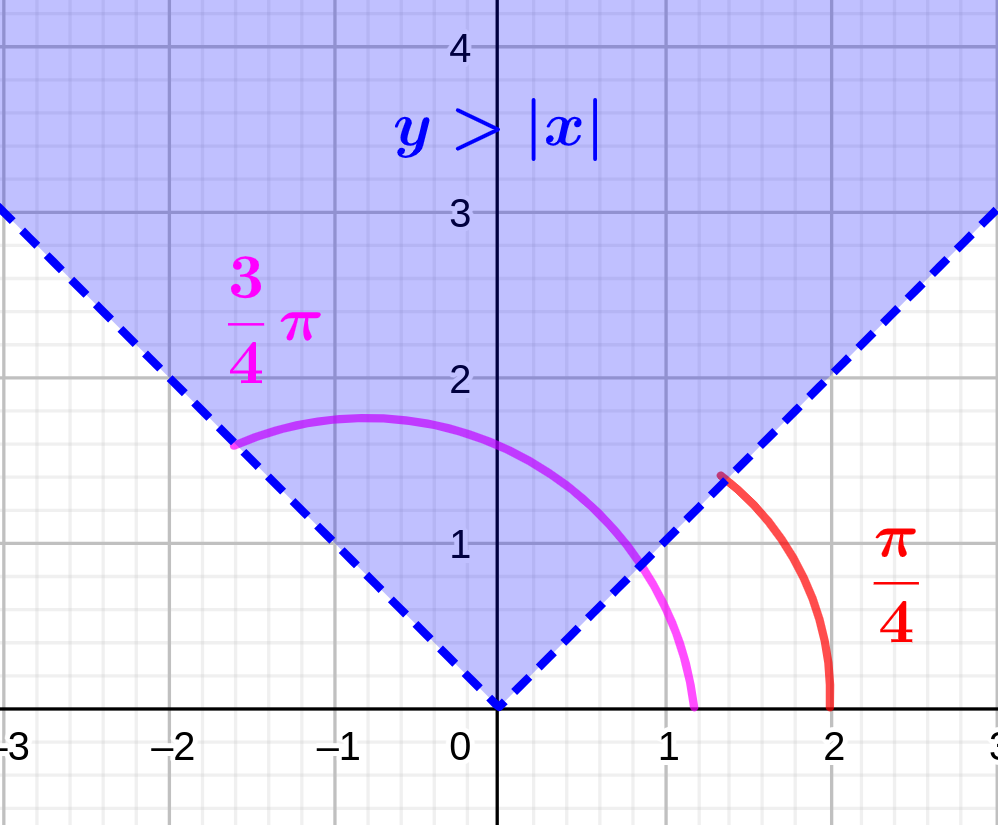
\includegraphics[scale=1]{img/ejercicios/1/15-b.png} 
\centering
\label{fig:1-15-b}
\end{figure}

Así, $y > |x|$ en polares es $pi/4 < \phi < 3\pi/4$. Para la otra restricción, se puede reescribir utilizando las igualdades:

\begin{subequations}
\begin{align}
& x^2 + y^2 = \rho^2 \\
& x = \rho \cos(\phi) \\
& y = \rho \sin(\phi)
\end{align}
\end{subequations}

Resulta entonces:

\begin{equation}
\rho^2 - 2 \sin(\phi) \leq 0 \Rightarrow \rho (\rho - 2 \sin(\phi)) \leq 0 \Rightarrow \rho \leq 2 \sin(\phi)
\end{equation}

En el paso en que se divide por $\rho$ miembro a miembro, se asume $\rho$ distinto de cero. La desigualdad resultante sigue satisfaciéndose para $\rho = 0, \phi = 0$, así que no hay problema.

\begin{equation}
\tcboxmath[colback=orange!25!white,colframe=orange,title=1.15.b]
{ \left\{ \begin{array}{ll}
\rho \leq 2 \sin(\phi) \\
\frac{\pi}{4} < \phi < \frac{3}{4} \pi
\end{array} \right. }
\end{equation}

\subsubsection*{1.15.c}
\label{subsubsec:1.15.c}
\addcontentsline{toc}{subsubsection}{\nameref{subsubsec:1.15.c}}

Tomando raíz cuadrada miembro a miembro, resulta:

\begin{equation}
|x| \geq \sqrt{3} |y|
\end{equation}

Para $y > 0$, resulta:

\begin{equation}
y \leq \frac{1}{\sqrt{3}} |x|
\end{equation}

Y para $y < 0$:

\begin{equation}
y \geq -\frac{1}{\sqrt{3}} |x|
\end{equation}

Gráficamente:

\begin{figure}[ht]
\caption{\textbf{15-c}}
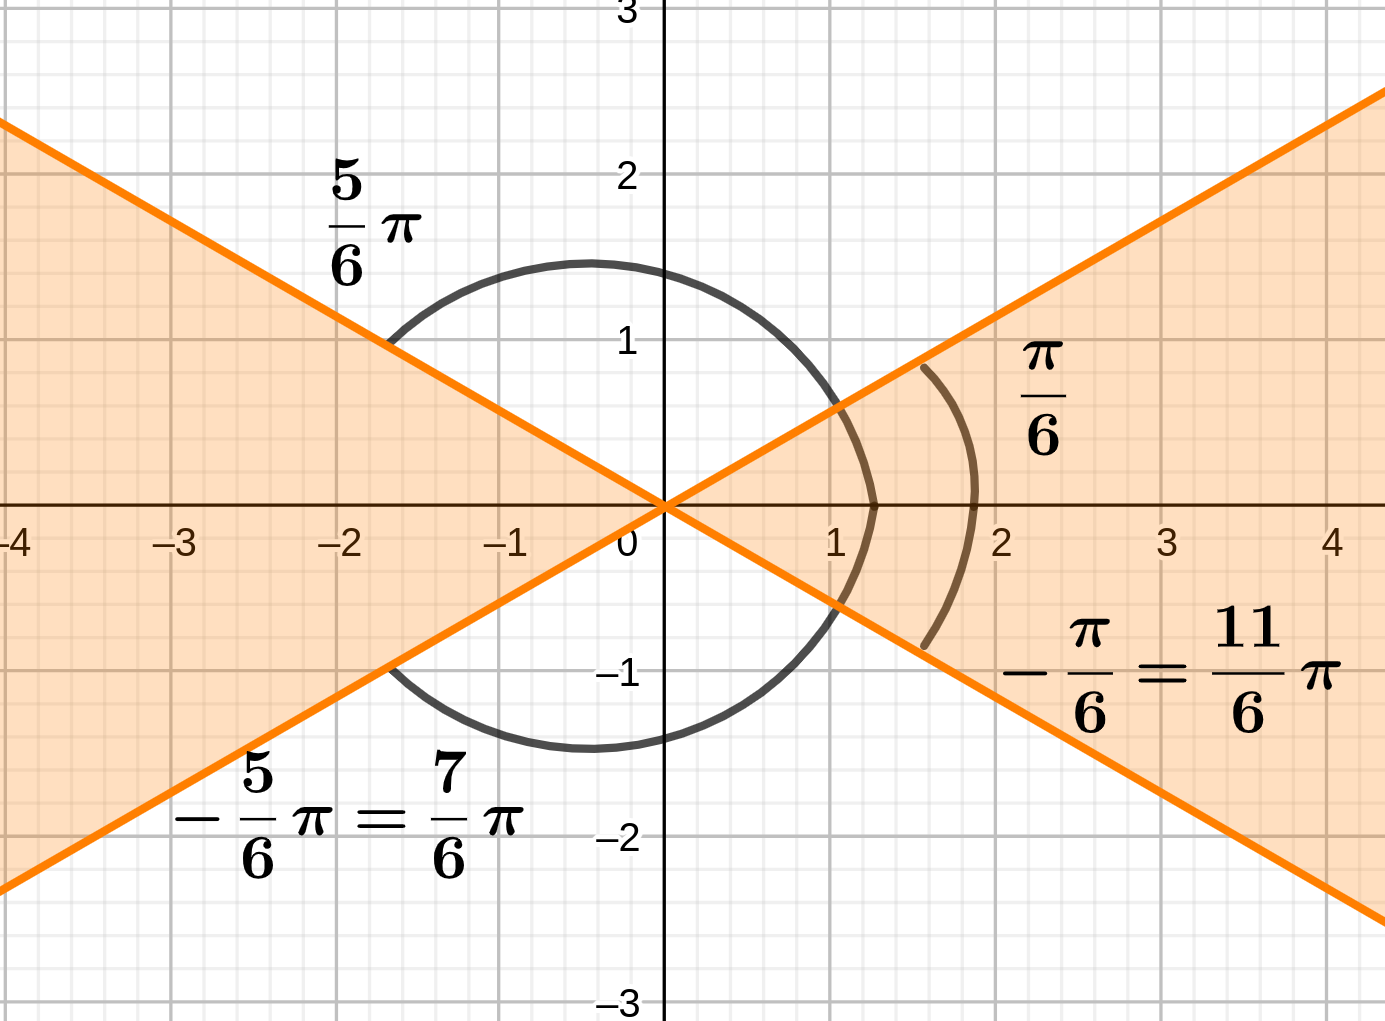
\includegraphics[scale=1]{img/ejercicios/1/15-c.png} 
\centering
\label{fig:1-15-c}
\end{figure}

Finalmente:

\begin{equation}
\tcboxmath[colback=orange!25!white,colframe=orange,title=1.15.c]
{ \left\{ \begin{array}{ll}
-\frac{\pi}{6} \leq \phi \leq \frac{\pi}{6} \\
\frac{5}{6}\pi \leq \phi \leq \frac{7}{6}\pi
\end{array} \right. }
\end{equation}

\subsubsection*{1.15.d}
\label{subsubsec:1.15.d}
\addcontentsline{toc}{subsubsection}{\nameref{subsubsec:1.15.d}}

Es el área entre dos rectas; puede expresarse en polares acotando el ángulo entre las dos pendientes.

\begin{equation}
\left\{
\begin{array}{ll}
x \geq y \\
x < 3y
\end{array}
\right. \Rightarrow \left\{
\begin{array}{ll}
y \leq x \\
y > \frac{1}{3} x
\end{array}
\right.
\end{equation}

En polares:

\begin{equation}
\arctan \left( \frac{1}{3} \right) < \phi < \frac{\pi}{4}
\end{equation}

\begin{equation}
\tcboxmath[colback=orange!25!white,colframe=orange,title=1.15.d]
{ 0,3218 < \phi < \frac{\pi}{4} }
\end{equation}

\hrule
\vspace{10 pt}

\subsection*{1.16}
\label{subsec:1.16}
\addcontentsline{toc}{subsection}{\nameref{subsec:1.16}}

\textbf{Describir mediante inecuaciones el interior y frontera de los conjuntos dados por:}

\begin{enumerate}[(a)]
\bfseries
\item $0 < x^2 + y^2 < 1$ (en $\Bbb R^2$)

\item $0 < x^2 + y^2 < 1$ (en $\Bbb R^3$)

\item $x \geq 0, y < 0$ (en $\Bbb R^2$)

\item $x^2 + y^2 \leq 1$ (en $\Bbb R^2$)

\item $x + y = 1$ (en $\Bbb R^2$)

\item $0 < |x| + |y| \leq 1$ (en $\Bbb R^2$)

\item $x \leq 0, y > 1, z<2$ (en $\Bbb R^3$)

\item $x^2 + y^2 <1, y + z > 2$ (en $\Bbb R^3$)

\item $0 < (x-z)^2 + (y-z)^2 < 1$ (en $\Bbb R^3$)

\item $1 \leq x^2 + y^2 + z^2 \leq 5$ (en $\Bbb R^3$)
\end{enumerate}
\hrule

\subsubsection*{1.16.a}
\label{subsubsec:1.16.a}
\addcontentsline{toc}{subsubsection}{\nameref{subsubsec:1.16.a}}

Gráficamente, esta región es el interior del círculo de radio 1 centrado en el origen, excluyendo al origen. Ver figura \ref{fig:1-16-a}.

\begin{figure}[ht]
\caption{\textbf{16-a}}
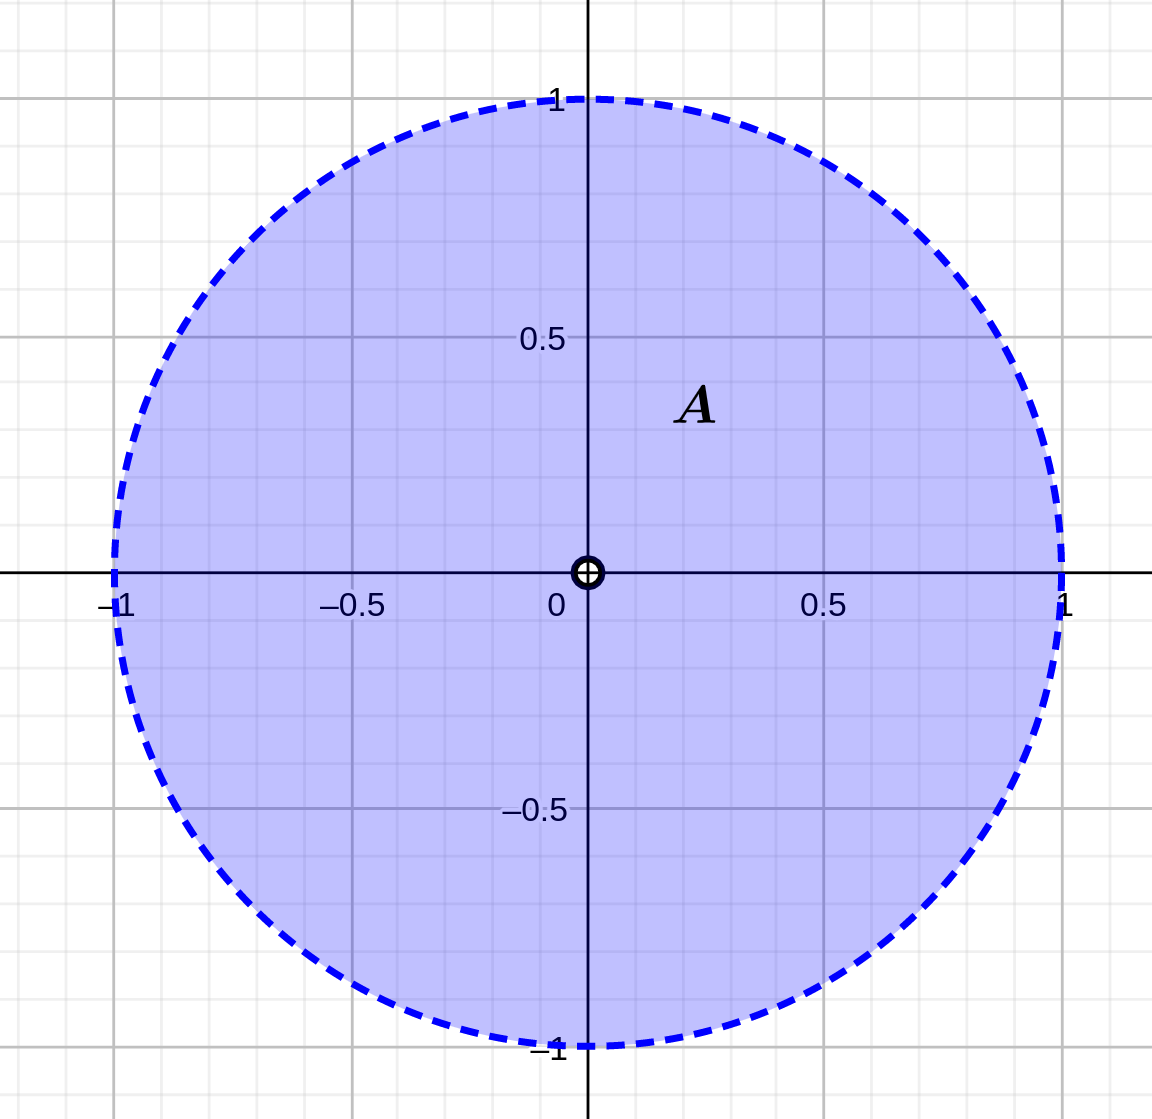
\includegraphics[scale=2.5]{img/ejercicios/1/16-a.png} 
\centering
\label{fig:1-16-a}
\end{figure}

Utilizando la notación de la teórica, el conjunto $A$ a analizar es:

\begin{equation}
A = \{ (x,y) \in \Bbb R^2 / 0 < x^2 + y^2 < 1 \}
\end{equation}

Para cualquier conjunto $A \in \Bbb R^n$, un punto $P_0$ es interior si existe al menos un entorno centrado en $P_0$ incluido completamente en $A$. El conjunto de puntos interiores de $A$ se denomina el interior de A, y se denota con el símbolo $A^{\circ}$. En este caso en particular, estando en $\Bbb R^2$, los entornos son círculos y se observa gráficamente que $A = A^{\circ}$: todo punto de A puede rodearse con un círculo completamente contenido en $A$, haciendo el radio tan chico como sea necesario.

\begin{equation}
\tcboxmath[colback=orange!25!white,colframe=orange, title=1.16.a) Conjunto interior]
{ A^{\circ} = A = \{ (x,y) \in \Bbb R^2 / 0 < x^2 + y^2 < 1 \}  }
\end{equation}

En cuanto a la frontera, la misma está constituida, por definición, por los puntos tales que todo entorno centrado en ellos contiene puntos tanto de $A$ como de $A^C$ (el complemento de A). En este caso, ese conjunto está formado por la circunferencia de radio 1, y el origen. Cualquier círculo centrado en un punto sobre la circunferencia contiene un punto que no pertenece a $A$: el centro del círculo, porque la circunferencia de radio 1 está excluida de $A$ por ser la desigualdad estricta. Y ese entorno también contendrá puntos de $A$, porque en tanto el radio sea mayor a cero, tomará algunos puntos del interior. Lo mismo ocurre con el origen.

\begin{equation}
\tcboxmath[colback=orange!25!white,colframe=orange, title=1.16-a) Conjunto frontera]
{ \partial{A} = (0,0) \cup \{ (x,y) \in \Bbb R^2 / x^2 + y^2 = 1 \}  }
\end{equation}

\subsubsection*{1.16.b}
\label{subsubsec:1.16.b}
\addcontentsline{toc}{subsubsection}{\nameref{subsubsec:1.16.b}}

La misma desigualdad del inciso anterior, pero en $\Bbb R^3$, pasa a ser el interior del cilindro de radio 1 centrado en el origen, excluyendo al eje $z$ (a lo largo del cual $x = 0 \wedge y = 0$ y no se cumple la desigualdad). Como ocurría en el caso anterior, las desigualdades estrictas hacen que este sea un conjunto abierto. El análisis en base a entornos ahora se hace con esferas. Cualquier esfera centrada en un punto dentro del cilindro puede reducir su radio de manera tal que todos los puntos de la esfera estén contenidos en $A$. Ergo:

\begin{equation}
\tcboxmath[colback=orange!25!white,colframe=orange, title=1.16.b) Conjunto interior]
{ A^{\circ} = A = \{ (x, y, z) \in \Bbb R^3 / 0 < x^2 + y^2 < 1 \}  }
\end{equation}

Y análogamente, toda esfera centrada en la cara externa del cilindro, o en el eje $z$, contendrá tanto puntos de $A$ como de $A^C$. Por lo tanto:

\begin{equation}
\tcboxmath[colback=orange!25!white,colframe=orange, title=1.16.b) Conjunto frontera]
{ \partial{A} = \{(x, y, z) \in \Bbb R^3 / x = 0 \wedge y = 0 \} \cup \{ (x, y, z) \in \Bbb R^3 / x^2 + y^2 = 1 \}  }
\end{equation}

\subsubsection*{1.16.c}
\label{subsubsec:1.16.c}
\addcontentsline{toc}{subsubsection}{\nameref{subsubsec:1.16.c}}

El conjunto $A$ en este caso es:

\begin{equation}
A = \{ (x,y) \in \Bbb R^2 / x \geq 0 \wedge y < 0 \}
\end{equation}

Gráficamente, los puntos de $A$ son los de la figura \ref{fig:1-16-c}.

\begin{figure}[ht]
\caption{\textbf{16-c}}
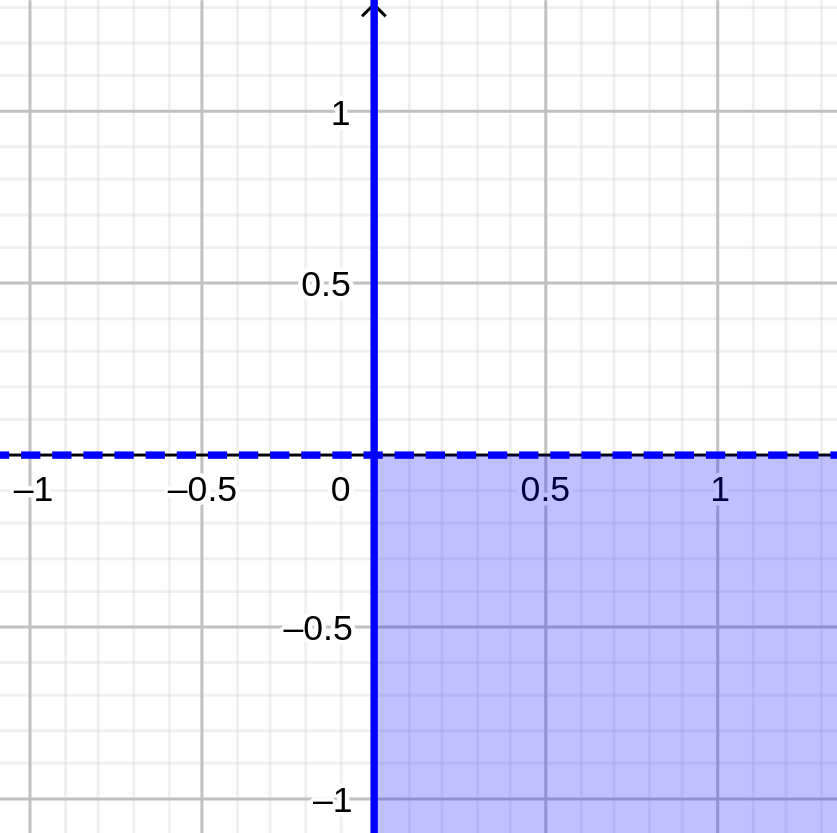
\includegraphics[scale=2.5]{img/ejercicios/1/16-c.png} 
\centering
\label{fig:1-16-c}
\end{figure}

El conjunto $A$ es entonces el cuarto cuadrante del plano $xy$, pero excluyendo el semieje $x$ positivo y el origen. Por lo tanto, su interior se obtiene quitándole el semieje negativo $y$. Si se tomara un punto de dicho semieje, para cualquier radio positivo, el entorno contendría puntos externos. En consecuencia:

\begin{equation}
\tcboxmath[colback=orange!25!white,colframe=orange, title=1.16.c) Conjunto interior]
{ A^{\circ} = \{ (x, y) \in \Bbb R^2 / x > 0 \wedge y < 0 \}  }
\end{equation}

En cuanto a la frontera, está formada por el semieje positivo $x$, y el semieje negativo $y$. Cualquier entorno centrado en un punto de ambos contendrá puntos de $A$ y $A^C$. El origen también es punto frontera.

\begin{equation}
\tcboxmath[colback=orange!25!white,colframe=orange, title=1.16.c) Conjunto frontera]
{ \partial{A} = (0,0) \cup \{ (x, y) \in \Bbb R^2 / x = 0 \wedge y < 0 \} \cup \{ (x, y) \in \Bbb R^2 / y = 0 \wedge x > 0 \} }
\end{equation}

\subsubsection*{1.16.d}
\label{subsubsec:1.16.d}
\addcontentsline{toc}{subsubsection}{\nameref{subsubsec:1.16.d}}

El conjunto $A$ es en este caso:

\begin{equation}
A = \{ (x,y) \in \Bbb R^2 / x^2 + y^2 \leq 1 \}
\end{equation}

Gráficamente, los puntos de $A$ son los indicados en la figura \ref{fig:1-16-d}.

\begin{figure}[ht]
\caption{\textbf{16-d}}
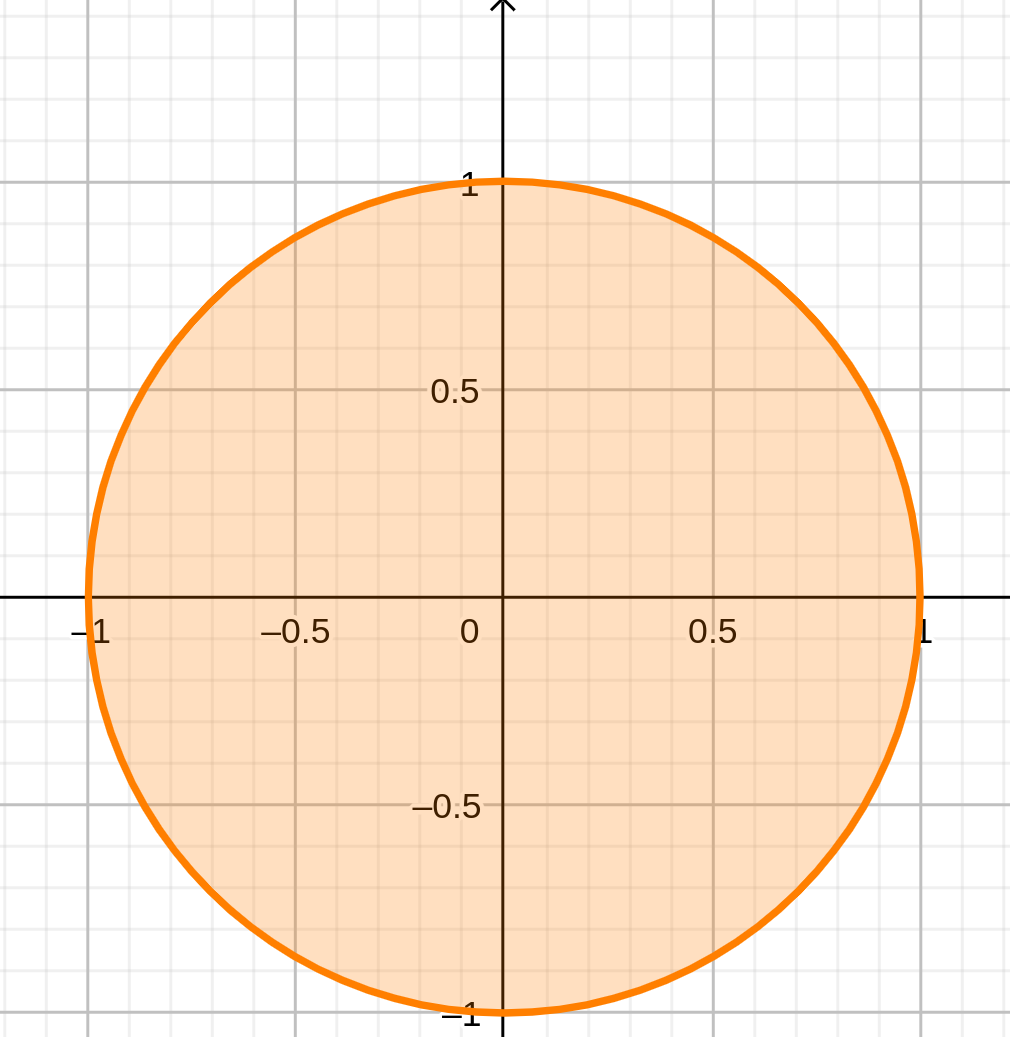
\includegraphics[scale=2.5]{img/ejercicios/1/16-d.png} 
\centering
\label{fig:1-16-d}
\end{figure}

Resulta directo entonces, con los criterios utilizados en los incisos previos, que:

\begin{equation}
\tcboxmath[colback=orange!25!white,colframe=orange, title=1.16.d) Conjunto interior]
{ A^{\circ} = \{ (x, y) \in \Bbb R^2 / x^2 + y^2 < 1 \}  }
\end{equation}

\begin{equation}
\tcboxmath[colback=orange!25!white,colframe=orange, title=1.16.d) Conjunto frontera]
{ \partial{A} = \{ (x, y) \in \Bbb R^2 / x^2 + y^2 = 1 \} }
\end{equation}

\subsubsection*{1.16.e}
\label{subsubsec:1.16.e}
\addcontentsline{toc}{subsubsection}{\nameref{subsubsec:1.16.e}}

El conjunto $A$ puede definirse como:

\begin{equation}
A = \{ (x, y) \in \Bbb R^2 / x + y = 1 \}
\end{equation}

No es necesario graficar los puntos del conjunto para determinar que corresponden a la recta $y = -x + 1$. En el caso de una recta, cualquier punto de la misma que se tome tendrá puntos de $A$ y puntos de $A^C$ en todos sus entornos. Por lo tanto, el interior de $A$ es el conjunto vacío, y su frontera es el mismo conjunto $A$.

\begin{equation}
\tcboxmath[colback=orange!25!white,colframe=orange,title=1.16.e]
{ A^{\circ} = \emptyset }
\end{equation}

\begin{equation}
\tcboxmath[colback=orange!25!white,colframe=orange,title=1.16.e) Conjunto frontera]
{ \partial{A} = A = \{ (x, y) \in \Bbb R^2 / x + y = 1 \} }
\end{equation}

\subsubsection*{1.16.f}
\label{subsubsec:1.16.f}
\addcontentsline{toc}{subsubsection}{\nameref{subsubsec:1.16.f}}

En primer lugar, será de utilidad graficar el conjunto $A = \{ (x,y) \in \Bbb R^2 / 0 < |x| + |y| \leq 1 \}$. Dicho conjunto puede pensarse como la intersección de dos regiones:

\begin{equation}
\left\{
\begin{array}{ll}
0 < |x| + |y| \\
|x| + |y| \leq 1
\end{array}
\right. \Rightarrow
\left\{
\begin{array}{ll}
-|x| < |y| \\
|y| \leq -|x| + 1
\end{array}
\right.
\end{equation}

Para el caso $y \geq 0$, resulta:$|y| = y$:

\begin{equation}
\left\{
\begin{array}{ll}
-|x| < y \\
y \leq -|x| + 1
\end{array}
\right.
\end{equation}

Para el caso $y < 0$:

\begin{equation}
\left\{
\begin{array}{ll}
-|x| < -y \\
-y \leq -|x| + 1
\end{array}
\right. \Rightarrow
\left\{
\begin{array}{ll}
y > |x| \\
y \geq |x| - 1
\end{array}
\right.
\end{equation}

\begin{figure}[ht]
\caption{\textbf{16-f}}
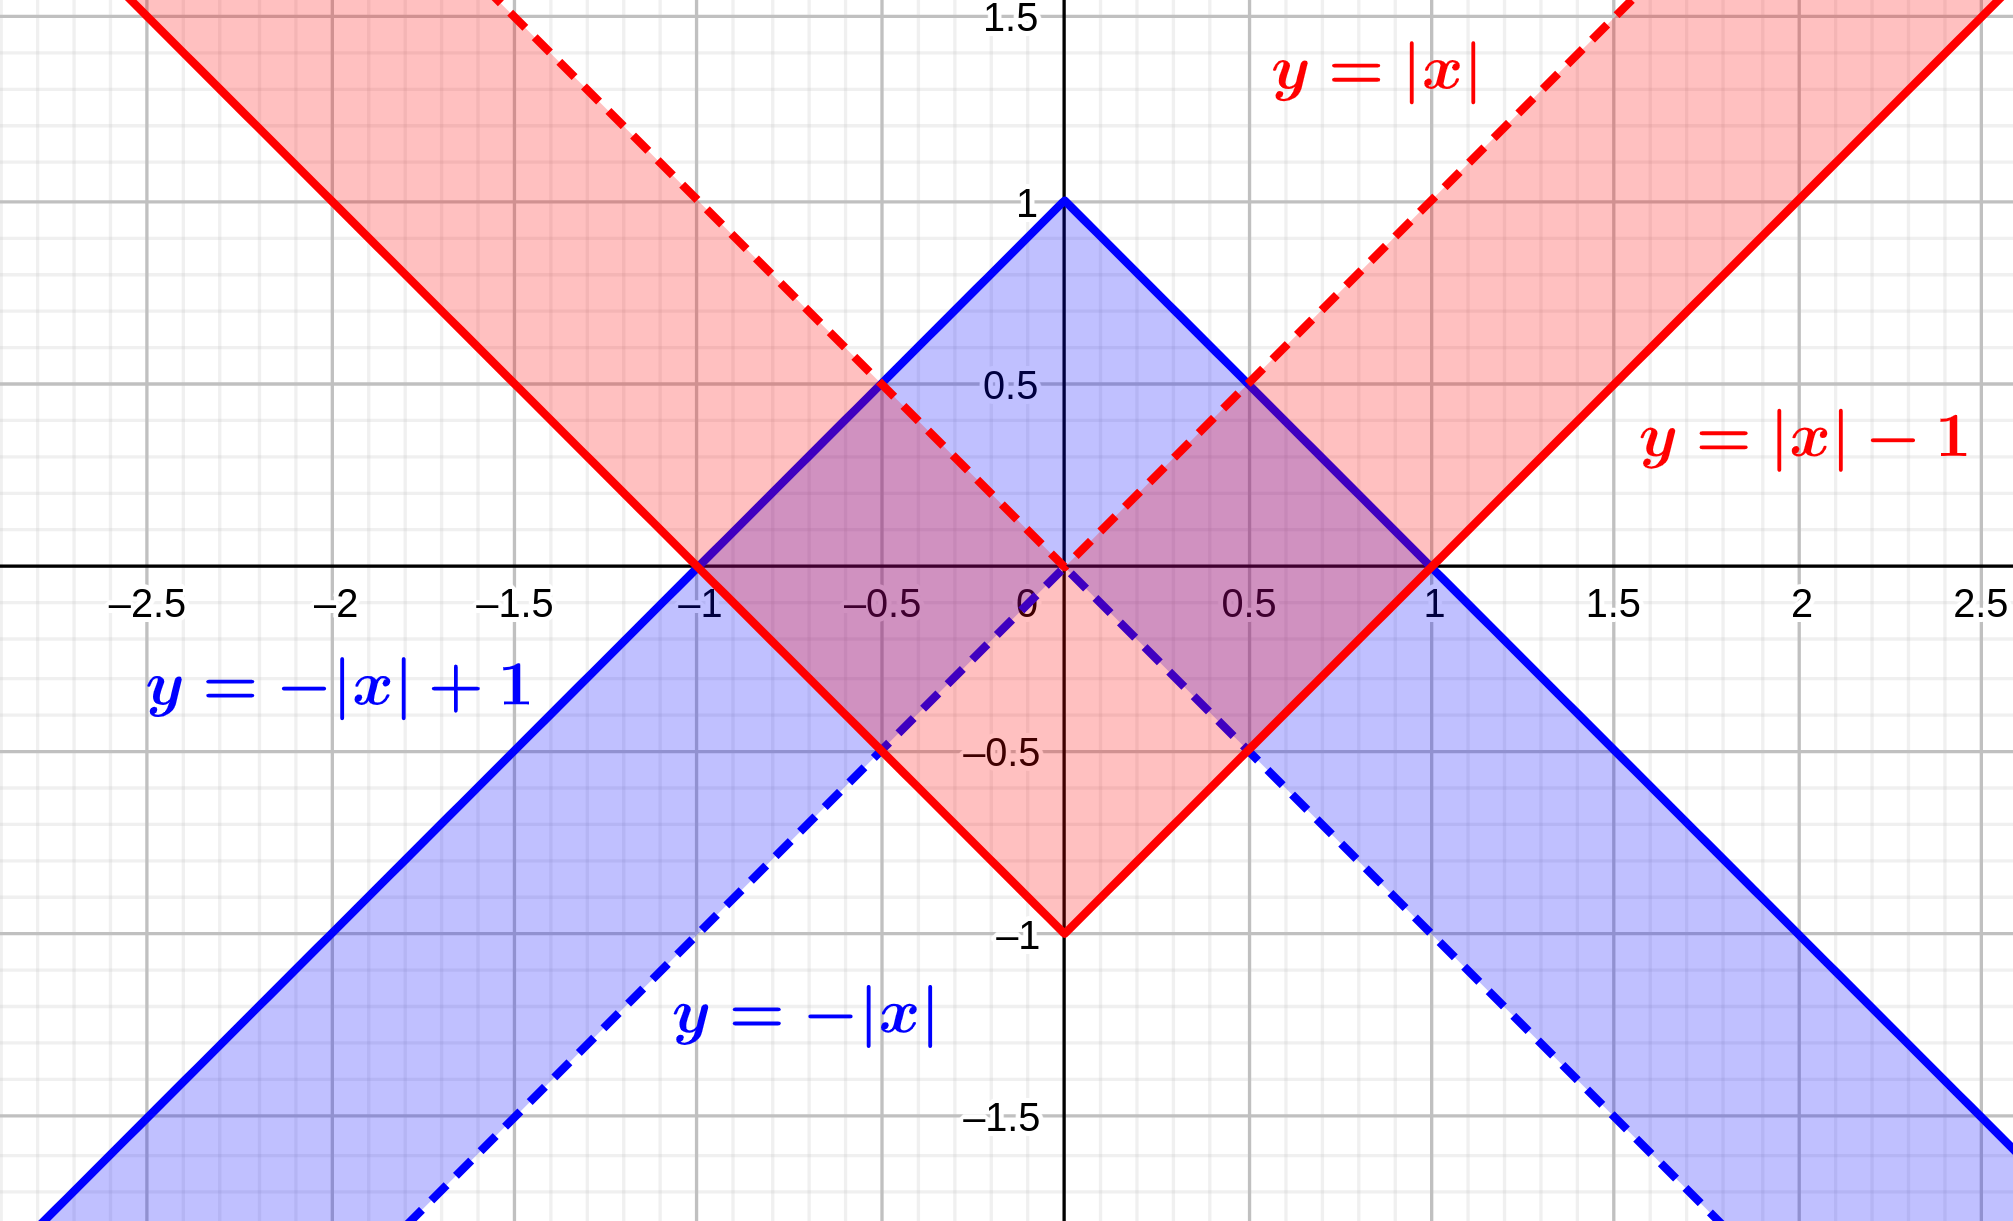
\includegraphics[scale=2.5]{img/ejercicios/1/16-f.png} 
\centering
\label{fig:1-16-f}
\end{figure}

En la figura \ref{fig:1-16-f}, se puede ver en azul el caso $y \geq 0$, y en rojo $y < 0$. La intersección de ambos es el conjunto $A$. El interior de $A$, entonces, se obtiene cambiando la desigualdad con 1 por una desigualdad estricta:

\begin{equation}
\tcboxmath[colback=orange!25!white,colframe=orange,title=1.16.f) Interior]
{ A^{\circ} = \{ (x,y) \in \Bbb R^2 / 0 < |x| + |y| < 1 \} }
\end{equation}

Para la frontera, se puede definir tomando secciones de las funciones que la delimitan. Observando de nuevo la figura \ref{fig:1-16-f}, donde están rotuladas dichas funciones, resulta:

\begin{equation}
\tcboxmath[colback=orange!25!white,colframe=orange,title=1.16.f) Frontera]
{ 
\begin{array}{ll}
\partial{A} = & \left\{ (x,y) \in \Bbb R^2 / y = -|x|+1, -1 \leq x \leq -\frac{1}{2} \right\} \\
& \cup \left\{ (x,y) \in \Bbb R^2 / y = |x|, -\frac{1}{2} \leq x \leq \frac{1}{2} \right\} \\
& \cup \left\{ (x,y) \in \Bbb R^2 / y = -|x|+1, \frac{1}{2} \leq x \leq 1 \right\} \\
& \cup \left\{ (x,y) \in \Bbb R^2 / y = |x|-1, -1 \leq x \leq -\frac{1}{2} \right\} \\
& \cup \left\{ (x,y) \in \Bbb R^2 / y = -|x|, -\frac{1}{2} \leq x \leq \frac{1}{2} \right\} \\
& \cup \left\{ (x,y) \in \Bbb R^2 / y = |x|-1, \frac{1}{2} \leq x \leq 1 \right\} \\
\end{array}
}
\end{equation}

\subsubsection*{1.16.g}
\label{subsubsec:1.16.g}
\addcontentsline{toc}{subsubsection}{\nameref{subsubsec:1.16.g}}

Para visualizar $A$, una forma es visualizarlo en el plano $(x, y)$ y extenderlo a 3 dimensiones. Considerando sólo $x$ e $y$, se tiene el semiplano de la figura \ref{fig:1-16-g}. 

\begin{figure}[ht]
\caption{\textbf{16-g}}
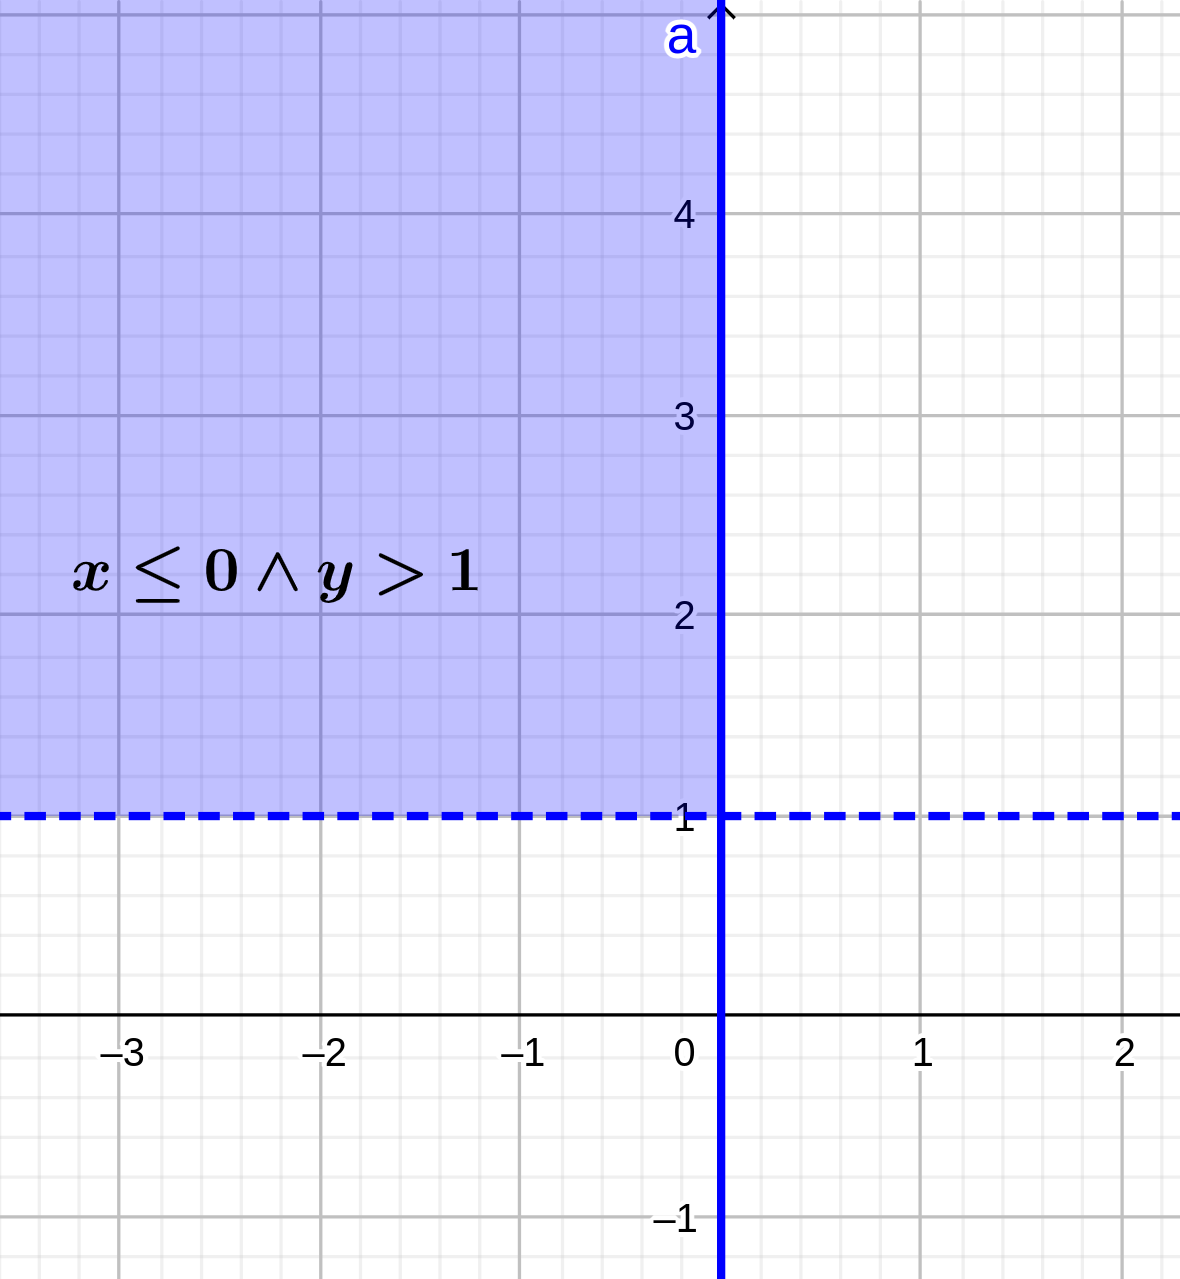
\includegraphics[scale=1]{img/ejercicios/1/16-g.png} 
\centering
\label{fig:1-16-g}
\end{figure}

Para extender esto a 3 dimensiones, alcanza con imaginar que el gráfico del plano $(x,y)$ corresponde a $z = 0$, y se repite para todo $z < 2$. O sea que $A$ es una región infinita delimitada por tres planos. Tiene un vértice en el punto $(0, 1, 2)$. El interior se obtiene de forma trivial relajando la única desigualdad inclusiva:

\begin{equation}
\tcboxmath[colback=orange!25!white,colframe=orange,title=1.16.g) Interior]
{ A^{\circ} = \{ (x,y,z) \in \Bbb R^3 / x < 0 \wedge y > 1 \wedge z < 2 \} }
\end{equation}

La frontera está dada por la unión de las tres caras de la región. Dichas caras corresponden a los planos que limitan la región, con las coordenadas libres restringidas:

\begin{equation}
\tcboxmath[colback=orange!25!white,colframe=orange,title=1.16.g) Frontera]
{
\begin{array}{ll}
\partial{A} = & \{ (x,y,z) \in \Bbb R^3 / x = 0 \wedge y \geq 1 \wedge z \leq 2 \} \\
& \cup \{ (x,y,z) \in \Bbb R^3 / y = 1 \wedge x \leq 0 \wedge z \leq 2 \} \\
& \cup \{ (x,y,z) \in \Bbb R^3 / z = 2 \wedge x \leq 0 \wedge y \geq 1 \}
\end{array}
}
\end{equation}

\subsubsection*{1.16.h}
\label{subsubsec:1.16.h}
\addcontentsline{toc}{subsubsection}{\nameref{subsubsec:1.16.h}}

Sin necesidad de graficar, la primera de las dos desigualdades representa el interior de un cilindro de radio 1, centrado en el origen. La segunda desigualdad corresponde a una de las dos regiones en que el plano $y + z = 2$ divide el espacio. La única forma de que la intersección entre ambas regiones sea vacía es que el plano sea paralelo al cilindro, externo al mismo, y que la desigualdad tome el lado externo al cilindro. Para no entrar en complicaciones calculando dicha intersección, alcanza con demostrar que el conjunto es no vacío seleccionando un terceto $(x, y, z)$ que satisfaga ambas desigualdades a la vez. Por ejemplo, $(x, y, z) = (0, 0, 3)$. De hecho, fijando $x = 0$ e $y = 0$, se tiene que la región $z > 2$ pertenece a $A$. Por lo tanto, $A$ es la sección superior del cilindro cortado por el plano $y + z = 2$.

Considerando la forma del conjunto (medio cilindro cortado oblicuamente), y considerando que las desigualdades son estrictas, resulta:

\begin{equation}
\tcboxmath[colback=orange!25!white,colframe=orange,title=1.16.h]
{ A^{\circ} = A }
\end{equation}

En cuanto a la frontera, es el borde del cilindro restringido por el plano:

\begin{equation}
\tcboxmath[colback=orange!25!white,colframe=orange,title=1.16.h]
{
\partial{A} = \left\{ (x,y,z) \in \Bbb R^3 /
\left\{
\begin{array}{ll}
x^2 + y^2 = 1 \\
y + z \geq 2
\end{array}
\right.
\right\}
}
\end{equation}

\subsubsection*{1.16.i}
\label{subsubsec:1.16.i}
\addcontentsline{toc}{subsubsection}{\nameref{subsubsec:1.16.i}}

Para $z=0$, se tiene el interior de un círculo centrado en el origen, excluyendo su punto central (el origen). Para $z = 1$, es lo mismo pero centrado en $(1, 1)$. Para $z = 2$, el centro es $(2, 2)$. De forma general, para $z = k$ el centro es $(k, k)$. Por lo tanto, $A$ está formado por el interior del sólido formado por los círculos desplazados. Este sólido tiene como eje central la recta de ecuación paramétrica $t (1, 1, 1)$. Dicha recta está excluida de $A$, ya que es donde el radio de los círculos se anula.

Dado que las igualdades son estrictas, y considerando la geometría del conjunto analizada en el párrafo anterior, se tiene un conjunto abierto:

\begin{equation}
\tcboxmath[colback=orange!25!white,colframe=orange,title=1.16.i]
{ A^{\circ} = A }
\end{equation}

En cuanto a la frontera, consiste de los bordes de todos los círculos, y a la recta eje del sólido:

\begin{equation}
\tcboxmath[colback=orange!25!white,colframe=orange,title=1.16.i) Frontera]
{
\begin{array}{ll}
\partial{A} = & \{ (x,y,z) \in \Bbb R^3 / (x-z)^2 + (y-z)^2 = 1 \} \\
 & \cup \{ (x,y,z) \in \Bbb R^3 / (x-z)^2 + (y-z)^2 = 0 \}
\end{array}
}
\end{equation}

\subsubsection*{1.16.j}
\label{subsubsec:1.16.j}
\addcontentsline{toc}{subsubsection}{\nameref{subsubsec:1.16.j}}

Pensando en términos de norma del vector, esta desigualdad exige que la norma del vector esté entre 1 y $\sqrt{5}$. Geométricamente, ese conjunto ($A$) es el interior de la esfera de radio $\sqrt{5}$, al cual se le quita (en diferencia de conjuntos) la esfera de radio 1. Ambas esferas, centradas en el origen, claro. Esto puede observarse en la figura \ref{fig:1-16-j}.

\begin{figure}[ht]
\caption{\textbf{16-j}}
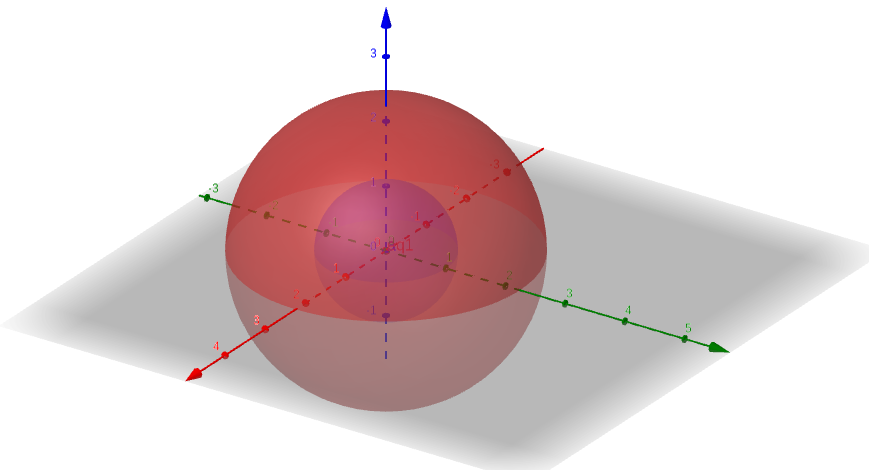
\includegraphics[scale=0.5]{img/ejercicios/1/16-j.png} 
\centering
\label{fig:1-16-j}
\end{figure}

Por lo tanto, el interior se obtiene relajando las desigualdades.

\begin{equation}
\tcboxmath[colback=orange!25!white,colframe=orange,title=1.16.j) Interior]
{ A^{\circ} = \{ (x,y,z) \in \Bbb R^3 / 1 < x^2 + y^2 + z^2 < 5 \} }
\end{equation}

Y la frontera está dada por las caras de las esferas:

\begin{equation}
\tcboxmath[colback=orange!25!white,colframe=orange,title=1.16.j) Frontera]
{
\begin{array}{ll}
\partial{A} = & \{ (x,y,z) \in \Bbb R^3 / x^2 + y^2 + z^2 = 1 \} \\
 & \cup \{ (x,y,z) \in \Bbb R^3 / x^2 + y^2 + z^2 = 5 \}
\end{array}
}
\end{equation}

\hrule
\vspace{10 pt}

\subsection*{1.17}
\label{subsec:1.17}
\addcontentsline{toc}{subsection}{\nameref{subsec:1.17}}

\textbf{Hallar cuando sea posible un punto exterior y un punto interior al conjunto dado. Analizar si es arco-conexo.} 

\begin{enumerate}[(a)]
\bfseries
\item $xy \geq 1$ (en $\Bbb R^2$)

\item $x + y = 1$ (en $\Bbb R^2$)

\item $x^2 + y^2 + (z-1)^2 = 0$ (en $\Bbb R^3$)

\item $(y - x^2 + 2) (y + x^2 -4) > 0$ (en $\Bbb R^2$)

\item $xyz < 0$ (en $\Bbb R^3$)

\item $2 < x <4, 2 < y \leq 5$ (en $\Bbb R^3$)
\end{enumerate}
\hrule

\subsubsection*{1.17.a}
\label{subsubsec:1.17.a}
\addcontentsline{toc}{subsubsection}{\nameref{subsubsec:1.17.a}}

Esta región ya se vio antes, en el ejercicio 1-11-g. Se repite su gráfico en la figura \ref{fig:1-17-a} por comodidad.

\begin{figure}[ht]
\caption{\textbf{17-a}}
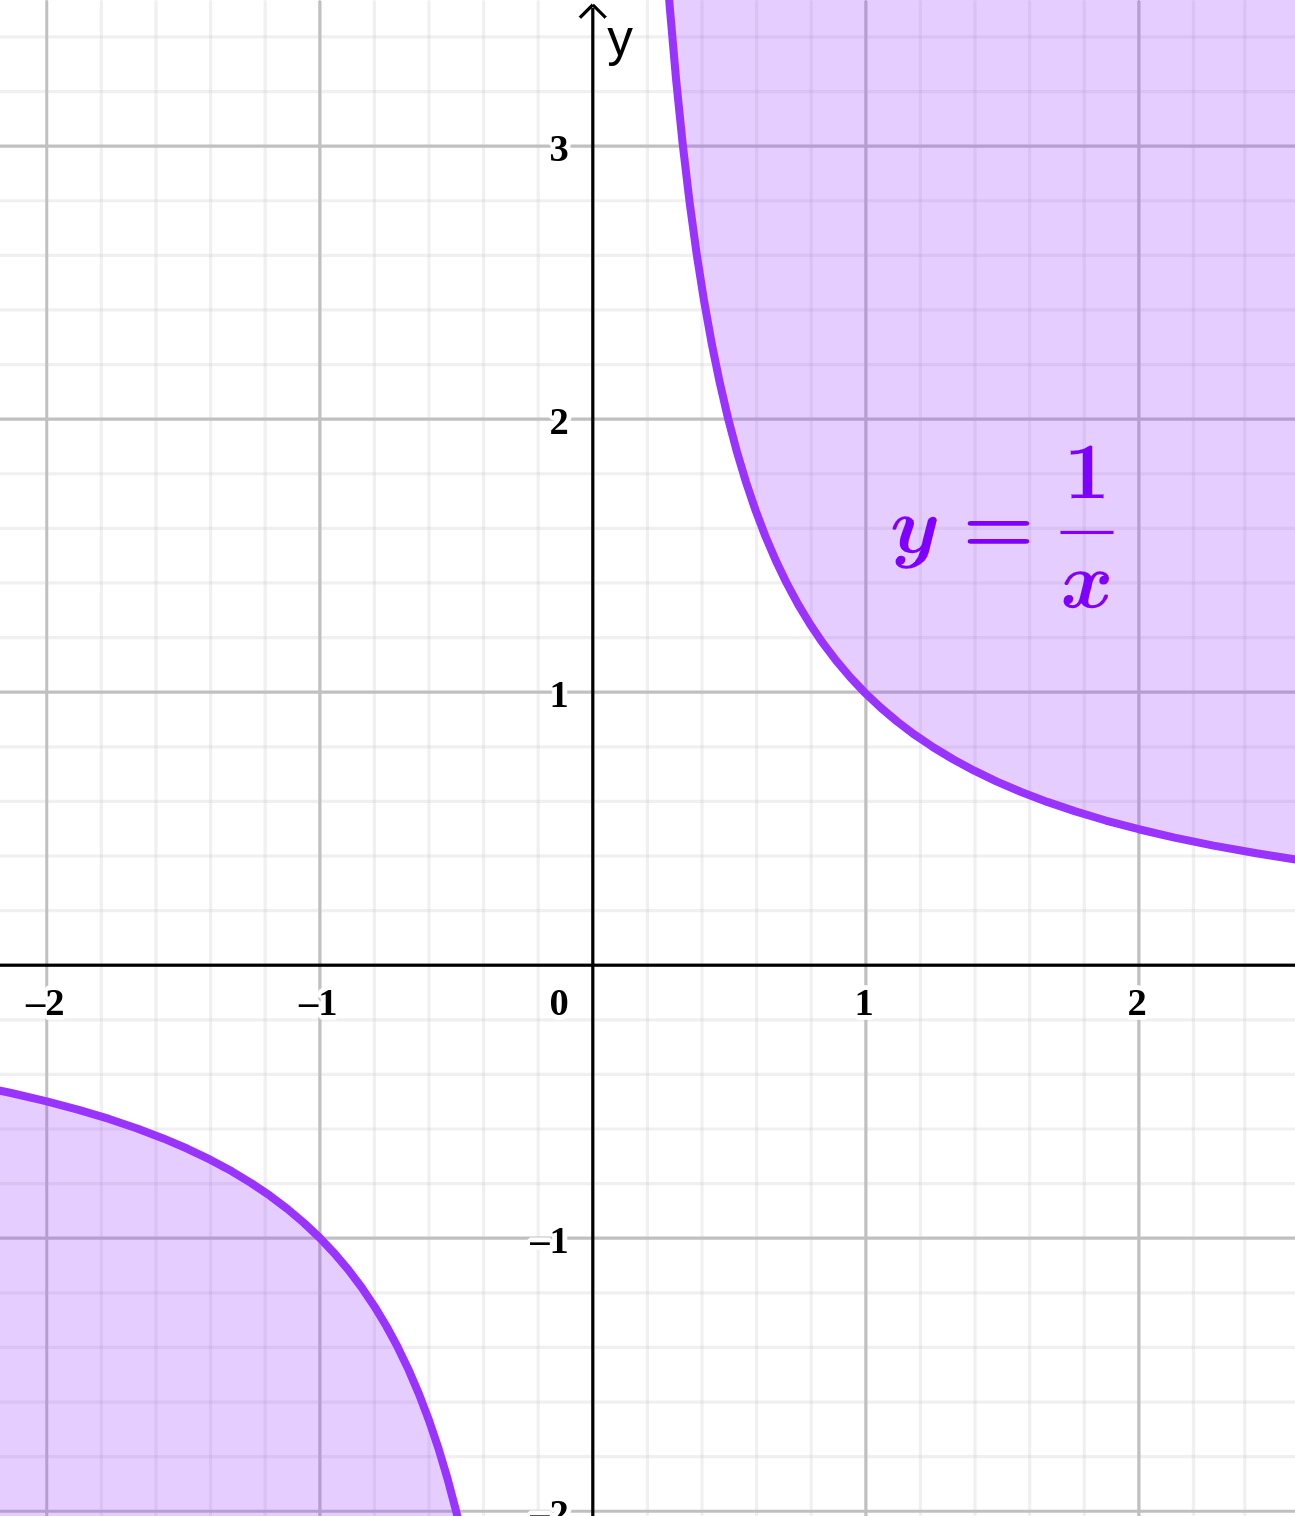
\includegraphics[scale=1]{img/ejercicios/1/11-g.png} 
\centering
\label{fig:1-17-a}
\end{figure}

Entonces, un interior $P_i$ y uno exterior $P_e$ pueden ser:

\begin{equation}
\tcboxmath[colback=orange!25!white,colframe=orange,title=1.17.a]
{
P_i = (2,2), P_e = (0, 0)
}
\end{equation}

En cuanto a si es arco-conexo, puede demostrarse que no lo es eligiendo los puntos $(-2,2)$ y $(2,2)$. No hay curva continua contenida en $A$ que los una.

\begin{equation}
\tcboxmath[colback=orange!25!white,colframe=orange,title=1.17.a]
{ \text{A NO es arco-conexo} }
\end{equation}

\subsubsection*{1.17.b}
\label{subsubsec:1.17.b}
\addcontentsline{toc}{subsubsection}{\nameref{subsubsec:1.17.b}}

El conjunto $A$ es la recta $y = -x + 1$. Cualquier punto de la recta sirve como punto interno, y cualquiera fuera de ella como punto externo.

\begin{equation}
\tcboxmath[colback=orange!25!white,colframe=orange,title=1.17.b]
{
P_i = (1, 0), P_e = (0, 0)
}
\end{equation}

Todo par de puntos en la recta puede ser unido por una curva continua: la propia recta. Ergo, es arco conexo.

\begin{equation}
\tcboxmath[colback=orange!25!white,colframe=orange,title=1.17.b]
{ \text{A es arco-conexo} }
\end{equation}

\subsubsection*{1.17.c}
\label{subsubsec:1.17.c}
\addcontentsline{toc}{subsubsection}{\nameref{subsubsec:1.17.c}}

Considérese $x^2 + y^2 + (z-1)^2 = 0$ como ecuación. Dado que los tres son cuadrados, son siempre positivos y la única solución en el dominio de los reales es que los tres sumandos sean cero: $x = 0, y = 0, z = 1$. Por ende, el conjunto $A$ consiste sólo del punto $(0, 0, 1)$. Ergo:

\begin{equation}
\tcboxmath[colback=orange!25!white,colframe=orange,title=1.17.c]
{
P_i = (0, 0, 1), P_e = (0, 0, 0)
}
\end{equation}

\begin{equation}
\tcboxmath[colback=orange!25!white,colframe=orange,title=1.17.c]
{ \text{A es arco-conexo} }
\end{equation}

\subsubsection*{1.17.d}
\label{subsubsec:1.17.d}
\addcontentsline{toc}{subsubsection}{\nameref{subsubsec:1.17.d}}

Dado que $A$ está expresado como producto de dos factores, y la desigualdad exige que dicho producto sea positivo, puede analizarse el signo del producto en base a los factores.

Caso 1: ambos factores son positivos.

\begin{equation}
\left\{ \begin{array}{ll}
y - x^2 + 2 > 0 \\
y + x^2 -4 > 0
\end{array}
\right. \Rightarrow \left\{ \begin{array}{ll}
y > x^2 - 2 \\
y > -x^2 + 4
\end{array}
\right.
\end{equation}

Caso 2: ambos factores son negativos.

\begin{equation}
\left\{ \begin{array}{ll}
y - x^2 + 2 < 0 \\
y + x^2 -4 < 0
\end{array}
\right. \Rightarrow \left\{ \begin{array}{ll}
y < x^2 - 2 \\
y < -x^2 + 4
\end{array}
\right.
\end{equation}

El conjunto $A$ consiste entonces en la unión de los conjuntos de ambos casos. Graficando en azul el caso 1 y en rojo el caso 2, se obtiene la figura .\ref{fig:1-17-d}.

\begin{figure}[ht]
\caption{\textbf{17-d}}
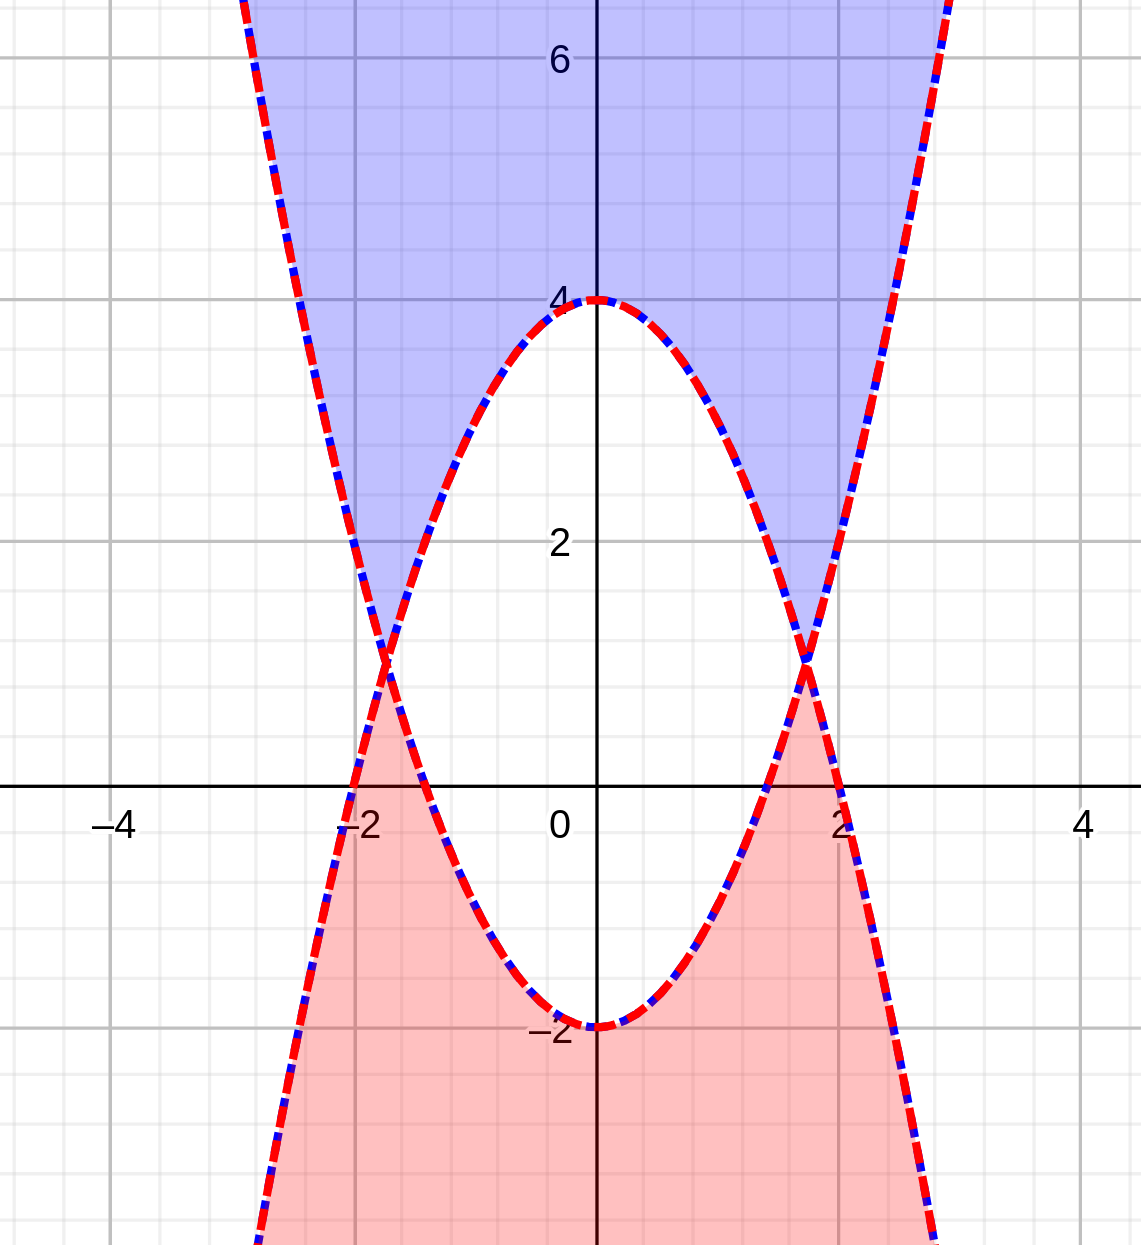
\includegraphics[scale=1]{img/ejercicios/1/17-d.png} 
\centering
\label{fig:1-17-d}
\end{figure}

Por lo tanto, un par posible de puntos interno y externo es:

\begin{equation}
\tcboxmath[colback=orange!25!white,colframe=orange,title=1.17.d]
{
P_i = (0, 6), P_e = (0, 0)
}
\end{equation}

El conjunto $A$ tiene dos regiones que se unen en dos puntos. Dichos puntos no pertenecen al conjunto, porque en ellos se anula el producto. Por lo tanto, si se elige un punto de la región azul y otro de la región roja, no existe curva continua contenida en $A$ que los una. Ergo,

\begin{equation}
\tcboxmath[colback=orange!25!white,colframe=orange,title=1.17.d]
{ \text{A NO es arco-conexo} }
\end{equation}

\subsubsection*{1.17.e}
\label{subsubsec:1.17.e}
\addcontentsline{toc}{subsubsection}{\nameref{subsubsec:1.17.e}}

La forma más directa de analizar este caso es considerar los 8 octantes del espacio tridimensional, y usar un árbol de decisión para determinar cuáles octantes pertenecen al conjunto. Dicho árbol puede visualizarse en la figura \ref{fig:1-17-e}. Los caminos verdes corresponden a tomar un valor positivo de la variable, y los rojos un valor negativo. Así, se obtienen las ocho combinaciones asociadas a los 8 octantes. El signo del triple producto se marca en el último nodo del árbol, con un signo más verde para producto positivo, y un triángulo invertido rojo para producto negativo.

\begin{figure}[ht]
\caption{\textbf{17-e}}
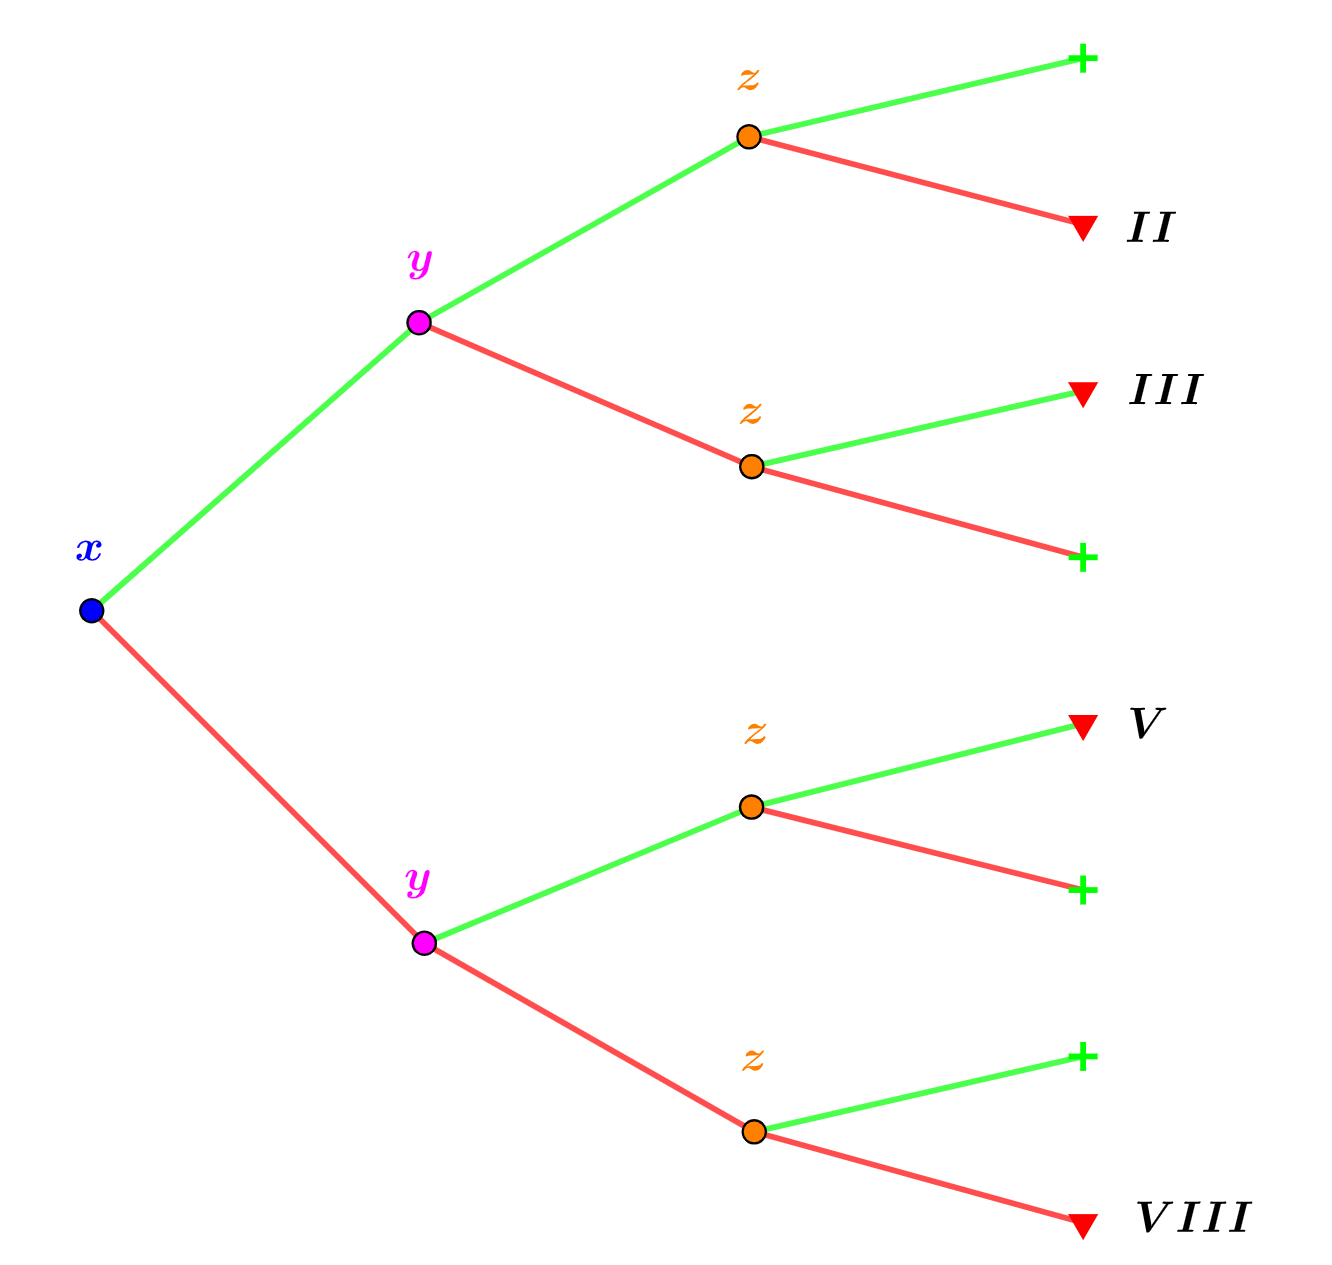
\includegraphics[scale=0.5]{img/ejercicios/1/17-e.png} 
\centering
\label{fig:1-17-e}
\end{figure}

Resulta entonces el conjunto A:

\begin{equation}
\begin{array}{ll}
A = & \{ (x,y,z) \in \Bbb R^3 / x > 0 \wedge y > 0 \wedge z < 0 \} \\
& \cup \{ (x,y,z) \in \Bbb R^3 / x > 0 \wedge y < 0 \wedge z > 0 \} \\
& \cup \{ (x,y,z) \in \Bbb R^3 / x < 0 \wedge y > 0 \wedge z > 0 \} \\
& \cup \{ (x,y,z) \in \Bbb R^3 / x < 0 \wedge y < 0 \wedge z < 0 \}
\end{array}
\end{equation}

Entonces, un par de posibles puntos interno y externo es:

\begin{equation}
\tcboxmath[colback=orange!25!white,colframe=orange,title=1.17.e]
{
P_i = (-1, -1, -1), P_e = (0, 0, 0)
}
\end{equation}

Las desigualdades son estrictas, lo cual excluye los ejes y el origen. Sin esas áreas de contacto, los octantes quedan desconectados entre sí. Un punto en un octante no puede ser unido con un punto de otro octante con una curva continua. Por lo tanto,

\begin{equation}
\tcboxmath[colback=orange!25!white,colframe=orange,title=1.17.e]
{ \text{A NO es arco-conexo} }
\end{equation}

\subsubsection*{1.17.f}
\label{subsubsec:1.17.f}
\addcontentsline{toc}{subsubsection}{\nameref{subsubsec:1.17.f}}

Como $z$ no aparece en las desigualdades, este caso puede analizarse en el plano $xy$ y el gráfico de dicho plano será el mismo para todo valor de $z$. Esto puede observarse en la figura \ref{fig:1-17-f}.

\begin{figure}[ht]
\caption{\textbf{17-f}}
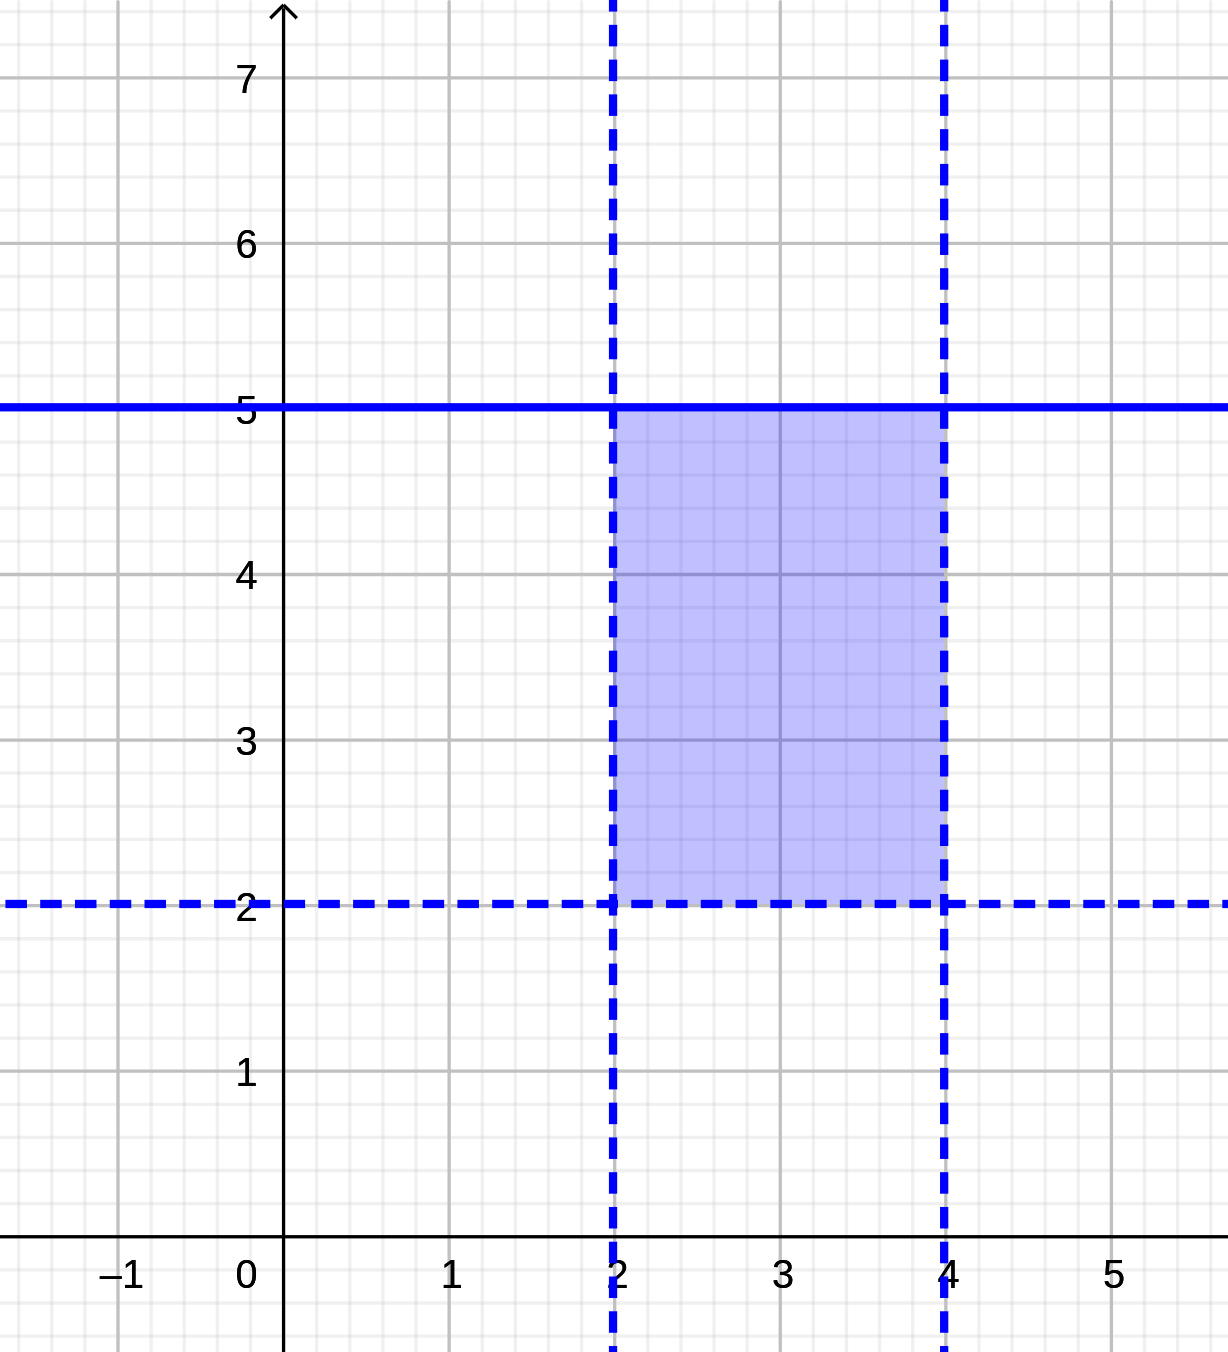
\includegraphics[scale=0.7]{img/ejercicios/1/17-f.png} 
\centering
\label{fig:1-17-f}
\end{figure}

Por lo tanto, el conjunto $A$ es una barra rectangular infinita paralela al eje $z$. Sólo una de sus caras, la asociada a $y = 5$, es parte del conjunto; las otras tres no pertenecen. Por ende, un par posible de puntos interno y externo es:

\begin{equation}
\tcboxmath[colback=orange!25!white,colframe=orange,title=1.17.f]
{
P_i = (3, 3, 0), P_e = (0, 0, 0)
}
\end{equation}

El interior de la región es un sólido continuo. Cualquier par de puntos interiores puede ser unido con una curva continua. Por ende,

\begin{equation}
\tcboxmath[colback=orange!25!white,colframe=orange,title=1.17.f]
{ \text{A es arco-conexo} }
\end{equation}

\hrule
\vspace{10 pt}

\subsection*{1.18}
\label{subsec:1.18}
\addcontentsline{toc}{subsection}{\nameref{subsec:1.18}}

\textbf{Describir mediante inecuaciones un conjunto plano $A$ tal que:} 

\begin{enumerate}[(a)]
\bfseries
\item Todo punto sea punto frontera.

\item Todo punto sea punto aislado.

\item $A - A^{\circ} = \{ (0, 0) \}$

\item $A$ es cerrado y su interior es $\{ (x,y): x^2 + y^2 < 1 \}$

\item $A$ es no acotado y su frontera es $\{ (x,y): |x| + |y| = 1 \}$
\end{enumerate}
\hrule

\subsubsection*{1.18.a}
\label{subsubsec:1.18.a}
\addcontentsline{toc}{subsubsection}{\nameref{subsubsec:1.18.a}}

Cualquier curva continua satisface que todos sus puntos sean frontera; cualquier entorno centrado en un punto de la curva contendrá puntos de $A$ y de $A^C$. Por ejemplo, una recta:

\begin{equation}
\tcboxmath[colback=orange!25!white,colframe=orange,title=1.18.a]
{ A = \{ (x,y) \in \Bbb R^2 / x + y = 1 \} }
\end{equation}

Con inecuaciones:

\begin{equation}
\tcboxmath[colback=orange!25!white,colframe=orange,title=1.18.a]
{ A = \left\{ (x,y) \in \Bbb R^2 / \left\{ \begin{array}{ll}
x + y \geq 1 \\
x + y \leq 1 
\end{array} \right. \right\} }
\end{equation}

\subsubsection*{1.18.b}
\label{subsubsec:1.18.b}
\addcontentsline{toc}{subsubsection}{\nameref{subsubsec:1.18.b}}

Cualquier conjunto formado por dos puntos (para cumplir con que sea más de uno) satisface esto; siempre existirá un entorno reducido centrado en dichos puntos tendrá intersección vacía con $A$.Por ejemplo:

\begin{equation}
\tcboxmath[colback=orange!25!white,colframe=orange,title=1.18.b]
{ A = \{ (x,y) \in \Bbb R^2 / (x,y) = (0,0) \vee (x,y) = (1,1) \} }
\end{equation}

Como en el inciso anterior, es trivial expresar esto con inecuaciones.

\begin{equation}
\tcboxmath[colback=orange!25!white,colframe=orange,title=1.18.b]
{
\begin{array}{ll}
A = \{ &(x,y) \in \Bbb R^2 / (x \geq 0 \wedge x \leq 0 \wedge y \geq 0 \wedge y \leq 0) \\
& \vee (x \geq 1 \wedge x \leq 1 \wedge y \geq 1 \wedge y \leq 1) \}
\end{array}
}
\end{equation}

\subsubsection*{1.18.c}
\label{subsubsec:1.18.c}
\addcontentsline{toc}{subsubsection}{\nameref{subsubsec:1.18.c}}

Para cumplir esta restricción, $A$ tiene que ser tal que su frontera consista sólo del origen. Un conjunto abierto con una ``esquina'' en el origen, al que se le agrega el origen como punto, cumple esto. Por ejemplo, el conjunto de la figura \ref{fig:1-18-c}.

\begin{figure}[ht]
\caption{\textbf{18-c}}
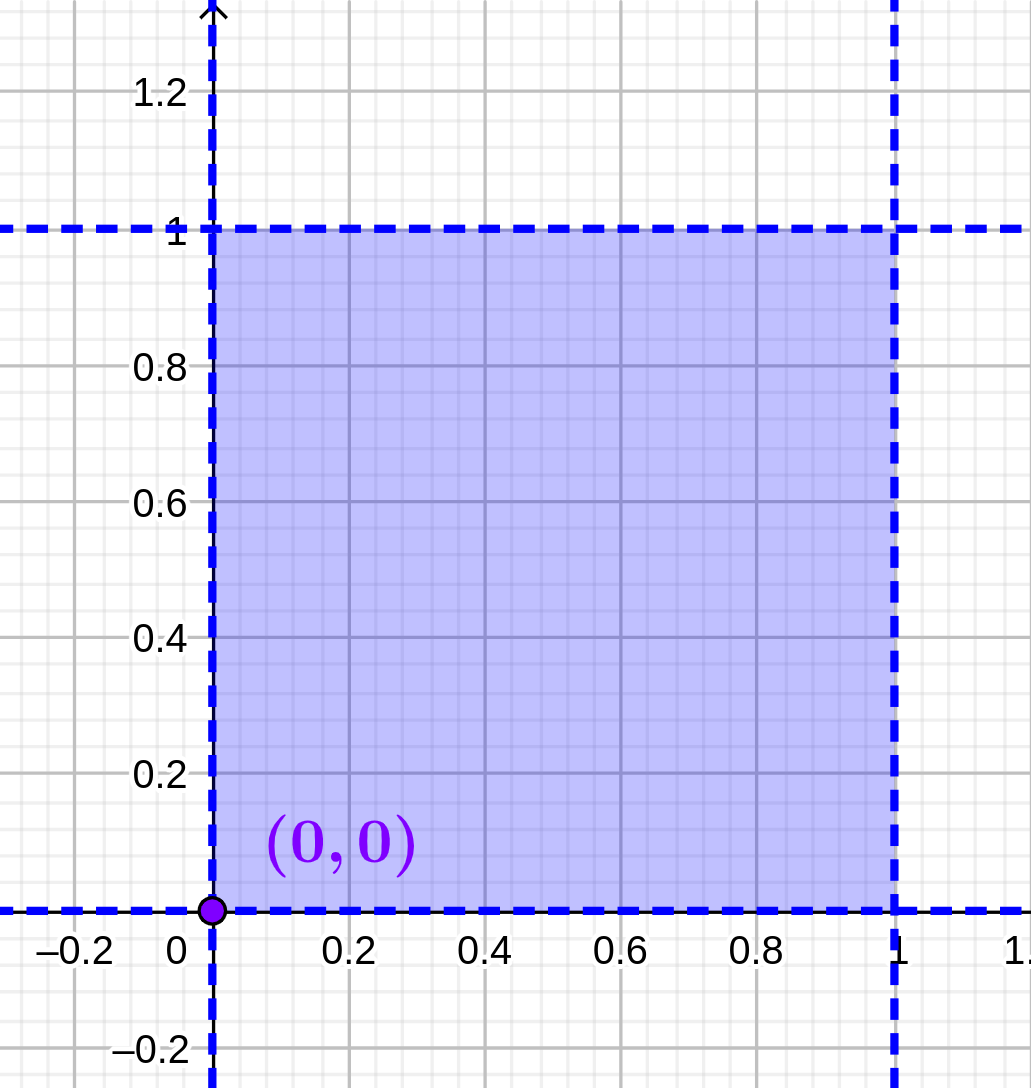
\includegraphics[scale=3.5]{img/ejercicios/1/18-c.png} 
\centering
\label{fig:1-18-c}
\end{figure}

Expresado con inecuaciones:

\begin{equation}
\tcboxmath[colback=orange!25!white,colframe=orange,title=1.18.c]
{
\begin{array}{ll}
A = \{ &(x,y) \in \Bbb R^2 / (0<x<1 \wedge 0<y<1) \\
& \vee (x \geq 0 \wedge x \leq 0 \wedge y \geq 0 \wedge y \leq 0) \}
\end{array}
}
\end{equation}

\subsubsection*{1.18.d}
\label{subsubsec:1.18.d}
\addcontentsline{toc}{subsubsection}{\nameref{subsubsec:1.18.d}}

El conjunto que satisface esto de forma más directa es el círculo de radio 1, incluyendo el borde. Es cerrado porque se cumple que $A = \overline{A} = A \cup \partial{A}$. La frontera es la circunferencia.

\begin{equation}
\tcboxmath[colback=orange!25!white,colframe=orange,title=1.18.d]
{ \{ (x,y) \in \Bbb R^2 / x^2 + y^2 \leq 1 \} }
\end{equation}

\subsubsection*{1.18.e}
\label{subsubsec:1.18.e}
\addcontentsline{toc}{subsubsection}{\nameref{subsubsec:1.18.e}}

En primer lugar, considérese el gráfico de $|x|+|y| = 1$. Despejando $|y|$:

\begin{equation}
|y| = -|x| + 1
\end{equation}

Para $y \geq 0$:

\begin{equation}
y = -|x| + 1
\end{equation}

Para $y < 0$:

\begin{equation}
y = |x| - 1
\end{equation}

Uniendo ambos casos, resulta la figura \ref{fig:1-18-e-01}. Un conjunto no acotado que tiene dichas curvas como frontera es el graficado en la figura \ref{fig:1-18-e-02}.

\begin{figure}[ht]
\caption{\textbf{18-e-01}}
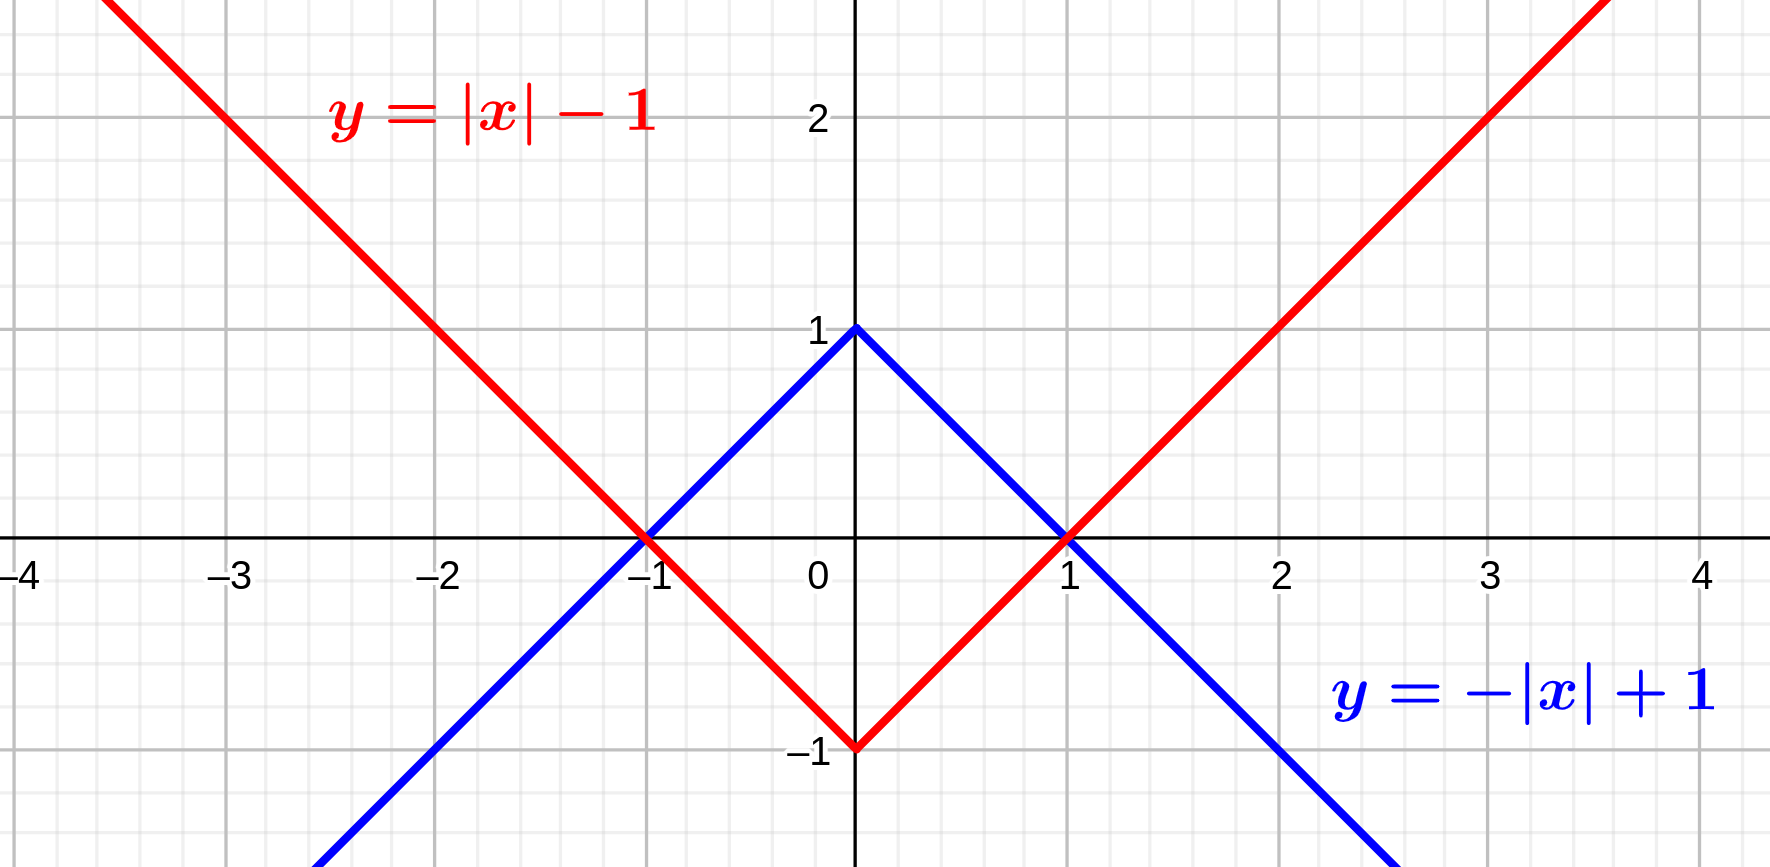
\includegraphics[scale=1]{img/ejercicios/1/18-e-01.png} 
\centering
\label{fig:1-18-e-01}
\end{figure}

\begin{figure}[ht]
\caption{\textbf{18-e-02}}
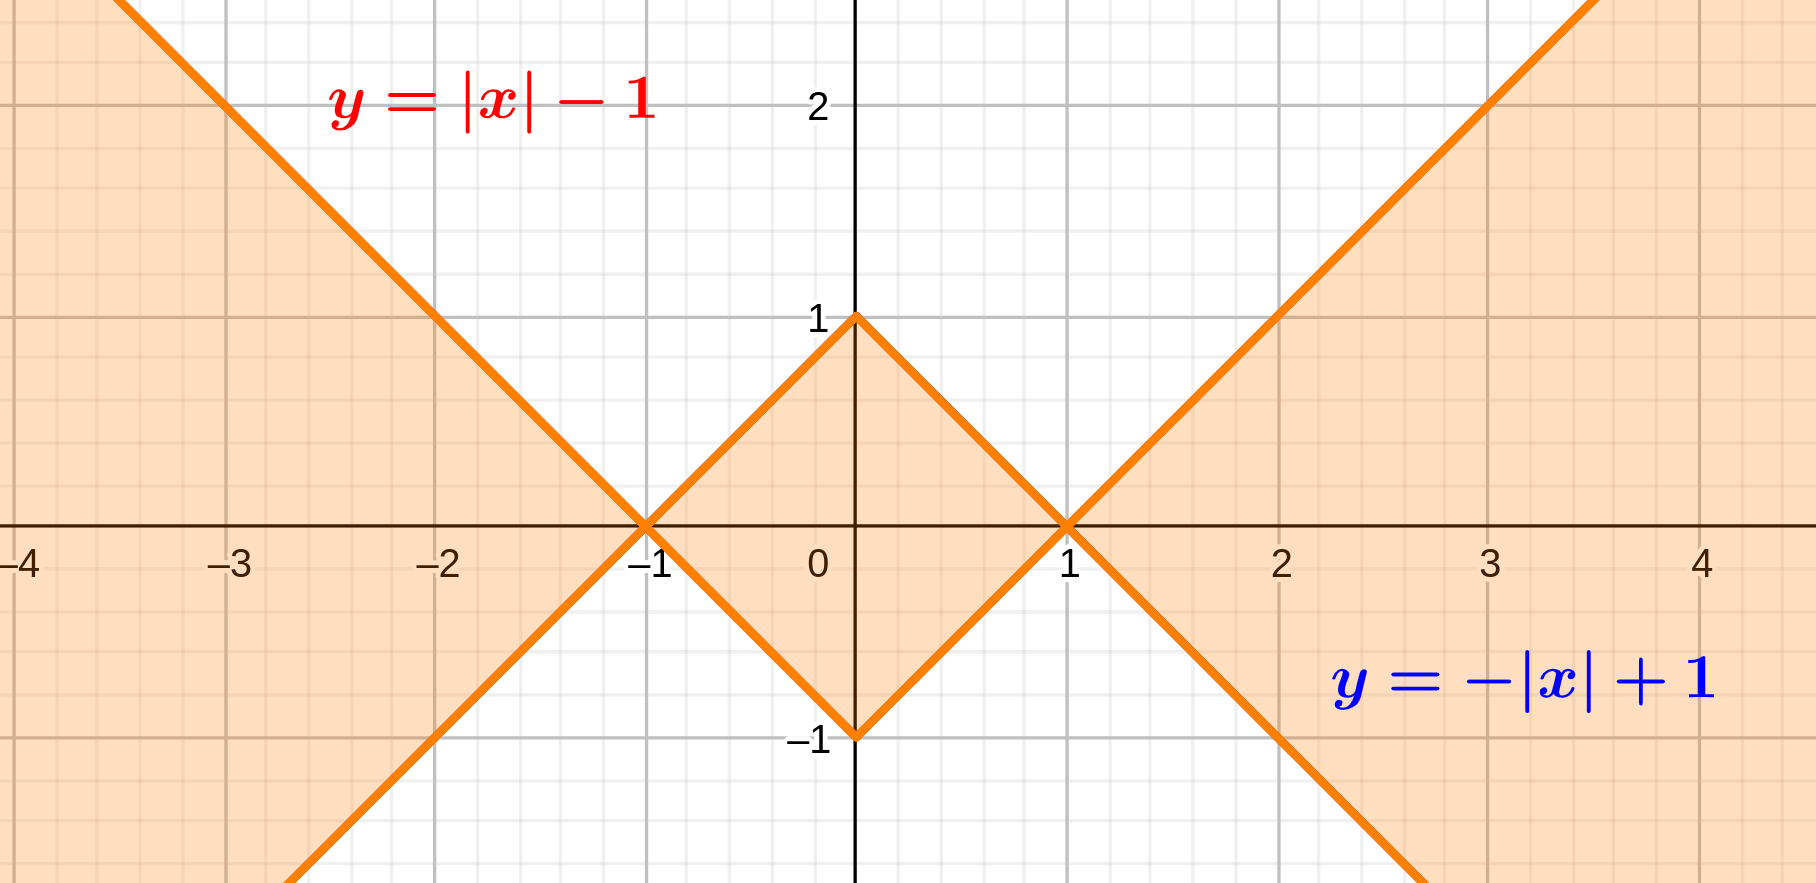
\includegraphics[scale=1]{img/ejercicios/1/18-e-02.png} 
\centering
\label{fig:1-18-e-02}
\end{figure}

Para describir ese conjunto con inecuaciones, conviene hacerlo por partes. En los sectores laterales infinitos ($|x| \geq 1$), se cumple una desigualdad, y en el centro ($|x| \leq 1$) otra.

\begin{equation}
\tcboxmath[colback=orange!25!white,colframe=orange,title=1.18.e]
{
\begin{array}{ll}
A = \{ &(x,y) \in \Bbb R^2 / -|x|+1 \leq y \leq |x|-1 \wedge |x| \geq 1 \} \\
& \cup \{ (x,y) \in \Bbb R^2 / |x|-1 \leq y \leq -|x|+1 \wedge |x| \leq 1 \}
\end{array}
}
\end{equation}

\bigskip

\section{Funciones, límite, continuidad, derivadas}

\hrule
\vspace{10 pt}

\subsection*{2.1}
\label{subsec:2.1}
\addcontentsline{toc}{subsection}{\nameref{subsec:2.1}}

\textbf{En los siguientes casos, describir el dominio de $f$, determinar si es un conjunto cerrado, abierto, o acotado; describir los conjuntos de nivel de $f$ y esbozar su gráfico.} 

\begin{enumerate}[(a)]
\bfseries
\item $f(x,y)=3 \left( 1 - \frac{x}{2} - \frac{y}{2} \right)$
\item $f(x,y)= \sqrt{y-x}$
\item $f(x,y)= \sqrt{4-x^2-y^2}$
\item $f(x,y)= 9x^2 + 4y^2$
\item $f(x,y)= x^2 - y^2$
\item $f(x,y)= \frac{1}{\sqrt{16 -x^2 -y^2}}$
\item $f(x,y)= 25 - x^2$
\item $f(x,y)= e^{-x^2-y^2}$
\item $f(x,y)= \sqrt{x^2 + 2y^2}$
\item $f(x,y)= \min(x, y)$
\item $f(x,y)= \max(x, y)$
\end{enumerate}
\hrule

\subsubsection*{2.1.a}
\label{subsubsec:2.1.a}
\addcontentsline{toc}{subsubsection}{\nameref{subsubsec:2.1.a}}

$x$ e $y$ pueden tomar cualquier combinación de valores sin causar ninguna indeterminación. Por ende,

\begin{equation}
\tcboxmath[colback=orange!25!white,colframe=orange,title=2.1.a]
{
\begin{array}{ll}
A = \mathop{Dom}(f) = \Bbb R^2 \\
\text{A NO es cerrado} \\
\text{A es abierto} \\
\text{A NO es acotado} \\
\end{array} 
}
\end{equation}

En cuanto a los conjuntos de nivel, observando la definición de $f$, es evidente que $z = f(x,y)$ puede tomar cualquier valor real. Por lo tanto, $\mathop{Img}(f) = \Bbb R$, y:

\begin{equation}
C_k(f) = \{ (x,y) \in \Bbb R^2 / 3(1-x/2-y/2) = k, k \in \Bbb \}
\end{equation}

Acomodando para expresar $y$ como función de $x$ con parámetro $k$, resulta:

\begin{equation}
\tcboxmath[colback=orange!25!white,colframe=orange,title=2.1.a]
{
C_k(f) = \{ (x,y) \in \Bbb R^2 / y = -x -\frac{2}{3}k + 2, k \in \Bbb \}
}
\end{equation}

Por lo tanto, los conjuntos de nivel de $f$ son rectas de pendiente $-1$ desplazadas verticalmente.

Finalmente, para graficar $f$, observando su definición, es un plano en $\Bbb R^3$:

\begin{equation}
z = 3 -\frac{3}{2} x - \frac{3}{2} y \Rightarrow -3 = -\frac{3}{2}x -\frac{3}{2}y -z \Rightarrow 6 = 3x +3y +2z 
\end{equation}

Considerando que 3 puntos determinan unívocamente un plano, para graficar alcanza con 3 puntos. Por ejemplo, fijando valores para $x$ e $y$ y calculando el $z$ resultante, se tiene:

\begin{equation}
\begin{array}{ll}
f(0,0) = 3 \Rightarrow (0, 0, 3) \in \mathop{Graf}(f) \\
f(2,0) = 0 \Rightarrow (2, 0, 0) \in \mathop{Graf}(f) \\
f(0,2) = 0 \Rightarrow (0, 2, 0) \in \mathop{Graf}(f)
\end{array}
\end{equation}

\begin{figure}[ht]
\caption{\textbf{2-1-a}}
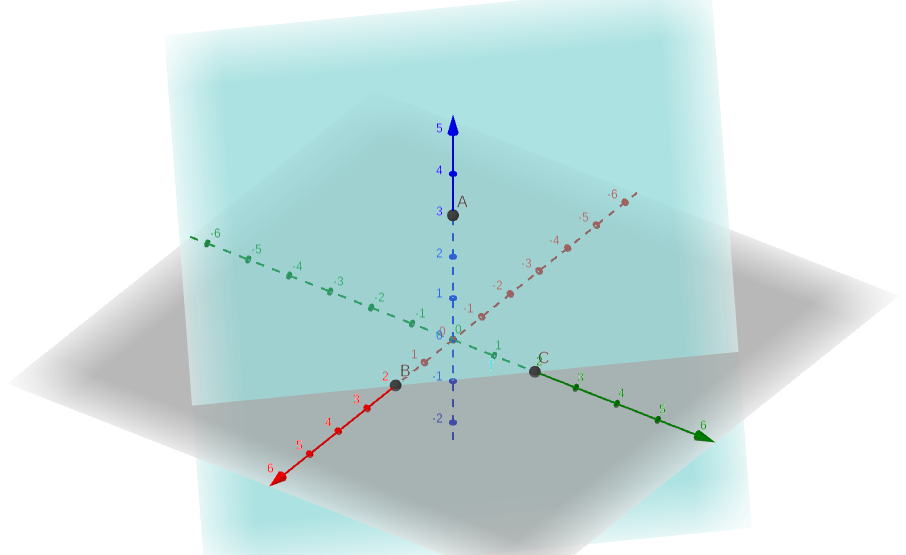
\includegraphics[scale=0.4]{img/ejercicios/2/1-a.png} 
\centering
\label{fig:2-1-a}
\end{figure}

\subsubsection*{2.1.b}
\label{subsubsec:2.1.b}
\addcontentsline{toc}{subsubsection}{\nameref{subsubsec:2.1.b}}

Dado que $z = \sqrt{y-x}$, para que la raíz cuadrada esté definida, debe ser $y-x \geq 0 \Rightarrow y \geq 0$. Por lo tanto:

\begin{equation}
\tcboxmath[colback=orange!25!white,colframe=orange,title=2.1.b]
{
\begin{array}{ll}
A = \mathop{Dom}(f) = \{ (x,y) \in \Bbb R^2 / y \geq x \} \\
\text{A es cerrado } (\overline{A} = A) \\
\text{A NO es abierto} (A^{\circ} \neq A) \\
\text{A NO es acotado} \\
\end{array} 
}
\end{equation}

La imagen de $f$ son cero y todos los reales positivos, por ser una raíz cuadrada. Por lo tanto, el conjunto de nivel $C_k(f)$ sólo está definido para $k \geq 0$, y consiste en:

\begin{equation}
C_k(f) = \{ (x,y) \in \Bbb R^2 / \sqrt{y-x} = k, k \in [0, +\infty) \}
\end{equation}

Despejando $y$ como función de $x$ parametrizada en $k$, resulta:

\begin{equation}
\tcboxmath[colback=orange!25!white,colframe=orange,title=2.1.b]
{
C_k(f) = \{ (x,y) \in \Bbb R^2 / y = x + k^2, k \in [0, +\infty) \}
}
\end{equation}

Así, los conjuntos de nivel son rectas de pendiente 1 desplazadas.

En cuanto al gráfico, si se piensa $z$ como una función de $y$ donde $x$ es un desplazamiento, se ve que la superficie $z$ está formada por curvas raíz cuadrada que nacen de la recta $y = x$ y crecen hacia el infinito. Véase la figura \ref{fig:1-2-b}.

\begin{figure}[ht]
\caption{\textbf{2-1-b}}
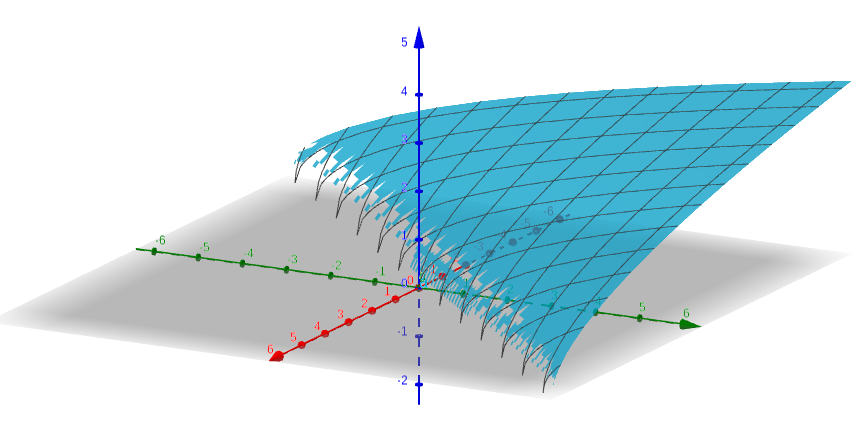
\includegraphics[scale=0.4]{img/ejercicios/2/1-b.png} 
\centering
\label{fig:2-1-b}
\end{figure}

\subsubsection*{2.1.c}
\label{subsubsec:2.1.c}
\addcontentsline{toc}{subsubsection}{\nameref{subsubsec:2.1.c}}

El dominio de $f$ estará dado por los valores que hagan cero o positivo el radicando: $4-x^2-y^2 \geq 0 \Leftrightarrow 4 \geq x^2 + y^2$. Ergo:

\begin{equation}
\tcboxmath[colback=orange!25!white,colframe=orange,title=2.1.c]
{
\begin{array}{ll}
A = \mathop{Dom}(f) = \{ (x,y) \in \Bbb R^2 / x^2 + y^2 \leq 4 \} \\
\text{A es cerrado } (\overline{A} = A) \\
\text{A NO es abierto } (A^{\circ} \neq A) \\
\text{A es acotado (totalmente contenido en un círculo de radio 3) } \\
\end{array} 
}
\end{equation}

Para los conjuntos de nivel, considérese primero la imagen de $f$. Su máximo valor corresponde al origen, ya que $(x,y) = (0,0)$ maximiza el radicando y por ende la raíz. En dicho caso, $z = 2$. Ahora bien, el dominio limita $x$ e $y$ de tal forma que el máximo valor que pueden tomar es $2$. En esos casos, $z = 0$. Por lo tanto, $Img(f) = [0, 2]$. Y los conjuntos de nivel resultan:

\begin{equation}
C_k(f) = \{ (x,y) \in \Bbb R^2 / \sqrt{4-x^2-y^2 = k}, 0 \leq k \leq 2 \}
\end{equation}

Estas curvas pueden expresarse como circunferencias, elevando su expresión al cuadrado miembro a miembro y acomodado:

\begin{equation}
\tcboxmath[colback=orange!25!white,colframe=orange,title=2.1.c]
{ C_k(f) = \{ (x,y) \in \Bbb R^2 / x^2+y^2 = 4-k^2, 0 \leq k \leq 2 \} }
\end{equation}

Para el gráfico, ya se saben varias cosas clave: el dominio es el interior del círculo de radio 2, $z$ varía entre 0 y 2, el máximo está en en el origen, y el mínimo en los bordes del círculo. Además, si los conjuntos de nivel son circunferencias, la superficie es una especie de cúpula circular. La figura \ref{fig:2-1-c} lo comprueba.

\begin{figure}[ht]
\caption{\textbf{2-1-c}}
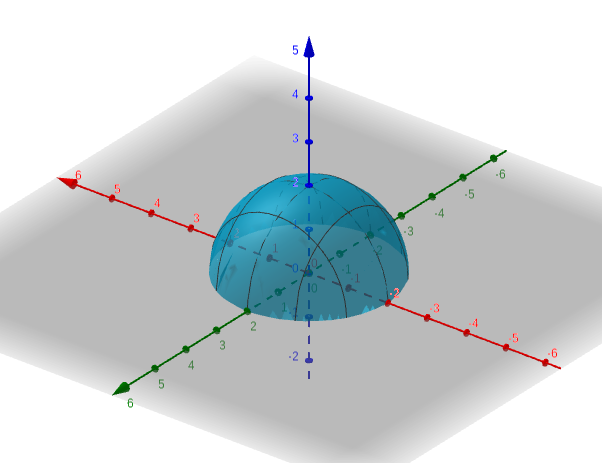
\includegraphics[scale=0.4]{img/ejercicios/2/1-c.png} 
\centering
\label{fig:2-1-c}
\end{figure}

\subsubsection*{2.1.d}
\label{subsubsec:2.1.d}
\addcontentsline{toc}{subsubsection}{\nameref{subsubsec:2.1.d}}

En este caso, el dominio es todo $\Bbb R^2$.

\begin{equation}
\tcboxmath[colback=orange!25!white,colframe=orange,title=2.1.d]
{
\begin{array}{ll}
A = \mathop{Dom}(f) = \Bbb R^2 \\
\text{A NO es cerrado} \\
\text{A es abierto} \\
\text{A NO es acotado} \\
\end{array} 
}
\end{equation}

En cuanto a la imagen, $z$ es la suma de dos cuadrados, por lo que sólo puede ser positivo: $\mathop{Img}(f) = [0, +\infty)$. Por lo tanto, los conjuntos de nivel serán:

\begin{equation}
C_k(f) = \{ (x,y) \in \Bbb R^2 / 9x^2 + 4 y^2 = k, k \in [0, +\infty] \}
\end{equation}

Observando fijo la expresión, corresponde a elipses cuyos semiejes crecen con $k$; y el de $x$ siempre es mayor.

\begin{equation}
\tcboxmath[colback=orange!25!white,colframe=orange,title=2.1.d]
{ C_k(f) = \left\{ (x,y) \in \Bbb R^2 / \frac{x^2}{ \left( \sqrt{\frac{k}{9}} \right)^2 } + \frac{y^2}{ \left(\sqrt{\frac{k}{4}}\right)^2 } = 1, k \in [0, +\infty] \right\} }
\end{equation}

Considerando que la imagen es $[0, +\infty)$, y los conjuntos de nivel son elipses, el gráfico de $f$ es un paraboloide elíptico, más ``estirado'' en la dirección $x$, por ser mayor ese semieje. La figura \ref{fig:2-1-d} demuestra esto.

\begin{figure}[ht]
\caption{\textbf{2-1-d}}
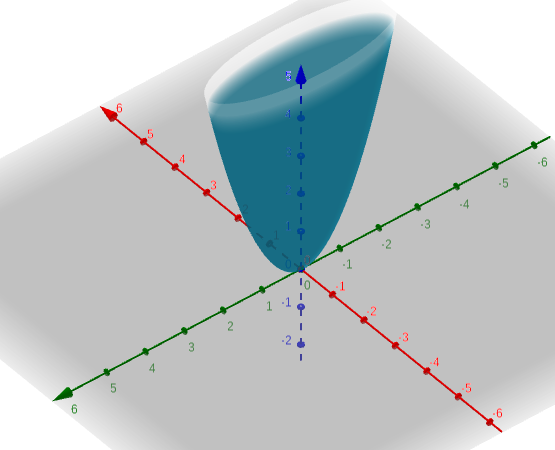
\includegraphics[scale=0.4]{img/ejercicios/2/1-d.png} 
\centering
\label{fig:2-1-d}
\end{figure}

\subsubsection*{2.1.e}
\label{subsubsec:2.1.e}
\addcontentsline{toc}{subsubsection}{\nameref{subsubsec:2.1.e}}

Para cualquier combinación de $x$ e $y$, $z$ está bien definido. Por ende:

\begin{equation}
\tcboxmath[colback=orange!25!white,colframe=orange,title=2.1.e]
{
\begin{array}{ll}
A = \mathop{Dom}(f) = \Bbb R^2 \\
\text{A NO es cerrado} \\
\text{A es abierto} \\
\text{A NO es acotado} \\
\end{array} 
}
\end{equation}

Considerando los conjuntos de nivel, la imagen de $f$ es todo $\Bbb R$. Y observando la expresión $x^2 - y^2 = k$, puede expresarse como hipérbolas (en tanto $k \neq 0$):

\begin{equation}
\tcboxmath[colback=orange!25!white,colframe=orange,title=2.1.e]
{ C_k(f) = \left\{ (x,y) \in \Bbb R^2 / \frac{x^2}{k} - \frac{y^2}{k} = 1, k \neq 0 \right\} }
\end{equation}

Nótese que para $k < 0$, se intercambian los signos de los sumandos, y por ende la simetría pasa del eje $y$ al $x$. 

El conjunto $C_0(f)$ corresponde a $x^2 - y^2 = 0 \Leftrightarrow x^2 = y^2 \Leftrightarrow |y| = |x|$. Para $y \geq 0$, es la curva $y = |x|$. Y para $y < 0$, es $y = -|x|$.

\begin{equation}
\tcboxmath[colback=orange!25!white,colframe=orange,title=2.1.e]
{ C_0(f) = \left\{ (x,y) \in \Bbb R^2 / y = |x| \text{ para } y \geq 0, y = -|x| \text{ para } y < 0 \right\} }
\end{equation}

Considerando que los conjuntos de nivel son las diagonales en $z = 0$, e hipérbolas de separación entre curvas creciente con $k$, el gráfico de $f$ es un paraboloide hiperbólico con punto silla en el origen. La simetría cambia para $z < 0$ como se vio al analizar $C_k(f)$. Ver figura \ref{fig:2-1-e}.

\begin{figure}[ht]
\caption{\textbf{2-1-e}}
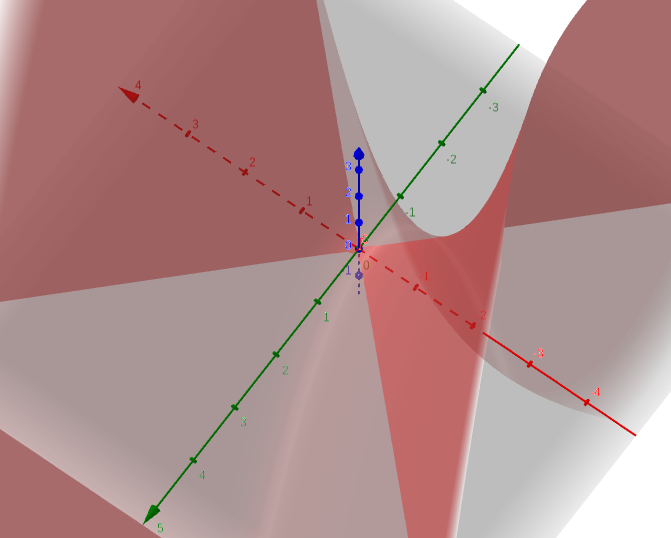
\includegraphics[scale=0.4]{img/ejercicios/2/1-e.png} 
\centering
\label{fig:2-1-e}
\end{figure}

\subsubsection*{2.1.f}
\label{subsubsec:2.1.f}
\addcontentsline{toc}{subsubsection}{\nameref{subsubsec:2.1.f}}

Para que $f$ esté bien definida en los reales, debe ser $16-x^2-y^2 > 0$  (el igual se quita para no dividir por cero). Entonces:

\begin{equation}
\tcboxmath[colback=orange!25!white,colframe=orange,title=2.1.f]
{
\begin{array}{ll}
A = \mathop{Dom}(f) = \{ (x,y) \in \Bbb R^2 / x^2 + y^2 < 16 \} \\
\text{A NO es cerrado} \\
\text{A es abierto} \\
\text{A es acotado} \\
\end{array} 
}
\end{equation}

La imagen de $f$ tiene su minímo en el origen, porque se maximiza el numerador. En dicho caso, $z = \frac{1}{4}$. A medida que los puntos se acercan al círculo de radio 4, el numerador se acerca a $0^+$, y por ende $z$ tiende a $+\infty$. Los conjuntos de nivel son entonces:

\begin{equation}
C_k(f) = \{ (x,y) \in \Bbb R^2 / \frac{1}{\sqrt{16-x^2-y^2}} = k, k \geq \frac{1}{4} \}
\end{equation}

Elevando al cuadrado miembro a miembro y acomodando, los $C_k$ resultan circunferencias:

\begin{equation}
\tcboxmath[colback=orange!25!white,colframe=orange,title=2.1.e]
{ C_k(f) = \{ (x,y) \in \Bbb R^2 / x^2 + y^2 = 16 -\frac{1}{k^2}, k \geq \frac{1}{4} \} }
\end{equation}

Considerando los conjuntos de nivel, el gráfico comienza en $z = \frac{1}{4}$, donde es sólo un punto. Para mayor $z$, son circunferencias que tienden rápidamente hacia la circunferencia de radio 4, pero jamás la alcanzan porque hay un infinitésimo restando. Por lo tanto, la superficie de $z=f(x,y)$ tiene forma de paraboloide; tiene su mínimo en $(0, 0, \frac{1}{4})$ y crece hacia infinito positivo, pero sin salirse del cilindro de radio $4$. La figura \ref{fig:2-1-f} corrobora esto.

\begin{figure}[ht]
\caption{\textbf{2.1.f}}
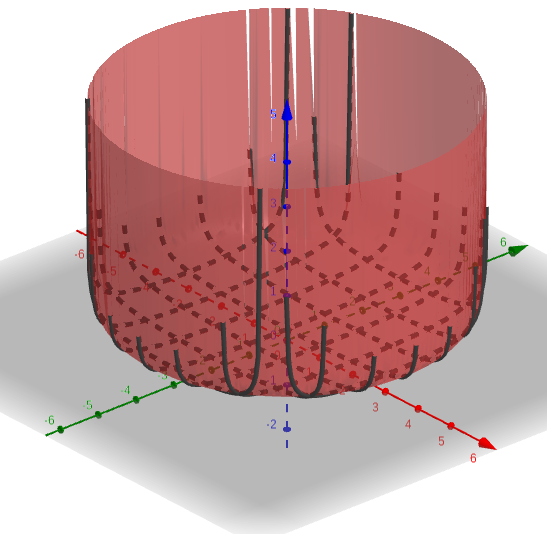
\includegraphics[scale=0.4]{img/ejercicios/2/1-f.png} 
\centering
\label{fig:2-1-f}
\end{figure}

\subsubsection*{2.1.g}
\label{subsubsec:2.1.g}
\addcontentsline{toc}{subsubsection}{\nameref{subsubsec:2.1.g}}

La función $f$ está definida para todo valor; por lo tanto,

\begin{equation}
\tcboxmath[colback=orange!25!white,colframe=orange,title=2.1.g]
{
\begin{array}{ll}
A = \mathop{Dom}(f) = \Bbb R^2 \\
\text{A NO es cerrado} \\
\text{A es abierto} \\
\text{A NO es acotado} \\
\end{array} 
}
\end{equation}

La imagen es $(-\infty, 25]$, ya que el valor mínimo que puede tomar $-x^2$ es cero. Por ende, los conjuntos de nivel son:

\begin{equation}
C_k(f) = \{ (x,y) \in \Bbb R^2 / 25-x^2 = k, k \leq 25 \}
\end{equation}

Despejando $x$, resulta: 

\begin{equation}
\tcboxmath[colback=orange!25!white,colframe=orange,title=2.1.g]
{ C_k(f) = \{ (x,y) \in \Bbb R^2 / x = \pm \sqrt{25-k}, k \leq 25 \} }
\end{equation}

Ergo, los conjuntos de nivel son pares de rectas paralelas y equidistantes al eje $x$. Para visualizar el gráfico, considérese que $y$ es una variable libre. La curva que ocurra en el plano $y = 0$ será idéntica para cualquier otro valor de $y$. Por lo tanto, observando el plano $xz$ en $y=0$, se tiene una simple parábola invertida, que alcanza su máximo en $x=0, z=25$, y corta al eje $x$ en $x=\pm5$. Replicando esa curva a lo largo del eje $y$, se obtiene la superficie de la figura \ref{fig:2-1-g}.

\begin{figure}[ht]
\caption{\textbf{2.1.g}}
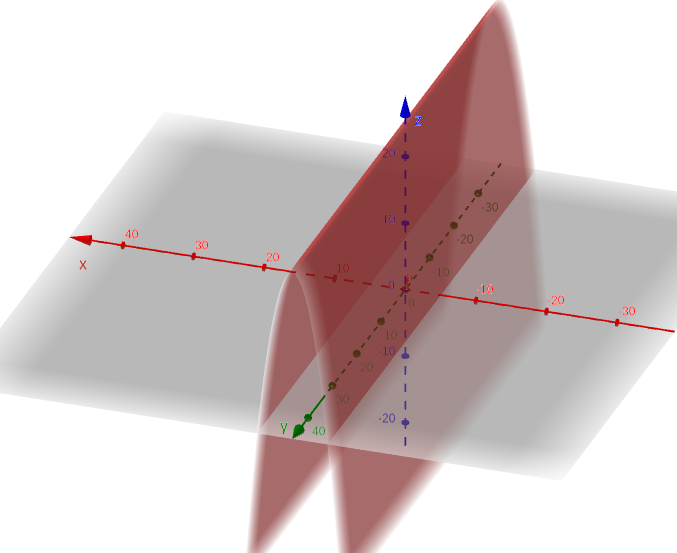
\includegraphics[scale=0.4]{img/ejercicios/2/1-g.png} 
\centering
\label{fig:2-1-g}
\end{figure}

\subsubsection*{2.1.h}
\label{subsubsec:2.1.h}
\addcontentsline{toc}{subsubsection}{\nameref{subsubsec:2.1.h}}

La función $f(x,y)$ está definida para toda combinación de $x$ e $y$. Ergo:

\begin{equation}
\tcboxmath[colback=orange!25!white,colframe=orange,title=2.1.h]
{
\begin{array}{ll}
A = \mathop{Dom}(f) = \Bbb R^2 \\
\text{A NO es cerrado} \\
\text{A es abierto} \\
\text{A NO es acotado} \\
\end{array} 
}
\end{equation}

La imagen de $f$ corresponde a una exponencial real cuyo exponente siempre es cero o negativo (por los cuadrados negados). Por lo tanto, el máximo valor que puede tomar es 1, en el origen. Para otros valores, tenderá a cero. Por ende, $\mathop{Img}(f) = (0, 1]$. Y los conjuntos de nivel están dados por:

\begin{equation}
C_k(f) = \{ (x,y) \in \Bbb R^2 / e^{-x^2-y^2} = k, 0 < k \leq 1 \}
\end{equation}

Aplicando la función $\ln$ miembro a miembro y acomodando, se ve que estas curvas son circunferencias.

\begin{equation}
\tcboxmath[colback=orange!25!white,colframe=orange,title=2.1.h]
{ C_k(f) = \left\{ (x,y) \in \Bbb R^2 / x^2+y^2 = \ln \left( \frac{1}{k} \right), 0 < k \leq 1 \right\} }
\end{equation}

Considerando la imagen y los conjuntos de nivel, el gráfico de $f$ debería ser como una campana de Gauss en las direcciones de $x$ e $y$, con su máximo en el origen y tendiendo a cero de forma rápida pero suave. La figura \ref{fig:2-1-h} corrobora esto.

\begin{figure}[ht]
\caption{\textbf{2.1.h}}
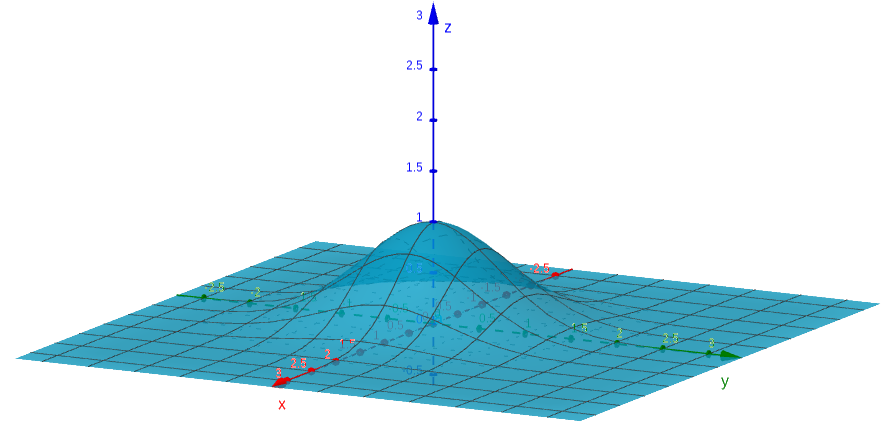
\includegraphics[scale=0.4]{img/ejercicios/2/1-h.png} 
\centering
\label{fig:2-1-h}
\end{figure}

\subsubsection*{2.1.i}
\label{subsubsec:2.1.i}
\addcontentsline{toc}{subsubsection}{\nameref{subsubsec:2.1.i}}

El radicando eleva $x$ e $y$ al cuadrado, lo cual impide que sea negativo. Por lo tanto, $f$ está definida para todo $\Bbb R^2$.

\begin{equation}
\tcboxmath[colback=orange!25!white,colframe=orange,title=2.1.i]
{
\begin{array}{ll}
A = \mathop{Dom}(f) = \Bbb R^2 \\
\text{A NO es cerrado} \\
\text{A es abierto} \\
\text{A NO es acotado} \\
\end{array} 
}
\end{equation}

La imagen de $f$ tiene que ser cero o positiva por ser una raíz cuadrada de valores entre 0 y $+\infty$: $Im(f) = [0, +\infty]$. Los conjuntos de nivel resultan entonces:

\begin{equation}
C_k(f) = \{ (x,y) \in \Bbb R^2 / \sqrt{x^2 + 2y^2} = k, k \geq 0 \}
\end{equation}

Elevando al cuadrado miembro a miembro, se ve que estas curvas son elipses. Acomodando para reflejar eso:

\begin{equation}
\tcboxmath[colback=orange!25!white,colframe=orange,title=2.1.i]
{
\begin{array}{ll}
C_k(f) = \left\{ (x,y) \in \Bbb R^2 / \frac{x^2}{k^2} + \frac{y^2}{\frac{k^2}{2}} = 1, k > 0 \right\} \\
C_0(f) = (0, 0)
\end{array}
}
\end{equation}

Considerando la imagen y conjuntos de nivel, el gráfico debería ser una especie de paraboloide elíptico, cuyo mínimo está en el origen, y crece hacia infinito. El ancho en $x$ será siempre el doble que en $y$, por las relaciones entre los semiejes. La figura \ref{fig:2-1-i} confirma esto, con un agregado: los radios de las elipses crecen linealmente con $z$; visualmente, la superficie es más un cono que un paraboloide. Esto tiene sentido observando que en $C_k(f)$, $k$ está elevado al cuadrado, igual que $x$ e $y$.

\begin{figure}[ht]
\caption{\textbf{2.1.i}}
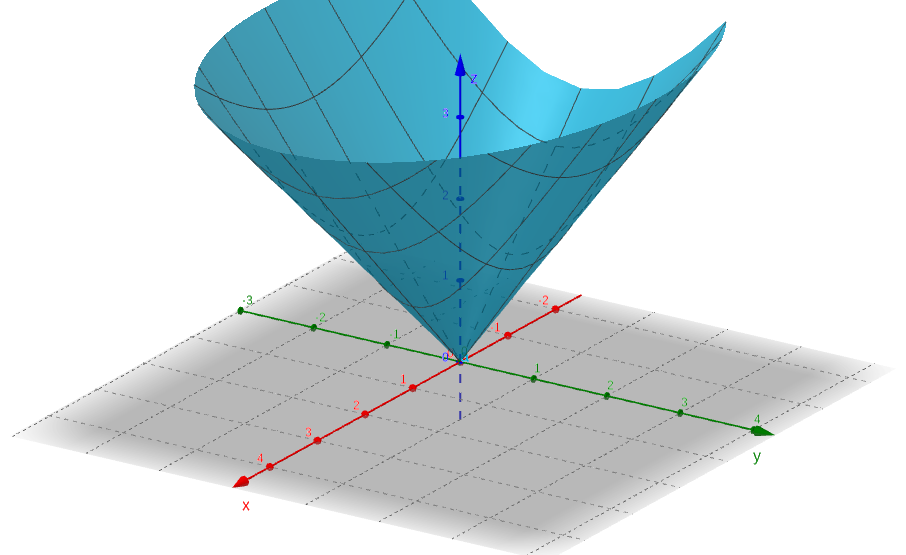
\includegraphics[scale=0.4]{img/ejercicios/2/1-i.png} 
\centering
\label{fig:2-1-i}
\end{figure}

\subsubsection*{2.1.j}
\label{subsubsec:2.1.j}
\addcontentsline{toc}{subsubsection}{\nameref{subsubsec:2.1.j}}

No hay ninguna combinación de $x$ e $y$ que cause alguna indeterminación; $f$ siempre está bien definida. Por lo tanto:

\begin{equation}
\tcboxmath[colback=orange!25!white,colframe=orange,title=2.1.j]
{
\begin{array}{ll}
A = \mathop{Dom}(f) = \Bbb R^2 \\
\text{A NO es cerrado} \\
\text{A es abierto} \\
\text{A NO es acotado} \\
\end{array} 
}
\end{equation}

La imagen es claramente todo $\Bbb R$, ya que $x$ e $y$ pueden tomar cualquier valor. En cuanto a los conjuntos de nivel, su planteo por definición sería:

\begin{equation}
C_k(f) = \{ (x,y) \in \Bbb R^2 / \min(x,y) = k, k \in \Bbb R \}
\end{equation}

Para cada valor fijo $k$, hay 3 puntos que satisfacen la igualdad:

\begin{equation}
\begin{array}{ll}
(k, k, k) \text{ si } x = y \\
(x, k, k) \text{ si } y < x \\
(k, y, k) \text{ si } x < y
\end{array}
\end{equation}

Por lo tanto, cada conjunto de nivel es un trío de puntos:

\begin{equation}
\tcboxmath[colback=orange!25!white,colframe=orange,title=2.1.j]
{ C_k(f) = \{ (x,y) \in \Bbb R^2 / (x,y)=(k,k) \vee (x,y)=(x,k) \vee (x,y)=(k,y), k \in \Bbb R \} }
\end{equation}

Para el gráfico, en esta ocasión los conjuntos de nivel no ayudan mucho. Considérese el plano dominio, $xy$; el valor que toma $z = f(x,y)$ está divido por la recta $y=x$. En la región de $\Bbb R^2$ donde $y <= x$, $z = y$, y para $y < x$, $z = x$. Ergo, $f$ puede expresarse de la siguiente manera:

\begin{equation}
z = f(x,y) = \left\{ \begin{array}{ll}
y \text{ si } y \leq x \\
x \text{ si } y > x
\end{array} \right.
\end{equation}

Ambas ramas de $f$ pueden considerarse como planos. Más concretamente, el plano $z = y$ es la recta $z = y$ en el plano $zy$, replicada a lo largo del eje $x$. Análogamente, el plano $z = x$ es la recta $z = x$ replicada a lo largo del eje $y$. Con esto en mente, el gráfico de $f$ se construye tomando las secciones de ambos planos correspondientes a cada región, y considerando que los planos se intersectan en la recta $y = x$. Esto es consistente con que los conjuntos de nivel sean tríos de puntos: un punto en el plano $z = y$, otro en el plano $z = x$, y otro sobre la recta donde se cortan los planos.

\begin{figure}[ht]
\caption{\textbf{2.1.j}}
\includegraphics[scale=0.4]{img/ejercicios/2/1-j.png} 
\centering
\label{fig:2-1-j}
\end{figure}

En la figura \ref{fig:2-1-j}, el plano $z = y$ se halla graficado en color cian, y el plano $z = x$ en rojo. La región $y \leq x$ en el plano $z = 0$ se halla marcada con una grilla a modo de referencia. Gracias a dicha referencia, es sencillo ver que el gráfico de $f$ corresponde a las mitades ``decrecientes'' de los planos demarcados por la recta $y = x$ y su proyección. Burdamente, el gráfico de $f$ es como un techo a dos aguas.

\subsubsection*{2.1.k}
\label{subsubsec:2.1.k}
\addcontentsline{toc}{subsubsection}{\nameref{subsubsec:2.1.k}}

Aplicando el mismo razonamiento que en el inciso anterior, con la única diferencia de tomar el máximo en lugar del mínimo:

\begin{equation}
\tcboxmath[colback=orange!25!white,colframe=orange,title=2.1.k]
{
\begin{array}{ll}
A = \mathop{Dom}(f) = \Bbb R^2 \\
\text{A NO es cerrado} \\
\text{A es abierto} \\
\text{A NO es acotado} \\
\end{array} 
}
\end{equation}

\begin{equation}
\tcboxmath[colback=orange!25!white,colframe=orange,title=2.1.j]
{ C_k(f) = \{ (x,y) \in \Bbb R^2 / (x,y)=(k,k) \vee (x,y)=(x,k) \vee (x,y)=(k,y), k \in \Bbb R \} }
\end{equation}

La definición por partes de $f$ intercambia los semiplanos:

\begin{equation}
z = f(x,y) = \left\{ \begin{array}{ll}
x \text{ si } y \leq x \\
y \text{ si } y > x
\end{array} \right.
\end{equation}

Por lo tanto, tomando como referencia la figura \ref{fig:2-1-j}, el gráfico de $f$ corresponde a las secciones ``crecientes'' de los planos $z = x$ y $z = y$. Es un techo a dos aguas invertido.

\hrule
\vspace{10 pt}

\subsection*{2.2}
\label{subsec:2.2}
\addcontentsline{toc}{subsection}{\nameref{subsec:2.2}}

\textbf{En los siguientes casos hallar, si existe, el límite indicado; en los casos en que no existe, fundamentar.} 

\begin{enumerate}[(a)]
\bfseries
\item $ \lim_{(x,y) \rightarrow (1,-1)} xy - y^2 $
\item $ \lim_{(x,y) \rightarrow (0,0)} \frac{x^2 + y^2}{y} $
\item $ \lim_{(x,y) \rightarrow (0,0)} \sqrt{x^2 + y^2} $
\item $ \lim_{(x,y) \rightarrow (1,-2)} x^2 + (y-2)^2 x $
\item $ \lim_{(x,y) \rightarrow (0,2)} \frac{y^2 (x-2)^2}{x^2 + (y-2)^2} $
\item $ \lim_{(x,y) \rightarrow (0,4)} \frac{x}{\sqrt{y}} $
\item $ \lim_{(x,y) \rightarrow (1,-2)} \left( xy, \frac{y}{x+1}, \sqrt{x^2 + y^2} \right) $
\item $ \lim_{(x,y,z) \rightarrow (0,1,1)} \frac{y+1}{\sqrt{z^2 - 1}} $
\item $ \lim_{(x,y) \rightarrow (0,0)} \left( y \cos\left(\frac{1}{x}\right), \frac{\sin(3x)}{2x}, x-y \right) $
\end{enumerate}
\hrule

\subsubsection*{2.2.a}
\label{subsubsec:2.2.a}
\addcontentsline{toc}{subsubsection}{\nameref{subsubsec:2.2.a}}

La función $f(x,y) = xy - x^2$ es continua en todo $\Bbb R^2$. Por lo tanto:

\begin{equation}
\tcboxmath[colback=orange!25!white,colframe=orange,title=2.2.a]
{ \lim_{(x,y) \rightarrow (1,-1)} f(x,y) = f(1,-1) = -2 }
\end{equation}

\subsubsection*{2.2.b}
\label{subsubsec:2.2.b}
\addcontentsline{toc}{subsubsection}{\nameref{subsubsec:2.2.b}}

Esta función tiene una singularidad en $(0, 0)$. Probando con los límites sucesivos:

\begin{align}
l_{12} = \lim_{y \rightarrow 0} \left( \lim_{x \rightarrow 0} \frac{x^2 + y^2}{y} \right) = \lim_{y \rightarrow 0} y = 0 \\
l_{21} = \lim_{x \rightarrow 0} \left( \lim_{y \rightarrow 0} \frac{x^2 + y^2}{y} \right) = \lim_{x \rightarrow 0} \infty
\end{align}

Si el límite existe, tiene que ser único. Por lo tanto, que difieran los límites sucesivos garantiza que:

\begin{equation}
\tcboxmath[colback=orange!25!white,colframe=orange,title=2.2.b]
{ \lim_{(x,y) \rightarrow (0,0)} \frac{x^2 + y^2}{y} = \nexists }
\end{equation}

\subsubsection*{2.2.c}
\label{subsubsec:2.2.c}
\addcontentsline{toc}{subsubsection}{\nameref{subsubsec:2.2.c}}

No hay singularidades en $f$.

\begin{equation}
\tcboxmath[colback=orange!25!white,colframe=orange,title=2.2.c]
{ \lim_{(x,y) \rightarrow (0,0)} \sqrt{x^2 + y^2} = 0 }
\end{equation}

\subsubsection*{2.2.d}
\label{subsubsec:2.2.d}
\addcontentsline{toc}{subsubsection}{\nameref{subsubsec:2.2.d}}

No hay singularidades en $f$.

\begin{equation}
\tcboxmath[colback=orange!25!white,colframe=orange,title=2.2.d]
{ \lim_{(x,y) \rightarrow (1,-2)} x^2 + (y-2)^2 x = 5 }
\end{equation}

\subsubsection*{2.2.e}
\label{subsubsec:2.2.e}
\addcontentsline{toc}{subsubsection}{\nameref{subsubsec:2.2.e}}

Evaluando el límite de forma directa, se ve que la función $f$ tiende a $+\infty$ cuando $(x,y)$ tiende a $(0,2)$. Por definición, si el límite existe, es un número real finito, o un vector con todas sus componentes reales y finitas. Por lo tanto, se puede concluir el ejercicio diciendo que el límite no existe.

\begin{equation}
\tcboxmath[colback=orange!25!white,colframe=orange,title=2.2.e]
{ \lim_{(x,y) \rightarrow (0,2)} \frac{y^2 (x-2)^2}{x^2 + (y-2)^2} = \frac{16}{0^+} = +\infty = \nexists }
\end{equation}

En un análisis más detallado, se puede afirmar que al ser todos los sumandos y factores cuadrados, $f$ sólo toma valores positivos, por ende es imposible que haya una forma de aproximarse a $(0,2)$ que haga tender a $f$ a $-\infty$. Tal vez exista una forma de hacerlo finito, pero eso no cambiará el hecho de que el límite no existe. 

\subsubsection*{2.2.f}
\label{subsubsec:2.2.f}
\addcontentsline{toc}{subsubsection}{\nameref{subsubsec:2.2.f}}

La función $f$ es continua en el punto de interés, $(0, 4)$. Sus infinitas singularidades están sobre la recta $y = 0$. Por lo tanto, el límite existe y vale:

\begin{equation}
\tcboxmath[colback=orange!25!white,colframe=orange,title=2.2.f]
{ \lim_{(x,y) \rightarrow (0,4)} \frac{x}{\sqrt{y}} = \frac{0}{2} = 0 }
\end{equation}

\subsubsection*{2.2.g}
\label{subsubsec:2.2.g}
\addcontentsline{toc}{subsubsection}{\nameref{subsubsec:2.2.g}}

El límite de un campo vectorial es el vector formado por los límites de los campos escalares componentes, si y sólo si todos esos límites existen. En este caso particular, el campo vectorial es:

\begin{equation}
f: \Bbb R^2 \rightarrow \Bbb R^3 / f(x,y) = \left( x y, \frac{y}{x+1}, \sqrt{x^2 + y^2} \right)
\end{equation}

El primer y tercer campo escalar están bien definidos para todo par $(x,y)$. En cambio, el segundo tiene infinitas singularidades, sobre la recta $x = -1$. En todo otro punto, $f$ es continua. El punto del límite es uno de estos últimos. En consecuencia:

\begin{equation}
\tcboxmath[colback=orange!25!white,colframe=orange,title=2.2.g]
{ \lim_{(x,y) \rightarrow (1,-2)} f(x,y) = f(1,-2) = (-2, -1, \sqrt{5}) }
\end{equation}

\subsubsection*{2.2.h}
\label{subsubsec:2.2.h}
\addcontentsline{toc}{subsubsection}{\nameref{subsubsec:2.2.h}}

De forma similar a 2.2.e, al evaluar el límite de forma directa, el mismo resulta infinito. Por lo tanto, se puede concluir que el límite no existe.

\begin{equation}
\tcboxmath[colback=orange!25!white,colframe=orange,title=2.2.h]
{ \lim_{(x,y,z) \rightarrow (0,1,1)} \frac{y+1}{\sqrt{z^2-1}} = \frac{2}{0} = \infty = \nexists }
\end{equation}

El denominador siempre es positivo, pero el numerador puede cambiar de signo. Según $y$ tienda a $1$ por derecha o izquierda, $f$ tenderá a infinito positivo o negativo.

\subsubsection*{2.2.i}
\label{subsubsec:2.2.i}
\addcontentsline{toc}{subsubsection}{\nameref{subsubsec:2.2.i}}

Nuevamente, al tener un campo vectorial, hay que analizar por separado sus componentes.
Para el primero, la propiedad de cero por acotado sigue valiendo para $n$ variables.

\begin{equation}
\lim_{(x,y) \rightarrow (0,0)} \underbrace{y}_{\rightarrow 0} \underbrace{ \cos \left( \frac{1}{x} \right) }_{\in [-1,1] \forall x} = 0
\end{equation}

En el segundo caso, es un límite de una sola variable. Es válido aplicar la regla de L'Hôpital.

\begin{equation}
\lim_{(x,y) \rightarrow (0,0)} \frac{\sin (3x)}{2x} = \lim_{x \rightarrow 0} \frac{\sin (3x)}{2x} = \lim_{x \rightarrow 0} \frac{3 \cos(3x)}{2} = \frac{3}{2}
\end{equation}

El tercer campo escalar es continuo en todo $\Bbb R^2$, su límite existe y es trivial. Por ende, dado que todos los campos escalares componentes tienen límite bien definido, el límite del campo vectorial que componen está bien definido.

\begin{equation}
\tcboxmath[colback=orange!25!white,colframe=orange,title=2.2.i]
{ \lim_{(x,y) \rightarrow (0,0) } \overline{f}(x,y) = \left( 0, \frac{3}{2}, 0 \right) }
\end{equation}

\end{document}